% Estas slides tienen que abrirse con el programa pdfpc que soporta videos embebidos
% el comando es: pdfpc -g slides.pdf
% para los videos se requiere ubuntu-restricted-extras
% para la bibliografía se requiere biber y configurar texstudio

%\documentclass[compress,handout]{beamer}
\documentclass[aspectratio=169,compress]{beamer}

% add beamer preamble
% In this preamble should go only package and settings related with beamer

% Theme customization
\setbeamertemplate{itemize item}[rectangle] % configure itemize
\setbeamertemplate{itemize subitem}[circle] % configure itemize
\setbeamertemplate{itemize subsubitem}[triangle] % configure itemize
\setbeamertemplate{navigation symbols}{} % remover simbolos de navegacion de las slides
\usefonttheme[onlymath]{serif} % simbolos matematicos en serif (Como es en latex original)
\setbeamersize{text margin left=3mm,text margin right=3mm} 

\setbeamertemplate{blocks}[rounded] % blocks corners rounded
\setbeamercolor{block body}{bg=blue!12,fg=black} % color of blocks
\setbeamertemplate{caption}{\raggedright\insertcaption\par} % elimina la palabra "Figura" del caption

\usepackage[overridenote]{pdfpc} % requires to download manually pdfpc.sty package from https://www.ctan.org/pkg/pdfpc
% para instalar el pdfpc.sty seguir las instrucciones en https://micropore.wordpress.com/2009/11/28/texhash/

%\setbeameroption{show notes on second screen=right} % visualize slides with notes using beamerpresenter slides.pdf

% HOW TO SHOW ADDITIONAL SLIDES%
\newif\ifadditional % conditional to show additional slides
%\additionaltrue   % uncomment to show additional slides
\additionalfalse % uncomment to show without additional slides

% Reference cite without footnote mark
\newrobustcmd*{\footfullcitenomark}{%
    \AtNextCite{%
        \let\thefootnote\relax
        \let\mkbibfootnote\mkbibfootnotetext}%
    \footfullcite}


% add latex preamble
% para la bibliografía se requiere biber y configurar texstudio

% Latex packages
\usepackage[utf8]{inputenc}
\usepackage[T1]{fontenc} % para copiar acentos en español del pdf y permite acentos en las notas
\usepackage[english]{babel}
\usepackage[per-mode = symbol]{siunitx} % para manejar las unidades
\usepackage{multimedia} % to add videos with \movie command
\usepackage{multirow}
\usepackage{graphicx}
\usepackage{xcolor}
\usepackage{amsmath} % bmatrix
\usepackage[makeroom]{cancel} % \cancel to cancel terms in math equations
\renewcommand{\CancelColor}{\color{red}} % set red color for \cancel command
\usepackage[caption=false]{subfig} % caption = false elimina la palabra "Figura" del caption
\usepackage{import} % para el comando import (se usa para pdf_tex)
\captionsetup[subfigure]{labelformat=empty} % remover el indice del caption de la subfigura
\usepackage{booktabs} % \toprule \midrule \bottomrule
\usepackage[backend=biber]{biblatex} % set biber to format references. Must configure Biber in Texstudio
\usepackage{csquotes} % to remove warning triggered by biblatex and babel
\usepackage{algorithm} % to put captions to the algorithmics environmets
\usepackage{algpseudocode} % to write algorithm
\usepackage{tikz} % to use tikz
\usepackage[export]{adjustbox} %valign in subfloat
\usepackage{colortbl} % to paint cells in a table

% Color commands for annotations
\newcommand\TODO[1]{\textbf{\textcolor{red}{#1}}} %  TODO notes

% Graphic paths
\graphicspath{{./images/}}

% listings configuration for C code
\usepackage{listings} % code
\definecolor{commentgreen}{RGB}{2,112,10}
\definecolor{eminence}{RGB}{108,48,130}
\definecolor{weborange}{RGB}{255,165,0}
\definecolor{frenchplum}{RGB}{129,20,83}

\lstset{ % spanish characters for listings package
	inputencoding=latin1,
    columns=fullflexible,
	breaklines=true,
	tabsize=2,
	showstringspaces=false,
	basicstyle=\ttfamily,
	backgroundcolor=\color{lightgray}, % Choose background color
	literate={á}{{\'a}}1
	{ã}{{\~a}}1
	{é}{{\'e}}1
	{ó}{{\'o}}1
	{í}{{\'i}}1
	{ñ}{{\~n}}1
	{¡}{{!`}}1
	{¿}{{?`}}1
	{ú}{{\'u}}1
	{Í}{{\'I}}1
	{Ó}{{\'O}}1
    {-}{-}1
}

\lstdefinestyle{cpp}{ % spanish characters for listings package
    language=C++,
   	commentstyle=\color{commentgreen},
    keywordstyle=\color{eminence},
    stringstyle=\color{red},
    emph={int,char,double,float,unsigned,void,bool},
    emphstyle={\color{blue}}
}

\lstdefinestyle{bash}{ % spanish characters for listings package
	language=Bash
}

\lstdefinestyle{xml}{
	language=XML,
	morekeywords={encoding,xs:schema,xs:element,xs:complexType,xs:sequence,xs:attribute}
}

\lstdefinestyle{cmake}{
	language=make, % there is no cmake support in listings
}

\lstdefinestyle{python}{
    language=python,
}


%%%%% PARA QUE EN LAS TABLAS SE PUEDA PONER UN SALTO DE LINEA DENTRO DE UNA CELDA
\newcommand{\specialcell}[2][c]{%
    \begin{tiny}
        \begin{tabular}[#1]{@{}c@{}}#2\end{tabular}  
    \end{tiny}
}
%%%%%%%%%%%%%%%%%%%%%%%%%%%%%%%%%%%%%%%%%%%%%%%%%%%%%%%%%%%%%%%%%%%%%%%%

%%%%% PARA QUE LAS TABLAS TENGAN TODAS LAS COLUMNAS CENTRADAS Y DE IGUAL TAMAÑO
\usepackage{tabularx}
\renewcommand{\tabularxcolumn}[1]{>{\centering\arraybackslash}m{#1}}
%%%%%%%%%%%%%%%%%%%%%%%%%%%%%%%%%%%%%%%%%%%%%%%%%%%%%%%%%%%%%%%%%%%%%%%%



% add math preamble
\usepackage{amsmath}
\usepackage{amssymb}
\usepackage{amsopn}
\usepackage{mathtools}

% set matrix maximum length
\setcounter{MaxMatrixCols}{20}

% math
\renewcommand{\vec}[1]{\boldsymbol{\mathbf{#1}}}
\newcommand{\norm}[1]{\lVert#1\rVert}

% Declare arg max and arg min functionss
\DeclareMathOperator*{\argmax}{arg\,max}
\DeclareMathOperator*{\argmin}{arg\,min}

% Declare atan2 
\DeclareMathOperator{\atantwo}{atan2}

% Homogeneous decoration function
\newcommand{\homo}[1]{\dot{#1}}


% Declare projection as math function
\DeclareMathOperator{\proj}{proj}
\newcommand{\fromCoord}[2]{{#1}_\mathrm{#2}}
\newcommand{\toCoord}[2]{\prescript{\mathrm{#2}}{}{#1}}
\newcommand{\worldCoordSystem}{\mathrm{W}}
\newcommand{\bodyCoordSystem}{\mathrm{B}}
\newcommand{\cameraCoordSystem}{\mathrm{C}}
\newcommand{\origin}{\vec{o}}
\newcommand{\point}{\vec{p}}
\newcommand{\worldPoint}{\toCoord{\point}{\worldCoordSystem}}
\newcommand{\imagePoint}{\vec{u}}
\newcommand{\cameraPoint}{\toCoord{\point}{\cameraCoordSystem}}
\newcommand{\homoWorldPoint}{\toCoord{\homo{\point}}{\worldCoordSystem}}
\newcommand{\homoImagePoint}{\homo{\imagePoint}}
\newcommand{\homoCameraPoint}{\toCoord{\homo{\point}}{\cameraCoordSystem}}
\newcommand{\measurement}{\vec{z}}
\newcommand{\prediction}{\hat{\vec{z}}}
\newcommand{\seMatrix}{\vec{\xi}}
\newcommand{\transform}[2]{\toCoord{\fromCoord{\seMatrix}{#2}}{#1}}
\newcommand{\pointCoord}[1]{\toCoord{\point}{#1}}
\newcommand{\rotation}{\vec{R}}
\newcommand{\rotationCoord}[2]{\toCoord{\fromCoord{\rotation}{#2}}{#1}}
\newcommand{\translation}{\vec{t}}
\newcommand{\translationCoord}[2]{\toCoord{\fromCoord{\translation}{#2}}{#1}}
\newcommand{\intrinsicMatrix}{\vec{K}}
\newcommand{\principalPoint}{\vec{c}}
\newcommand{\reprojectionError}{u}
\newcommand{\projectionMatrix}{\vec{P}}
\newcommand{\cameraCenter}{\vec{o}}
\newcommand{\worldCameraCenter}{\toCoord{\cameraCenter}{\worldCoordSystem}}
\newcommand{\essentialMatrix}{\vec{E}}
\newcommand{\fundamentalMatrix}{\vec{F}}
\newcommand{\inverse}[1]{{#1}^{-1}}
\newcommand{\epipole}{\vec{e}}

% Localization (State Estimation)
\newcommand{\state}{x}
\newcommand{\observation}{z}
\newcommand{\controlCommand}{u}
\newcommand{\covariance}{\Sigma}
\newcommand{\motionModelNoise}{\epsilon}
\newcommand{\measurementModelNoise}{\delta}
\newcommand{\motionModelFunction}[1]{g\left( #1 \right)}
\newcommand{\observationModelFunction}[1]{h\left( #1 \right)}
\newcommand{\motionParametersCovariance}{R}
\newcommand{\observationModelCovariance}{Q}
\newcommand{\motionModelJacobian}{G}
\newcommand{\observationModelJacobian}{H}
\newcommand{\kalmanGain}{K}
\newcommand{\normalDistribution}[2]{\mathcal{N}\left( {#1}, {#2} \right)}
\newcommand{\motionModelJacobianControl}{V}
\newcommand{\motionModelCovariance}{M}
\newcommand{\stateEvolutionMatrix}{A}

% Mapping slides
\newcommand{\map}{m}
\newcommand{\mapRandomVariable}{m}

% SLAM slides
\newcommand{\informationMatrix}{\vec{\Omega}}
\newcommand{\error}{\vec{e}}
\newcommand{\observationBold}{\vec{z}}
\newcommand{\stateBold}{\vec{x}}
\newcommand{\jacobian}{\vec{J}}
\newcommand{\linearSystemb}{\vec{b}}
\newcommand{\linearSystemH}{\vec{H}}


% Motion Planning slides
\newcommand{\workSpace}{\mathcal{W}}
\newcommand{\obstaclesSet}{\mathcal{O}}
\newcommand{\robotInConfiguration}{\mathcal{A}}
\newcommand{\robotConfiguration}{q}
\newcommand{\configurationSpace}{\mathcal{C}}
\newcommand{\freeConfigurationSpace}{\configurationSpace_{free}}
\newcommand{\obstableConfigurationSpace}{\configurationSpace_{obs}}
\newcommand{\goalSet}{\configurationSpace_{goal}}
\newcommand{\startConfiguration}{\robotConfiguration_{I}}
\newcommand{\goalConfiguration}{\robotConfiguration_{G}}
\newcommand{\continuousPath}{\tau}
\newcommand{\motionLaw}{\gamma}
\newcommand{\robotActionSpace}{\mathcal{U}}


% Motion model
\newcommand{\position}{\vec{p}}
\newcommand{\orientation}{\vec{O}}
\newcommand{\orientationQuaternion}{\vec{q}}
\newcommand{\predictedPosition}{\hat{\vec{p}}}
\newcommand{\predictedOrientationQuaternion}{\hat{\vec{q}}}
\newcommand{\linearVelocity}{\vec{v}}
\newcommand{\angularVelocity}{\vec{\omega}}

\DeclareMathOperator{\slerpOp}{slerp}
\newcommand{\slerp}[1]{\slerpOp{\left( #1 \right)}}

% Map structure
\newcommand{\keyframesSet}{K}
\newcommand{\mapPointsSet}{P}
\newcommand{\observedMapPoints}{O}
\newcommand{\covisibilityKeyframes}{CK}
\newcommand{\localMap}{local\_map}

% Bundle Adjutment
\newcommand{\update}{\vec{\delta}}
\newcommand{\incremental}{\hat{\update}}


% Loop Closure names

% scaled operators and letters to fancy view
\newcommand{\sminus}{\scalebox{0.5}[1.0]{$-$}}
\newcommand{\splus}{\scalebox{0.6}[0.6]{$+$}}
\newcommand{\curr}{c}
\newcommand{\sind}[1]{\scalebox{0.6}[0.6]{$#1$}}
\newcommand{\ind}[1]{\scalebox{0.7}[0.7]{$#1$}}

\newcommand{\keyframe}{\vec{K}}
\newcommand{\bowVector}{\vec{v}}
\newcommand{\lcError}{\vec{\Omega}}
\newcommand{\relativeTransformation}{\seMatrix}
\DeclareMathOperator{\interpolate}{interpolate}

\newcommand{\relativeMotion}{\vec{\delta}}
\newcommand{\groundTruth}[1]{{#1}^{*}}

% definición del operador rot()
\DeclareMathOperator{\rotationOp}{rot}
\newcommand{\getRotation}[1]{\rotationOp{\left( #1 \right)}}

\DeclareMathOperator{\translationOp}{trans}
\newcommand{\getTranslation}[1]{\translationOp{\left( #1 \right)}}









% add bibliography resource
\renewcommand*{\bibfont}{\footnotesize} % change bibliograhy size
\bibliography{../../common/bibliography.bib}

\subtitle{SLAM: Simultaneous Localization and Mapping}
\title{Mobile Robotics}
\author{Taihú Pire}
\institute{Robotics Lab}
\titlegraphic{
\includegraphics[width=0.4\textwidth]{images/cifasis_logo.pdf}}
\date{}

\begin{document}
	
	% add title page
	\frame{\titlepage}
	
	\section{SLAM}
	\begin{frame}
    \frametitle{Analyze for these slides}
    
    \begin{itemize}
    \item EKF-SLAM
    \item Graph-SLAM / Factor Graph
    \item Loop-Closure
    \item Bundle Adjustment
    \end{itemize}
    
    \end{frame}
    
    \begin{frame}
    \frametitle{What is SLAM?}
    
    For a mobile robot to navigate autonomously, it must know its location and have a representation of the environment it is in. These problems are known as the Localization and Mapping problems. In the most general case, where neither the robot's location nor an a priori map of the environment is available, these problems are addressed simultaneously. This gives rise to the SLAM problem (\emph{Simultaneous Localization and Mapping}).
    \begin{block}{}
    SLAM is the problem of solving localization and mapping at the same time.
    \end{block}
    
    \end{frame}
    
    
    \begin{frame}
     \frametitle{SLAM example}
    
     \begin{figure}
     \subfloat[Reality]
     {
     \fbox{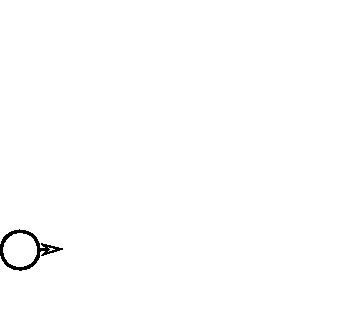
\includegraphics[width=0.44\textwidth]{slam_example_gt1.pdf}}
     }\hfill{}
     \subfloat[Robot SLAM system]
     {
     \fbox{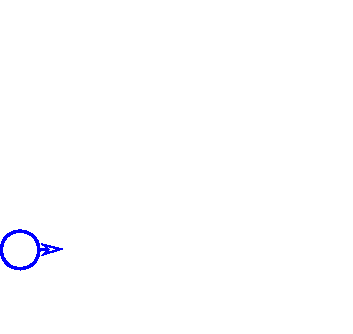
\includegraphics[width=0.44\textwidth]{slam_example_robot1.pdf}}
     }
     \end{figure}
    
    \end{frame}
    
    \begin{frame}
     \frametitle{SLAM example}

     \begin{figure}
     \subfloat[Reality]
     {
     \fbox{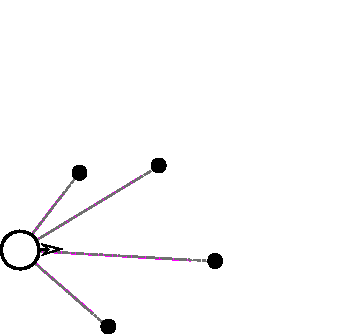
\includegraphics[width=0.44\textwidth]{slam_example_gt2.pdf}}
     }\hfill{}
     \subfloat[Robot SLAM system]
     {
     \fbox{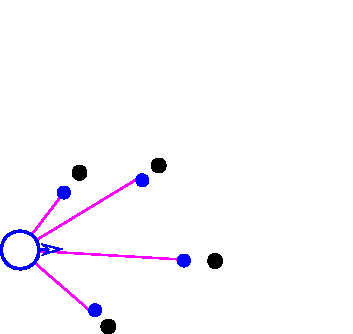
\includegraphics[width=0.44\textwidth]{slam_example_robot2.pdf}}
     }
     \end{figure}
    
    \end{frame}
    
    \begin{frame}
     \frametitle{SLAM example}
    
     \begin{figure}
     \subfloat[Reality]
     {
     \fbox{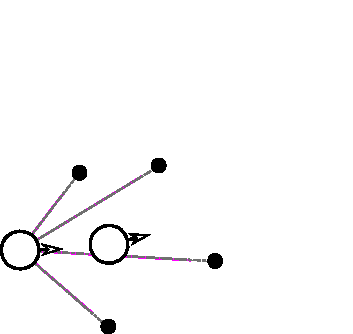
\includegraphics[width=0.44\textwidth]{slam_example_gt3.pdf}}
     }\hfill{}
     \subfloat[Robot SLAM system]
     {
     \fbox{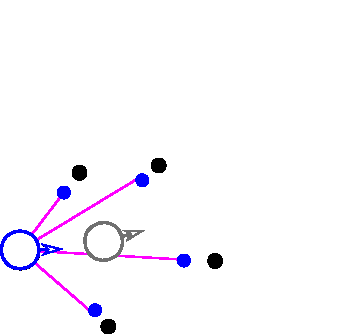
\includegraphics[width=0.44\textwidth]{slam_example_robot3.pdf}}
     }
     \end{figure}
    
    \end{frame}
    
    \begin{frame}
     \frametitle{SLAM example}
    
     \begin{figure}
     \subfloat[Reality]
     {
     \fbox{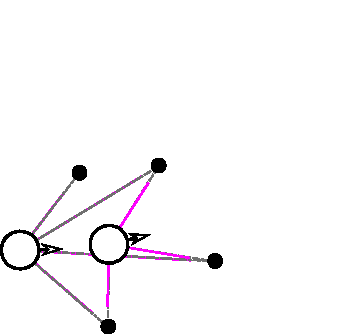
\includegraphics[width=0.44\textwidth]{slam_example_gt4.pdf}}
     }\hfill{}
     \subfloat[Robot SLAM system]
     {
     \fbox{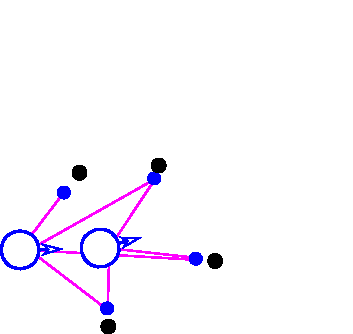
\includegraphics[width=0.44\textwidth]{slam_example_robot4.pdf}}
     }
     \end{figure}
    
    \end{frame}
    
    \begin{frame}
     \frametitle{SLAM example}
    
     \begin{figure}
     \subfloat[Reality]
     {
     \fbox{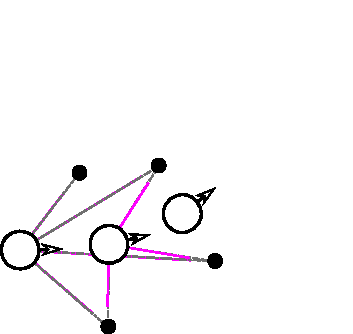
\includegraphics[width=0.44\textwidth]{slam_example_gt5.pdf}}
     }\hfill{}
     \subfloat[Robot SLAM system]
     {
     \fbox{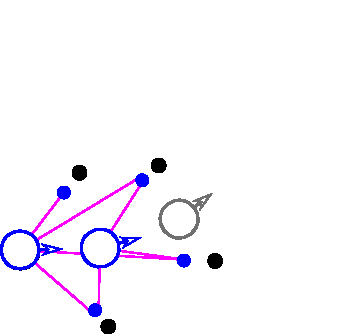
\includegraphics[width=0.44\textwidth]{slam_example_robot5.pdf}}
     }
     \end{figure}
    
    \end{frame}
    
    \begin{frame}
     \frametitle{SLAM example}
    
     \begin{figure}
     \subfloat[Reality]
     {
     \fbox{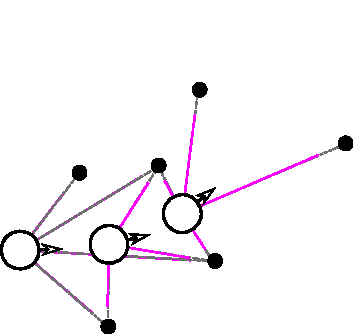
\includegraphics[width=0.44\textwidth]{slam_example_gt6.pdf}}
     }\hfill{}
     \subfloat[Robot SLAM system]
     {
     \fbox{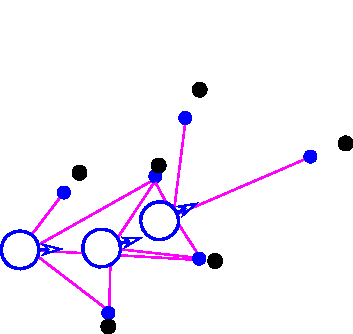
\includegraphics[width=0.44\textwidth]{slam_example_robot6.pdf}}
     }
     \end{figure}
    
    \end{frame}
    
    \begin{frame}
     \frametitle{SLAM example}
    
     \begin{figure}
     \subfloat[Reality]
     {
     \fbox{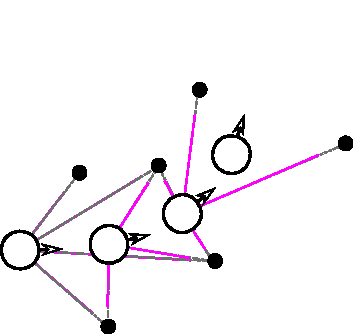
\includegraphics[width=0.44\textwidth]{slam_example_gt7.pdf}}
     }\hfill{}
     \subfloat[Robot SLAM system]
     {
     \fbox{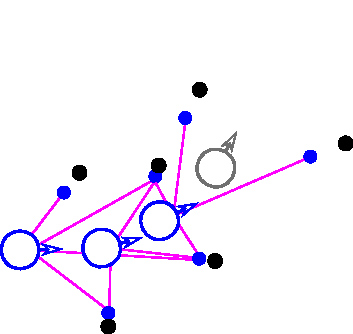
\includegraphics[width=0.44\textwidth]{slam_example_robot7.pdf}}
     }
     \end{figure}
    
    \end{frame}
    
    \begin{frame}
     \frametitle{SLAM example}
    
     \begin{figure}
     \subfloat[Reality]
     {
     \fbox{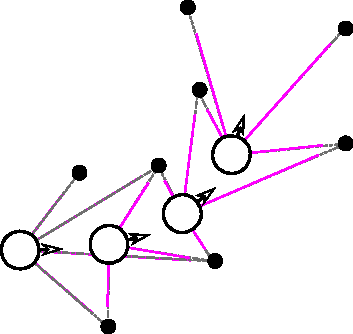
\includegraphics[width=0.44\textwidth]{slam_example_gt8.pdf}}
     }\hfill{}
     \subfloat[Robot SLAM system]
     {
     \fbox{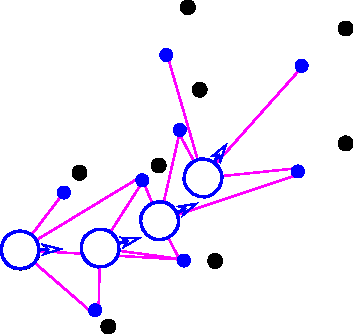
\includegraphics[width=0.44\textwidth]{slam_example_robot8.pdf}}
     }
     \end{figure}
    
    \end{frame}
    
    \begin{frame}
     \frametitle{General SLAM architecture}
    
     \begin{figure}[!h]
     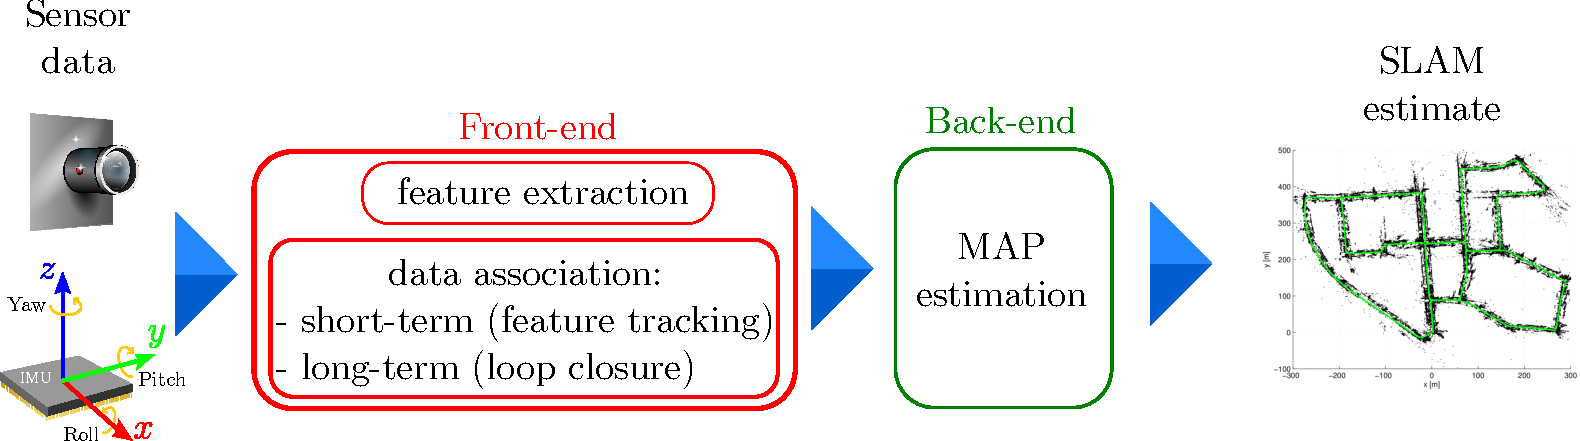
\includegraphics[width=\textwidth]{images/slam_frontend_backend.pdf}
     \end{figure}
    
\end{frame}

\begin{frame}
    \frametitle{Types of SLAM Back-ends}
    \note{Information taken from https://youtu.be/BuRCJ2fegcc and https://youtu.be/Alu59K8zvYs}
    \footnotesize
    \begin{itemize}
    \item Based on Kalman Filter (EKF-SLAM)
    \item Based on Particle Filter (FastSLAM, Rao-Blackwellized Particle Filter, Gmapping)
    \item Based on Least-Squares (Graph-SLAM, Bundle Adjustment)
    \begin{itemize}
    \item Pose-Graph (only contains the robot poses; the map is marginalized.\footnote{Marginalization is the process of removing variables without losing information.})
    \item Factor-Graph (contains poses and landmarks)
    \end{itemize}
    Optimization Tools
    \begin{itemize}
    \item Ceres
    \item GTSAM
    \item g2o
    \end{itemize}
    \end{itemize}
    
    \begin{center}
    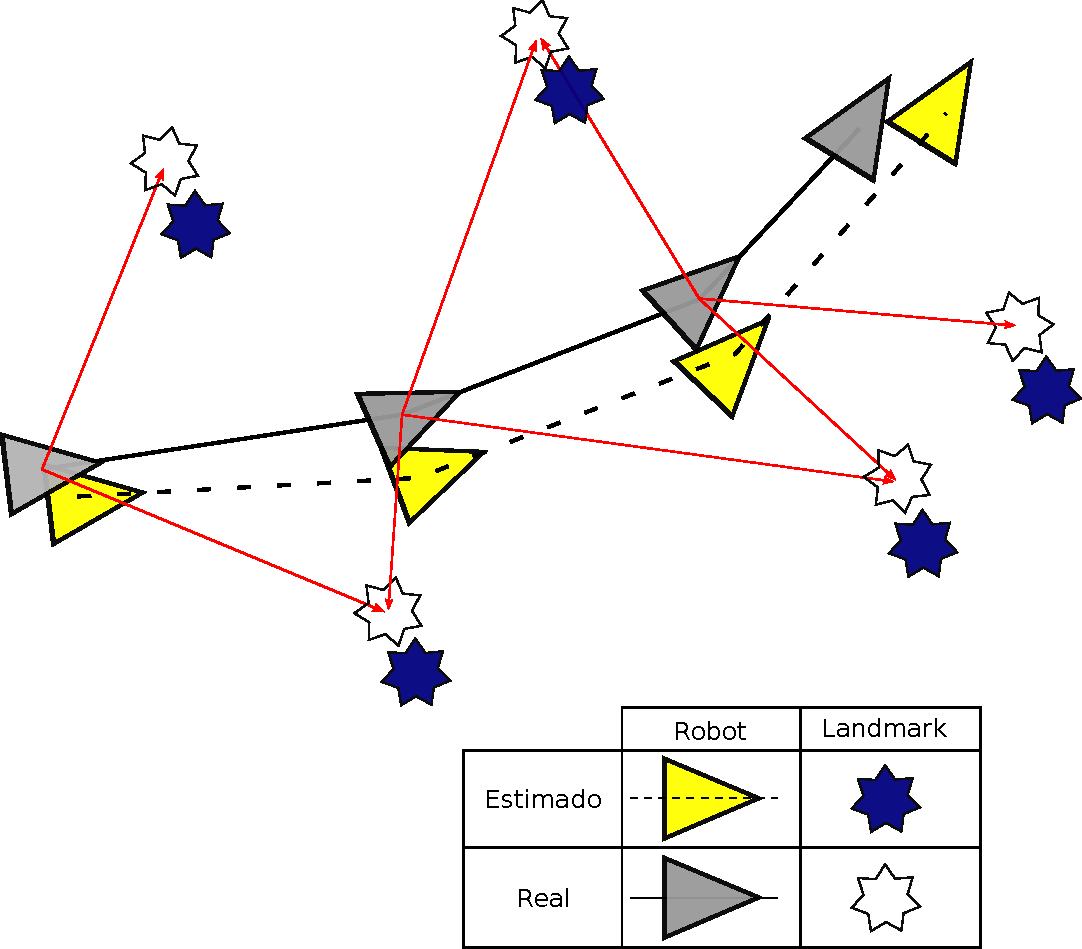
\includegraphics[width=0.25\textwidth]{images/slam-landmarks.pdf}
    \end{center}
    
    \end{frame}
    
    

	\section{EKF-SLAM}
	\begin{frame}
    \frametitle{SLAM Problem Definition}
    \note{Information taken from https://www.youtube.com/watch?v=X30sEgIws0g}
    \note{Information taken from https://www.ipb.uni-bonn.de/html/teaching/photo12-2021/2021-pho2-16-ekf-slam.pptx.pdf}
    
    Given:
    \begin{itemize}
        \item Control Commands Sent
    
            \begin{equation*}
            \controlCommand_{1:T} = \{\controlCommand_1, \controlCommand_2, \ldots, \controlCommand_T\}
            \end{equation*}
        \item Observations
            \begin{equation*}
            \observation_{1:T} = \{\observation_1, \observation_2, \ldots, \observation_T\} 
            \end{equation*} 
    \end{itemize} 
    
    Wanted: 
    \begin{itemize} 
        \item Environment map: $\map$ 
        \item Trajectory (or current pose) of the vehicle: 
        \begin{equation*} 
        \state_{0:T} = \{\state_0, \state_1, \ldots, \state_T\} \qquad \text{or} \qquad \state_{t} 
        \end{equation*} 
    \end{itemize}
\end{frame}
    
\begin{frame}
    \frametitle{Bayes Filter} 
    \note{Information taken from https://www.youtube.com/watch?v=X30sEgIws0g} 
    \note{Information extracted from https://www.ipb.uni-bonn.de/html/teaching/photo12-2021/2021-pho2-16-ekf-slam.pptx.pdf} 
    
    \begin{itemize} 
        \item Recursive filter with \textbf{prediction} and \textbf{correction} steps 
        \item Estimates: $p(x_t, \map | \observation _{1:t}, \controlCommand _{1:t})$ 
        \item Kalman Filter is a recursive Bayes Filter for the \textbf{linear Gaussian case} 
        \item \textbf{EKF} for dealing with \textbf{non-linearities} 
    \end{itemize}
\end{frame}

\begin{frame}
    \frametitle{Grafical Model of Full SLAM}
    \note{Información extraída de https://www.youtube.com/watch?v=X30sEgIws0g}
    \note{Información extraída de https://www.ipb.uni-bonn.de/html/teaching/photo12-2021/2021-pho2-16-ekf-slam.pptx.pdf}

    \[ p(\state_{1:t}, \map | \observation_{1:t}, \controlCommand_{1:t}) \]

    \begin{center}
        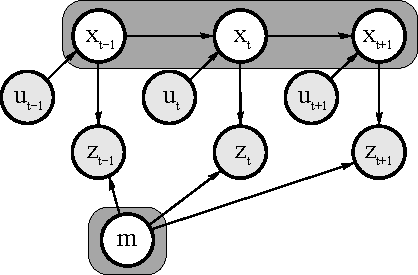
\includegraphics[width=0.6\textwidth]{../images/ekf_slam/graphical_model_full_slam.pdf}
    \end{center}
\end{frame}

\begin{frame}
    \frametitle{Grafical Model of Online SLAM}
    \note{Información extraída de https://www.youtube.com/watch?v=X30sEgIws0g}
    \note{Información extraída de https://www.ipb.uni-bonn.de/html/teaching/photo12-2021/2021-pho2-16-ekf-slam.pptx.pdf}

    We consider the Kalman filter as a solution to the online SLAM problem:
    \begin{equation*}
        p(\state_{t}, \map | \observation_{1:t}, \controlCommand_{1:t}) = \int \int \cdots \int p(\state_{1:t}, \map | \observation_{1:t}, \controlCommand_{1:t}) d\state_{1} d\state_{2} \ldots d\state_{t-1}
    \end{equation*}

    \begin{center}
        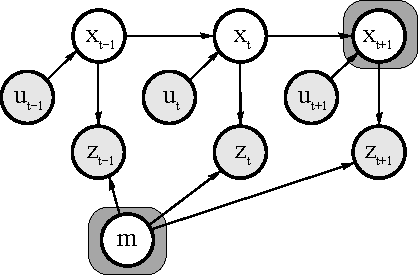
\includegraphics[width=0.6\textwidth]{../images/ekf_slam/graphical_model_online_slam.pdf}
    \end{center}

    \note{EKF can not adjust previous poses of the trajectory when a loop closure is done but can adjust the map and the current pose.}

\end{frame}

\begin{frame}
    \frametitle{Extended Kalman Filter Algorithm}
    \note{Información extraída de https://www.youtube.com/watch?v=X30sEgIws0g}
    \note{Información extraída de https://www.ipb.uni-bonn.de/html/teaching/photo12-2021/2021-pho2-16-ekf-slam.pptx.pdf}
    
    \begin{algorithmic}[1]
    \Procedure{ExtendedKalmanFilter}{$\mu_{t-1}, \covariance_{t-1}, \controlCommand_{t}, \observation_{t}$}
        \State $\overline{\mu}_{t} = \motionModelFunction{\controlCommand_{t}, \mu_{t-1}}$
        \State $\overline{\covariance}_{t} = \motionModelJacobian_{t} \covariance_{t-1} \motionModelJacobian_{t}^{\top}+\motionParametersCovariance_{t}$
        \Statex
        \State $\kalmanGain_{t} = \overline{\covariance}_{t} \observationModelJacobian_{t}^{\top} (\observationModelJacobian_{t} \overline{\covariance}_{t}  \observationModelJacobian_{t} + \observationModelCovariance_{t})^{-1} $
        \State $\mu_{t} = \overline{\mu}_{t} + \kalmanGain_{t} (\observation_{t} - \observationModelFunction{\overline{\mu}_{t}})$
        \State $\covariance_{t} =  (I - \kalmanGain_{t} \observationModelJacobian_{t}) \overline{\covariance}_{t}$
        \State \Return $\mu_{t}, \covariance_{t}$
    \EndProcedure
    \end{algorithmic}
\end{frame}

\begin{frame}
    \frametitle{EKF SLAM}
    \note{Información extraída de https://www.youtube.com/watch?v=X30sEgIws0g}
    \note{Información extraída de https://www.ipb.uni-bonn.de/html/teaching/photo12-2021/2021-pho2-16-ekf-slam.pptx.pdf}

    \begin{itemize}
        \item Application of EKF to SLAM
        \item Estimate robot's pose and landmark locations
        \item Assumption: known data association
        \item State space (for the 2D plane) is:
    \end{itemize}
    \[ x_t = (\underbrace{x, y, \theta}_{robot's pose}, \underbrace{\map_{1,x}, \map_{1,y}}_{\text{landmark 1}}, \ldots, \underbrace{\map_{n,x}, \map_{n,y}}_{\text{landmark n}} )^{\top} \]
\end{frame}

\begin{frame}
    \frametitle{EKF SLAM: State Representation}
    \note{Información extraída de https://www.youtube.com/watch?v=X30sEgIws0g}
    \note{Información extraída de https://www.ipb.uni-bonn.de/html/teaching/photo12-2021/2021-pho2-16-ekf-slam.pptx.pdf}

    \begin{itemize}
        \item Map with $n$ landmarks: $(3+2n)$-dimensional Gaussian
        \item Belief represented by:
        \begin{equation*}
            \underbrace{\begin{bNiceMatrix}[margin = 4pt]
                \CodeBefore
                \rectanglecolor{yellow!40}{1-1}{3-1}
                \rectanglecolor{blue!20}{4-1}{9-1}
                \Body
                x \\
                y \\
                \theta \\
                \map_{1,x} \\
                \map_{1,y} \\
                \vdots \\
                \map_{n,x} \\
                \map_{n,y}
            \end{bNiceMatrix}}_{\mu}
            \underbrace{\begin{bNiceMatrix}[margin = 4pt]
                \CodeBefore
                \rectanglecolor{yellow!40}{1-1}{3-3}
                \rectanglecolor{green!40}{1-4}{3-8}
                \rectanglecolor{green!40}{4-1}{8-3}
                \rectanglecolor{blue!20}{4-4}{8-8}
                \Body
                \sigma_{xx} & \sigma_{xy} & \sigma_{x\theta} & \sigma_{x \map_{1,x}} & \sigma_{x \map_{1,y}} & \cdots & \sigma_{x \map_{n,x}} & \sigma_{x \map_{n,y}}\\
                \sigma_{yx} & \sigma_{yy} & \sigma_{y\theta} & \sigma_{y \map_{1,x}} & \sigma_{y \map_{1,y}} & \cdots & \sigma_{y \map_{n,x}} & \sigma_{y \map_{n,y}}\\
                \sigma_{\theta x} & \sigma_{\theta y} & \sigma_{\theta\theta} & \sigma_{\theta \map_{1,x}} & \sigma_{\theta \map_{1,y}} & \cdots & \sigma_{\theta \map_{n,x}} & \sigma_{\theta \map_{n,y}}\\
                \sigma_{\map_{1,x}x} & \sigma_{\map_{1,x}y} & \sigma_{\map_{1,x}\theta} & \sigma_{\map_{1,x}\map_{1,x}} & \sigma_{\map_{1,x}\map_{1,y}} & \cdots & \sigma_{\map_{1,x} \map_{n,x}} & \sigma_{\map_{1,x} \map_{n,y}} \\
                \sigma_{\map_{1,y}x} & \sigma_{\map_{1,y}y} & \sigma_{\map_{1,y}\theta} & \sigma_{\map_{1,y}\map_{1,x}} & \sigma_{\map_{1,y}\map_{1,y}} & \cdots & \sigma_{\map_{1,y} \map_{n,x}} & \sigma_{\map_{1,y} \map_{n,y}} \\
                \vdots & \vdots & \vdots & \vdots & \vdots & \ddots & \vdots & \vdots \\
                \sigma_{\map_{n,x}x} & \sigma_{\map_{n,x}y} & \sigma_{\map_{n,x}\theta} & \sigma_{\map_{n,x} \map_{1,x}} & \sigma_{\map_{n,x} \map_{1,y}} &\cdots & \sigma_{\map_{n,x} \map_{n,x}} & \sigma_{\map_{n,x} \map_{n,y}} \\
                \sigma_{\map_{n,y}x} & \sigma_{\map_{n,y}y} & \sigma_{\map_{n,y}\theta} & \sigma_{\map_{n,y} \map_{1,x}} & \sigma_{\map_{n,y} \map_{1,y}} & \cdots & \sigma_{\map_{n,y} \map_{n,x}} & \sigma_{\map_{n,y} \map_{n,y}}
            \end{bNiceMatrix}}_{\Sigma}
        \end{equation*}
    \end{itemize}
\end{frame}

\begin{frame}
    \frametitle{EKF SLAM: State Representation}
    \note{Información extraída de https://www.youtube.com/watch?v=X30sEgIws0g}
    \note{Información extraída de https://www.ipb.uni-bonn.de/html/teaching/photo12-2021/2021-pho2-16-ekf-slam.pptx.pdf}

    \begin{itemize}
        \item Map with $n$ landmarks: $(3+2n)$-dimensional Gaussian
        \item Belief represented by:
        \begin{equation*}
            \underbrace{\begin{bNiceMatrix}[margin = 4pt]
                \CodeBefore
                \rectanglecolor{yellow!40}{1-1}{1-1}
                \rectanglecolor{blue!20}{2-1}{4-1}
                \Body
                \state_t \\
                \map_1 \\
                \vdots \\
                \map_n
            \end{bNiceMatrix}}_{\mu}
            \underbrace{\begin{bNiceMatrix}[margin = 4pt]
                \CodeBefore
                \rectanglecolor{yellow!40}{1-1}{1-1}
                \rectanglecolor{green!40}{2-1}{4-1}
                \rectanglecolor{green!40}{1-2}{1-4}
                \rectanglecolor{blue!20}{2-2}{4-4}
                \Body
                \Sigma_{\state_t \state_t} & \Sigma_{\state_t \map_1} & \cdots & \Sigma_{\state_t \map_n} \\
                \Sigma_{\map_1 \state_t} & \Sigma_{\map_1 \map_1} & \cdots & \Sigma_{\map_1 \map_n} \\
                \vdots & \vdots & \ddots & \vdots \\
                \Sigma_{\map_n \state_t} & \Sigma_{\map_n \map_1} & \cdots & \Sigma_{\map_n \map_n}
            \end{bNiceMatrix}}_{\Sigma}
        \end{equation*}
    \end{itemize}

    The matrix diagonal blocks (yellow and blue) are the covariance of the pose and landmarks. The green blocks links the landmarks with the pose.

\end{frame}

\begin{frame}
    \frametitle{EKF SLAM: State Representation}
    \note{Información extraída de https://www.youtube.com/watch?v=X30sEgIws0g}
    \note{Información extraída de https://www.ipb.uni-bonn.de/html/teaching/photo12-2021/2021-pho2-16-ekf-slam.pptx.pdf}

    \begin{itemize}
        \item More Compactly
        \begin{equation*}
            \underbrace{\begin{bNiceMatrix}[margin = 4pt]
                \CodeBefore
                \rectanglecolor{yellow!40}{1-1}{1-1}
                \rectanglecolor{blue!20}{2-1}{2-1}
                \Body
                \state\\
                \map
            \end{bNiceMatrix}}_{\mu}
            \underbrace{\begin{bNiceMatrix}[margin = 4pt]
                \CodeBefore
                \rectanglecolor{yellow!40}{1-1}{1-1}
                \rectanglecolor{green!40}{2-1}{2-1}
                \rectanglecolor{green!40}{1-2}{1-2}
                \rectanglecolor{blue!20}{2-2}{2-2}
                \Body
                \Sigma_{\state \state} & \Sigma_{\state \map} \\
                \Sigma_{\map \state} & \Sigma_{\map \map}
            \end{bNiceMatrix}}_{\Sigma}
        \end{equation*}
    \end{itemize}
\end{frame}

\begin{frame}
    \frametitle{EKF SLAM: Filter Cycle}
    \note{Información extraída de https://www.youtube.com/watch?v=X30sEgIws0g}
    \note{Información extraída de https://www.ipb.uni-bonn.de/html/teaching/photo12-2021/2021-pho2-16-ekf-slam.pptx.pdf}
    \begin{enumerate}
    \item State prediction
    \item Measurement prediction
    \item Measurement
    \item Data association
    \item Update
    \end{enumerate}
\end{frame}

\begin{frame}
    \frametitle{EKF SLAM: Initial State}
    \note{Información extraída de https://www.youtube.com/watch?v=X30sEgIws0g}
    \note{Información extraída de https://www.ipb.uni-bonn.de/html/teaching/photo12-2021/2021-pho2-16-ekf-slam.pptx.pdf}


    \begin{center}
        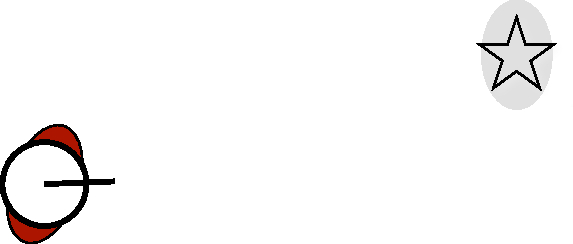
\includegraphics[width=0.4\textwidth]{./ekf_slam/ekf_slam_initial_state.pdf}
    \end{center}

    \begin{equation*}
        \underbrace{\begin{bNiceMatrix}
            \state_t \\
            \map_1 \\
            \vdots \\
            \map_n
        \end{bNiceMatrix}}_{\mu}
        \underbrace{\begin{bNiceMatrix}
            \Sigma_{\state_t \state_t} & \Sigma_{\state_t \map_1} & \cdots & \Sigma_{\state_t \map_n} \\
            \Sigma_{\map_1 \state_t} & \Sigma_{\map_1 \map_1} & \cdots & \Sigma_{\map_1 \map_n} \\
            \vdots & \vdots & \ddots & \vdots \\
            \Sigma_{\map_n \state_t} & \Sigma_{\map_n \map_1} & \cdots & \Sigma_{\map_n \map_n}
        \end{bNiceMatrix}}_{\Sigma}
    \end{equation*}
\end{frame}

\begin{frame}
    \frametitle{EKF SLAM: Predicted Motion}
    \note{Información extraída de https://www.youtube.com/watch?v=X30sEgIws0g}
    \note{Información extraída de https://www.ipb.uni-bonn.de/html/teaching/photo12-2021/2021-pho2-16-ekf-slam.pptx.pdf}


    \begin{center}
        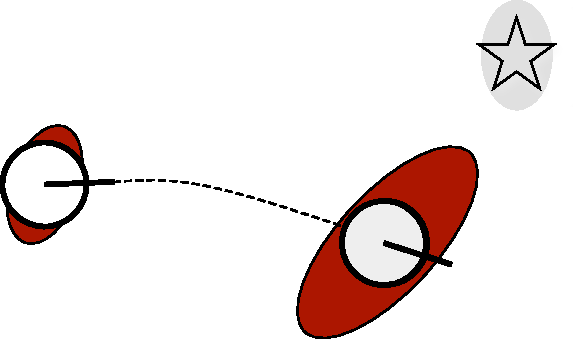
\includegraphics[width=0.4\textwidth]{../images/ekf_slam/ekf_slam_predicted_motion.pdf}
    \end{center}

    \begin{equation*}
        \underbrace{\begin{bNiceMatrix}[margin = 4pt]
            \CodeBefore
            \rectanglecolor{green!40}{1-1}{1-1}
            \Body
            \state_t \\
            \map_1 \\
            \vdots \\
            \map_n
        \end{bNiceMatrix}}_{\mu}
        \underbrace{\begin{bNiceMatrix}[margin = 4pt]
            \CodeBefore
            \rectanglecolor{green!40}{1-1}{1-4}
            \rectanglecolor{green!40}{1-1}{4-1}
            \Body
            \Sigma_{\state_t \state_t} & \Sigma_{\state_t \map_1} & \cdots & \Sigma_{\state_t \map_n} \\
            \Sigma_{\map_1 \state_t} & \Sigma_{\map_1 \map_1} & \cdots & \Sigma_{\map_1 \map_n} \\
            \vdots & \vdots & \ddots & \vdots \\
            \Sigma_{\map_n \state_t} & \Sigma_{\map_n \map_1} & \cdots & \Sigma_{\map_n \map_n}
        \end{bNiceMatrix}}_{\Sigma}
    \end{equation*}

    \tiny

    If the robot moves, the uncertainty increases and we must update the robot pose and the correlation between the robot and the landmarks. The latter happens because now the pose provides less information about the landmarks since the robot got more uncertainty about its pose. The landmarks are not updated since the robot motion does not affect the position of the landmarks.

\end{frame}

\begin{frame}
    \frametitle{EKF SLAM: Predicted Measurement}
    \note{Información extraída de https://www.youtube.com/watch?v=X30sEgIws0g}
    \note{Información extraída de https://www.ipb.uni-bonn.de/html/teaching/photo12-2021/2021-pho2-16-ekf-slam.pptx.pdf}

    Given the predicted pose and the landmark location, we predict the measurement we should obtain.

    \begin{center}
        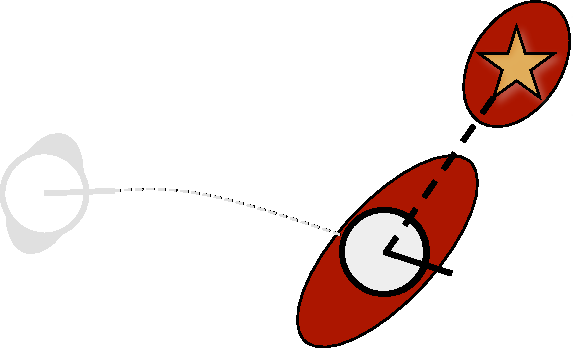
\includegraphics[width=0.4\textwidth]{../images/ekf_slam/ekf_slam_predicted_measurement.pdf}
    \end{center}

    \begin{equation*}
        \underbrace{\begin{bNiceMatrix}
            \state_t \\
            \map_1 \\
            \vdots \\
            \map_n
        \end{bNiceMatrix}}_{\mu}
        \underbrace{\begin{bNiceMatrix}
            \Sigma_{\state_t \state_t} & \Sigma_{\state_t \map_1} & \cdots & \Sigma_{\state_t \map_n} \\
            \Sigma_{\map_1 \state_t} & \Sigma_{\map_1 \map_1} & \cdots & \Sigma_{\map_1 \map_n} \\
            \vdots & \vdots & \ddots & \vdots \\
            \Sigma_{\map_n \state_t} & \Sigma_{\map_n \map_1} & \cdots & \Sigma_{\map_n \map_n}
        \end{bNiceMatrix}}_{\Sigma}
    \end{equation*}
\end{frame}

\begin{frame}
    \frametitle{EKF SLAM: Obtained Measurement}
    \note{Información extraída de https://www.youtube.com/watch?v=X30sEgIws0g}
    \note{Información extraída de https://www.ipb.uni-bonn.de/html/teaching/photo12-2021/2021-pho2-16-ekf-slam.pptx.pdf}

    The sensor observes the landmark.

    \begin{center}
        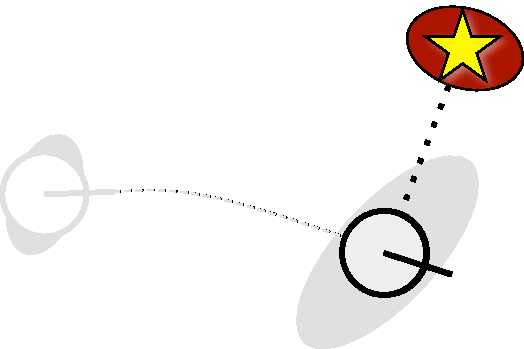
\includegraphics[width=0.4\textwidth]{../images/ekf_slam/ekf_slam_obtained_measurement.pdf}
    \end{center}

    \begin{equation*}
        \underbrace{\begin{bNiceMatrix}
            \state_t \\
            \map_1 \\
            \vdots \\
            \map_n
        \end{bNiceMatrix}}_{\mu}
        \underbrace{\begin{bNiceMatrix}
            \Sigma_{\state_t \state_t} & \Sigma_{\state_t \map_1} & \cdots & \Sigma_{\state_t \map_n} \\
            \Sigma_{\map_1 \state_t} & \Sigma_{\map_1 \map_1} & \cdots & \Sigma_{\map_1 \map_n} \\
            \vdots & \vdots & \ddots & \vdots \\
            \Sigma_{\map_n \state_t} & \Sigma_{\map_n \map_1} & \cdots & \Sigma_{\map_n \map_n}
        \end{bNiceMatrix}}_{\Sigma}
    \end{equation*}
\end{frame}

\begin{frame}
    \frametitle{EKF SLAM: Data Association and Difference Between $h(x)$ and $\observation$}
    \note{Información extraída de https://www.youtube.com/watch?v=X30sEgIws0g}
    \note{Información extraída de https://www.ipb.uni-bonn.de/html/teaching/photo12-2021/2021-pho2-16-ekf-slam.pptx.pdf}

    \begin{center}
        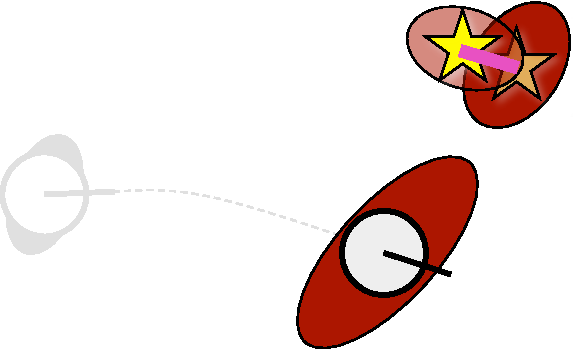
\includegraphics[width=0.4\textwidth]{../images/ekf_slam/ekf_slam_difference_between_prediction_observation.pdf}
    \end{center}

    \begin{equation*}
        \underbrace{\begin{bNiceMatrix}
            \state_t \\
            \map_1 \\
            \vdots \\
            \map_n
        \end{bNiceMatrix}}_{\mu}
        \underbrace{\begin{bNiceMatrix}
            \Sigma_{\state_t \state_t} & \Sigma_{\state_t \map_1} & \cdots & \Sigma_{\state_t \map_n} \\
            \Sigma_{\map_1 \state_t} & \Sigma_{\map_1 \map_1} & \cdots & \Sigma_{\map_1 \map_n} \\
            \vdots & \vdots & \ddots & \vdots \\
            \Sigma_{\map_n \state_t} & \Sigma_{\map_n \map_1} & \cdots & \Sigma_{\map_n \map_n}
        \end{bNiceMatrix}}_{\Sigma}
    \end{equation*}
\end{frame}

\begin{frame}
    \frametitle{EKF SLAM: Update Step}
    \note{Información extraída de https://www.youtube.com/watch?v=X30sEgIws0g}
    \note{Información extraída de https://www.ipb.uni-bonn.de/html/teaching/photo12-2021/2021-pho2-16-ekf-slam.pptx.pdf}


    \begin{center}
        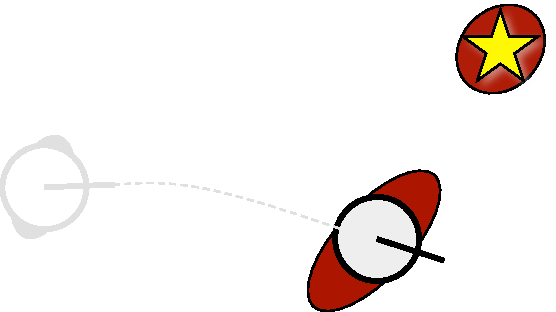
\includegraphics[width=0.4\textwidth]{../images/ekf_slam/ekf_slam_update.pdf}
    \end{center}

    \begin{equation*}
        \underbrace{\begin{bNiceMatrix}[margin = 4pt]
            \CodeBefore
            \rectanglecolor{green!40}{1-1}{4-1}
            \Body
            \state_t \\
            \map_1 \\
            \vdots \\
            \map_n
        \end{bNiceMatrix}}_{\mu}
        \underbrace{\begin{bNiceMatrix}[margin = 4pt]
            \CodeBefore
            \rectanglecolor{green!40}{1-1}{4-4}
            \Body
            \Sigma_{\state_t \state_t} & \Sigma_{\state_t \map_1} & \cdots & \Sigma_{\state_t \map_n} \\
            \Sigma_{\map_1 \state_t} & \Sigma_{\map_1 \map_1} & \cdots & \Sigma_{\map_1 \map_n} \\
            \vdots & \vdots & \ddots & \vdots \\
            \Sigma_{\map_n \state_t} & \Sigma_{\map_n \map_1} & \cdots & \Sigma_{\map_n \map_n}
        \end{bNiceMatrix}}_{\Sigma}
    \end{equation*}

    The robot pose and the landmarks locations are corrected along the whole covariance matrix.
\end{frame}

\begin{frame}
    \frametitle{EKF SLAM: Concrete Example}
    \note{Información extraída de https://www.youtube.com/watch?v=X30sEgIws0g}
    \note{Información extraída de https://www.ipb.uni-bonn.de/html/teaching/photo12-2021/2021-pho2-16-ekf-slam.pptx.pdf}

    Setup:
    \begin{itemize}
        \item Platform moves in the 2D plane
        \item Velocity-based motion model
        \item Observation of point landmarks (e.g. corners or columns)
        \item Range-bearing sensor (measures distance and angle to landmarks)
        \item Known data association (which measurement comes from which landmark)
        \item Known number of landmarks (This is not a constraint but its implementation need some checks in the algorithm: check if the state vector is full requiring to do some bookkeeping). \note{We leave it out of this lecture because It will drag away the attention to the important concepts.}
    \end{itemize}
\end{frame}

\begin{frame}
    \frametitle{Initialization}
    \note{Información extraída de https://www.youtube.com/watch?v=X30sEgIws0g}
    \note{Información extraída de https://www.ipb.uni-bonn.de/html/teaching/photo12-2021/2021-pho2-16-ekf-slam.pptx.pdf}

    \begin{itemize}
        \item Platform starts in its own reference frame
        \item All landmarks are initially unknown (not yet observed)
        \item State vector dimension: $2N + 3$ \\
        (3 for robot pose + $2N$ for $N$ landmarks in 2D space)
        \begin{equation*}
            \mu_0 =
            \begin{bmatrix}
                0 & 0 & 0 & \dots & 0    
            \end{bmatrix}^{\top}
        \end{equation*}
    \end{itemize}
    
    \begin{equation*}
        \Sigma_0 =
        \begin{bmatrix}
            \Sigma_{x_0} & 0 & \cdots & 0 \\
            0 & \infty I_{2} & \cdots & 0 \\
            \vdots & \vdots & \ddots & \vdots \\
            0 & 0 & \cdots & \infty I_{2}
        \end{bmatrix}
    \end{equation*}
    
    \begin{itemize}
        \item $\Sigma_{x_0}$: Initial uncertainty in robot pose (typically  a zero matrix or small)
        \item $\infty I_{2}$: Infinite uncertainty for unobserved landmarks (In practice we don't use infinite to avoid numerical issues)
    \end{itemize}

    \note{We can limit the use of landmark by their index. Each time the landmark a new landmark is observed we increase the index so that landmark is incorporated to the state and the covariance matrix. We do this until we reach the maximum of landmarks that we can work with.}

\end{frame}

\begin{frame}
    \frametitle{Extended Kalman Filter Algorithm}
    \note{Información extraída de https://www.youtube.com/watch?v=X30sEgIws0g}
    \note{Información extraída de https://www.ipb.uni-bonn.de/html/teaching/photo12-2021/2021-pho2-16-ekf-slam.pptx.pdf}
    
    \begin{algorithmic}[1]
    \Procedure{ExtendedKalmanFilter}{$\mu_{t-1}, \covariance_{t-1}, \controlCommand_{t}, \observation_{t}$}
        \State $\overline{\mu}_{t} = \alert{\motionModelFunction{\controlCommand_{t}, \mu_{t-1}}}$
        \State $\overline{\covariance}_{t} = \motionModelJacobian_{t} \covariance_{t-1} \motionModelJacobian_{t}^{\top}+\motionParametersCovariance_{t}$
        \Statex
        \State $\kalmanGain_{t} = \overline{\covariance}_{t} \observationModelJacobian_{t}^{\top} (\observationModelJacobian_{t} \overline{\covariance}_{t}  \observationModelJacobian_{t} + \observationModelCovariance_{t})^{-1} $
        \State $\mu_{t} = \overline{\mu}_{t} + \kalmanGain_{t} (\observation_{t} - \observationModelFunction{\overline{\mu}_{t}})$
        \State $\covariance_{t} =  (I - \kalmanGain_{t} \observationModelJacobian_{t}) \overline{\covariance}_{t}$
        \State \Return $\mu_{t}, \covariance_{t}$
    \EndProcedure
    \end{algorithmic}
\end{frame}

\begin{frame}
    \frametitle{Prediction Step (Motion)}
    \note{Información extraída de https://www.youtube.com/watch?v=X30sEgIws0g}
    \note{Información extraída de https://www.ipb.uni-bonn.de/html/teaching/photo12-2021/2021-pho2-16-ekf-slam.pptx.pdf}

    \begin{itemize}
        \item Goa: Update the state space based on the motion
        \item Motion in the plane (with a differential drive robot):
        \begin{equation*}
            \begin{bmatrix} x' \\ y' \\ \theta' \end{bmatrix} = 
            \underbrace{\begin{bmatrix} x \\ y \\ \theta \end{bmatrix} + 
            \begin{bmatrix} 
            -\frac{v_t}{\omega_t} \sin \theta + \frac{v_t}{\omega_t} \sin (\theta + \omega_t \Delta t) \\ 
            \frac{v_t}{\omega_t} \cos \theta - \frac{v_t}{\omega_t} \cos (\theta + \omega_t \Delta t) \\ 
            \omega_t \Delta t 
            \end{bmatrix}}_{g_{x,y,\theta}\left(\controlCommand_{t}, \begin{bmatrix} x & y & \theta \end{bmatrix}^{\top}\right)}
        \end{equation*}
        \item How to map that to the $2N+3$ dimmension state space used in EKF?
    \end{itemize}

\end{frame}

\begin{frame}
    \frametitle{Update the State Space}
    \note{Información extraída de https://www.youtube.com/watch?v=X30sEgIws0g}
    \note{Información extraída de https://www.ipb.uni-bonn.de/html/teaching/photo12-2021/2021-pho2-16-ekf-slam.pptx.pdf}

    \begin{itemize}
        \item From the motion in the plane
        
        \begin{equation*}
            \begin{bmatrix} x' \\ y' \\ \theta' \end{bmatrix} = 
            \underbrace{\begin{bmatrix} x \\ y \\ \theta \end{bmatrix} + 
            \begin{bmatrix} 
            -\frac{v_t}{\omega_t} \sin \theta + \frac{v_t}{\omega_t} \sin (\theta + \omega_t \Delta t) \\ 
            \frac{v_t}{\omega_t} \cos \theta - \frac{v_t}{\omega_t} \cos (\theta + \omega_t \Delta t) \\ 
            \omega_t \Delta t 
            \end{bmatrix}}_{g_{x,y,\theta}\left(\controlCommand_{t}, \begin{bmatrix} x, y, \theta \end{bmatrix}^{\top}\right)}
        \end{equation*}
    

        \item To the \(2N+3\) dimensional space:
        \begin{equation*}
            \begin{bmatrix}
            x' \\
            y' \\
            \theta'\\
            \vdots
            \end{bmatrix}
            =
            \underbrace{\begin{bmatrix}
            x \\
            y \\
            \theta\\
            \vdots
            \end{bmatrix}
            +
            \underbrace{\begin{bNiceMatrix}[margin = 3 pt]
            1 & 0 & 0 & 0 & \ldots & 0 \\
            0 & 1 & 0 & 0 & \ldots & 0 \\
            0 & 0 & 1 & 0 & \ldots & 0 \\
            & & & & &
            \CodeAfter
            \UnderBrace{3-4}{3-6}{2N cols}
            \end{bNiceMatrix}^{\top}}_{F_{x}^{\top}}
            \begin{bmatrix}
            -\frac{v_t}{\omega_t} \sin \theta + \frac{v_t}{\omega_t} \sin (\theta + \omega_t \Delta t) \\
            \frac{v_t}{\omega_t} \cos \theta - \frac{v_t}{\omega_t} \cos (\theta + \omega_t \Delta t) \\
            \omega_t \Delta t
            \end{bmatrix}}_{g(\controlCommand_{t}, \state_t)}
        \end{equation*}
    \end{itemize}

    \note{F is the mapping function that allows to update the state only in the pose components using the motion model.}
\end{frame}

\begin{frame}
    \frametitle{Extended Kalman Filter Algorithm}
    \note{Información extraída de https://www.youtube.com/watch?v=X30sEgIws0g}
    \note{Información extraída de https://www.ipb.uni-bonn.de/html/teaching/photo12-2021/2021-pho2-16-ekf-slam.pptx.pdf}
    
    \begin{algorithmic}[1]
    \Procedure{ExtendedKalmanFilter}{$\mu_{t-1}, \covariance_{t-1}, \controlCommand_{t}, \observation_{t}$}
        \State $\overline{\mu}_{t} = \motionModelFunction{\controlCommand_{t}, \mu_{t-1}}$
        \State $\alert{\overline{\covariance}_{t} = \motionModelJacobian_{t} \covariance_{t-1} \motionModelJacobian_{t}^{\top}+\motionParametersCovariance_{t}}$
        \Statex
        \State $\kalmanGain_{t} = \overline{\covariance}_{t} \observationModelJacobian_{t}^{\top} (\observationModelJacobian_{t} \overline{\covariance}_{t}  \observationModelJacobian_{t} + \observationModelCovariance_{t})^{-1} $
        \State $\mu_{t} = \overline{\mu}_{t} + \kalmanGain_{t} (\observation_{t} - \observationModelFunction{\overline{\mu}_{t}})$
        \State $\covariance_{t} =  (I - \kalmanGain_{t} \observationModelJacobian_{t}) \overline{\covariance}_{t}$
        \State \Return $\mu_{t}, \covariance_{t}$
    \EndProcedure
    \end{algorithmic}
\end{frame}

\begin{frame}
    \frametitle{Update Covariance}
    \note{Información extraída de https://www.youtube.com/watch?v=X30sEgIws0g}
    \note{Información extraída de https://www.ipb.uni-bonn.de/html/teaching/photo12-2021/2021-pho2-16-ekf-slam.pptx.pdf}

    \begin{itemize}
        \item The function $g$ only affects de motion and not the landmarks
    \end{itemize}

    Jacobian:
    \begin{equation*}
        G_t = 
        \begin{bmatrix}
            G_{t}^{\state} & 0 \\
            0 & I
        \end{bmatrix}
    \end{equation*}
    where $G_{t}^{\state}$ is the $3 \times 3$ Jacobian of the motion and $I$ is the $2N \times 2N$ identity matrix.


    Note that the Identity submatrix $I$ means that landmarks covariances would not change (it would remains the same as the previous covariance).

\end{frame}

\begin{frame}
    \frametitle{Jacobian of the Motion}
    \note{Información extraída de https://www.youtube.com/watch?v=X30sEgIws0g}
    \note{Información extraída de https://www.ipb.uni-bonn.de/html/teaching/photo12-2021/2021-pho2-16-ekf-slam.pptx.pdf}
    
    The Jacobian matrix $G_{t}^{\state}$ for the motion model is computed as:
    
    \begin{align*}
        G_{t}^{\state} &= \frac{\partial}{\partial(x, y, \theta)^{\top}} \left(
        \begin{bmatrix}
        x \\
        y \\
        \theta
        \end{bmatrix}
        +
        \begin{bmatrix}
        -\frac{v_t}{\omega_t} \sin \theta + \frac{v_t}{\omega_t} \sin(\theta + \omega_t \Delta t) \\
        \frac{v_t}{\omega_t} \cos \theta - \frac{v_t}{\omega_t} \cos(\theta + \omega_t \Delta t) \\
        \omega_t \Delta t
        \end{bmatrix}
        \right) \\
        &= I + \frac{\partial}{\partial(x, y, \theta)^{\top}} 
        \begin{bmatrix}
        -\frac{v_t}{\omega_t} \sin \theta + \frac{v_t}{\omega_t} \sin(\theta + \omega_t \Delta t) \\
        \frac{v_t}{\omega_t} \cos \theta - \frac{v_t}{\omega_t} \cos(\theta + \omega_t \Delta t) \\
        \omega_t \Delta t
        \end{bmatrix} \\
        &= I + 
        \begin{bmatrix}
        0 & 0 & -\frac{v_t}{\omega_t} \cos \theta + \frac{v_t}{\omega_t} \cos(\theta + \omega_t \Delta t) \\
        0 & 0 & -\frac{v_t}{\omega_t} \sin \theta + \frac{v_t}{\omega_t} \sin(\theta + \omega_t \Delta t) \\
        0 & 0 & 0
        \end{bmatrix} \\
        &= 
        \begin{bmatrix}
        1 & 0 & -\frac{v_t}{\omega_t} \cos \theta + \frac{v_t}{\omega_t} \cos(\theta + \omega_t \Delta t) \\
        0 & 1 & -\frac{v_t}{\omega_t} \sin \theta + \frac{v_t}{\omega_t} \sin(\theta + \omega_t \Delta t) \\
        0 & 0 & 1
        \end{bmatrix}
    \end{align*}
    
\end{frame}

\begin{frame}
    \frametitle{This leads to the Covariance update}
    \note{Información extraída de https://www.youtube.com/watch?v=X30sEgIws0g}
    \note{Información extraída de https://www.ipb.uni-bonn.de/html/teaching/photo12-2021/2021-pho2-16-ekf-slam.pptx.pdf}

    \begin{align*}
        \bar{\Sigma}_t &= G_t \Sigma_{t-1} G_t^{\top} + R_t \\
        &= 
        \begin{bmatrix}
        G_{t}^{\state} & 0 \\
        0 & I
        \end{bmatrix}
        \begin{bmatrix}
        \Sigma_{xx} & \Sigma_{xm} \\
        \Sigma_{mx} & \Sigma_{mm}
        \end{bmatrix}
        \begin{bmatrix}
        (G_{t}^{\state})^{\top} & 0 \\
        0 & I
        \end{bmatrix}
        + R_t \\
        &=
        \begin{bmatrix}
        G_{t}^{\state} \Sigma_{xx} (G_{t}^{\state})^{\top} & G_{t}^{\state} \Sigma_{xm} \\
        (G_{t}^{\state} \Sigma_{xm})^{\top} & \Sigma_{mm}
        \end{bmatrix}
        + R_t
    \end{align*}

\end{frame}

\begin{frame}
    \frametitle{EKF SLAM: Prediction Step}
    \note{Información extraída de https://www.youtube.com/watch?v=X30sEgIws0g}
    \note{Información extraída de https://www.ipb.uni-bonn.de/html/teaching/photo12-2021/2021-pho2-16-ekf-slam.pptx.pdf}

    \begin{algorithmic}[1]
        \Procedure{EKF\_SLAM\_Prediction}{$\mu_{t-1}, \Sigma_{t-1}, \controlCommand_t, \observation_t, c_t, R_t$}
        \State $F_{\state} = \begin{bmatrix}
        1 & 0 & 0 & 0 & 0 & \cdots & 0 \\
        0 & 1 & 0 & 0 & 0 & \cdots & 0 \\
        0 & 0 & 1 & 0 & 0 & \cdots & 0 \\
        \end{bmatrix}$
        \vspace{1em}
        \State $\bar{\mu}_t = \mu_{t-1} + F_x^{\top}
        \begin{bmatrix}
        \frac{-v_t}{\omega_t} \sin(\mu_{t-1,\theta}) + \frac{v_t}{\omega_t} \sin(\mu_{t-1,\theta} + \omega_t \Delta t) \\
        \frac{v_t}{\omega_t} \cos(\mu_{t-1,\theta}) - \frac{v_t}{\omega_t} \cos(\mu_{t-1,\theta} + \omega_t \Delta t) \\
        \omega_t \Delta t
        \end{bmatrix}$
        \vspace{1em}
        \State $G_t = I + F_{\state}^{\top}
        \begin{bmatrix}
        0 & 0 & \frac{-v_t}{\omega_t} \cos(\mu_{t-1,\theta}) + \frac{v_t}{\omega_t} \cos(\mu_{t-1,\theta} + \omega_t \Delta t) \\
        0 & 0 & \frac{-v_t}{\omega_t} \sin(\mu_{t-1,\theta}) + \frac{v_t}{\omega_t} \sin(\mu_{t-1,\theta} + \omega_t \Delta t) \\
        0 & 0 & 0
        \end{bmatrix} F_{\state}$
        \vspace{1em}
        \State $\bar{\Sigma}_t = G_{t} \Sigma_{t-1} G_{t}^{\top} + \underbrace{F_{\state}^{\top} R_{t}^{\state} F_{\state}}_{R_t}$
        \EndProcedure
    \end{algorithmic}
    
\end{frame}

\begin{frame}
    \frametitle{Extended Kalman Filter Algorithm}
    \note{Información extraída de https://www.youtube.com/watch?v=X30sEgIws0g}
    \note{Información extraída de https://www.ipb.uni-bonn.de/html/teaching/photo12-2021/2021-pho2-16-ekf-slam.pptx.pdf}
    
    \begin{algorithmic}[1]
    \Procedure{ExtendedKalmanFilter}{$\mu_{t-1}, \covariance_{t-1}, \controlCommand_{t}, \observation_{t}$}
        \State $\overline{\mu}_{t} = \motionModelFunction{\controlCommand_{t}, \mu_{t-1}}$
        \State $\overline{\covariance}_{t} = \motionModelJacobian_{t} \covariance_{t-1} \motionModelJacobian_{t}^{\top}+\motionParametersCovariance_{t}$
        \Statex
        \State $\alert{\kalmanGain_{t} = \overline{\covariance}_{t} \observationModelJacobian_{t}^{\top} (\observationModelJacobian_{t} \overline{\covariance}_{t}  \observationModelJacobian_{t} + \observationModelCovariance_{t})^{-1}}$
        \State $\alert{\mu_{t} = \overline{\mu}_{t} + \kalmanGain_{t} (\observation_{t} - \observationModelFunction{\overline{\mu}_{t}})}$
        \State $\alert{\covariance_{t} =  (I - \kalmanGain_{t} \observationModelJacobian_{t}) \overline{\covariance}_{t}}$
        \State \Return $\mu_{t}, \covariance_{t}$
    \EndProcedure
    \end{algorithmic}
\end{frame}

\begin{frame}
    \frametitle{EKF SLAM: Correction Step}
    \note{Información extraída de https://www.youtube.com/watch?v=X30sEgIws0g}
    \note{Información extraída de https://www.ipb.uni-bonn.de/html/teaching/photo12-2021/2021-pho2-16-ekf-slam.pptx.pdf}

    \begin{itemize}
        \item Known data association
        \item $c_{t}^{i} = j$ : $i$-th measurement at time $t$ observes the landmark with index $j$
        \item Initialize landmark if unobserved
        \item Compute the expected observation
        \item Compute the Jacobian of $h$
        \item Proceed with computing the Kalman gain
    \end{itemize}

\end{frame}

\begin{frame}
    \frametitle{Extended Kalman Filter Algorithm}
    \note{Información extraída de https://www.youtube.com/watch?v=X30sEgIws0g}
    \note{Información extraída de https://www.ipb.uni-bonn.de/html/teaching/photo12-2021/2021-pho2-16-ekf-slam.pptx.pdf}
    
    \begin{algorithmic}[1]
    \Procedure{ExtendedKalmanFilter}{$\mu_{t-1}, \covariance_{t-1}, \controlCommand_{t}, \observation_{t}$}
        \State $\overline{\mu}_{t} = \motionModelFunction{\controlCommand_{t}, \mu_{t-1}}$
        \State $\overline{\covariance}_{t} = \motionModelJacobian_{t} \covariance_{t-1} \motionModelJacobian_{t}^{\top}+\motionParametersCovariance_{t}$
        \Statex
        \State $\kalmanGain_{t} = \overline{\covariance}_{t} \alert{\observationModelJacobian_{t}^{\top}} (\observationModelJacobian_{t} \overline{\covariance}_{t}  \observationModelJacobian_{t} + \observationModelCovariance_{t})^{-1} $
        \State $\mu_{t} = \overline{\mu}_{t} + \kalmanGain_{t} (\observation_{t} - \observationModelFunction{\overline{\mu}_{t}})$
        \State $\covariance_{t} =  (I - \kalmanGain_{t} \observationModelJacobian_{t}) \overline{\covariance}_{t}$
        \State \Return $\mu_{t}, \covariance_{t}$
    \EndProcedure
    \end{algorithmic}
\end{frame}

\begin{frame}
    \frametitle{Range-Bearing Observation}
    \note{Información extraída de https://www.youtube.com/watch?v=X30sEgIws0g}
    \note{Información extraída de https://www.ipb.uni-bonn.de/html/teaching/photo12-2021/2021-pho2-16-ekf-slam.pptx.pdf}

    \begin{itemize}
        \item Range-Bearing observation $\observation_t^i = \begin{bmatrix} r_t^i \\ \phi_t^i \end{bmatrix}^{\top}$
        
        \item If landmark has not been observed, we can initialize it with:
    \end{itemize}
    
    \begin{equation*}
        \underbrace{
        \begin{bmatrix}
        \bar{\mu}_{j,x} \\
        \bar{\mu}_{j,y}
        \end{bmatrix}}_{\parbox{2cm}{\centering \scriptsize \text{location of} \\ \text{landmark} j}}
        =
        \underbrace{
        \begin{bmatrix}
        \bar{\mu}_{t,x} \\
        \bar{\mu}_{t,y}
        \end{bmatrix}}_{\parbox{2cm}{\centering \scriptsize \text{estimated location} \\ \text{of the platform}}}
        +
        \underbrace{
        \begin{bmatrix}
        r_t^i \cos(\phi_t^i + \bar{\mu}_{t,\theta}) \\
        r_t^i \sin(\phi_t^i + \bar{\mu}_{t,\theta})
        \end{bmatrix}}_{\text{relative measurement}}
    \end{equation*}
\end{frame}

\begin{frame}
    \frametitle{Expected Observation: $h(x)$}
    \note{Información extraída de https://www.youtube.com/watch?v=X30sEgIws0g}
    \note{Información extraída de https://www.ipb.uni-bonn.de/html/teaching/photo12-2021/2021-pho2-16-ekf-slam.pptx.pdf}

    \begin{itemize}
        \item Compute expected observation according to the current estimate 
    \end{itemize}

    \begin{align*}
        \delta &= \begin{bmatrix}
        \delta_x \\
        \delta_y
        \end{bmatrix} = \begin{bmatrix}
        \bar{\mu}_{j,x} - \bar{\mu}_{t,x} \\
        \bar{\mu}_{j,y} - \bar{\mu}_{t,y}
        \end{bmatrix}\\
        q &= \delta^{\top} \delta\\
        \hat{z}_t^i &= \begin{bmatrix}
        \sqrt{q} \\
        \text{atan2}(\delta_y, \delta_x) - \bar{\mu}_{t,\theta}
        \end{bmatrix}\\
        &= h(\bar{\mu}_t)
    \end{align*}
\end{frame}

\begin{frame}
    \frametitle{Jacobian for the Observation}
    \note{Información extraída de https://www.youtube.com/watch?v=X30sEgIws0g}
    \note{Información extraída de https://www.ipb.uni-bonn.de/html/teaching/photo12-2021/2021-pho2-16-ekf-slam.pptx.pdf}

    \begin{itemize}
        \item Based on
        \begin{align*}
            \delta &= 
            \begin{bmatrix}
                \delta_x \\
                \delta_y
            \end{bmatrix}
            = \begin{bmatrix}
                \bar{\mu}_{j,x} - \bar{\mu}_{t,x} \\
                \bar{\mu}_{j,y} - \bar{\mu}_{t,y}
            \end{bmatrix}\\
            q &= \delta^T \delta\\
            \hat{z}^i_t &= 
            \begin{bmatrix}
                \sqrt{q} \\
                \text{atan2}(\delta_y, \delta_x) - \bar{\mu}_{t,\theta}
            \end{bmatrix}
        \end{align*}    
        \item Compute the Jacobian
        \begin{center}
            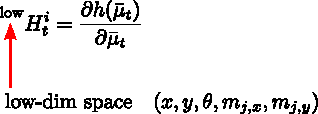
\includegraphics[width=0.4\textwidth]{ekf_slam/jacobian_observation.pdf}
        \end{center}
        %
        % \begin{equation*}
        %     \prescript{\text{low}}{}{H^{i}_{t}} = \frac{\partial h(\bar{\mu}_t)}{\partial \bar{\mu}_t}
        % \end{equation*}
        % \begin{equation*}
        %     \text{low-dim space} \quad (x, y, \theta, \map_{j,x}, \map_{j,y})
        % \end{equation*}

        We are only interested in the 5-dimension related with the observation.

    \end{itemize}
\end{frame}

\begin{frame}
    \frametitle{Jacobian for the Observation}
    \note{Información extraída de https://www.youtube.com/watch?v=X30sEgIws0g}
    \note{Información extraída de https://www.ipb.uni-bonn.de/html/teaching/photo12-2021/2021-pho2-16-ekf-slam.pptx.pdf}

    \begin{itemize}
        \item Based on
        \begin{align*}
            \delta &= 
            \begin{bmatrix}
                \delta_x \\
                \delta_y
            \end{bmatrix}
            = \begin{bmatrix}
                \bar{\mu}_{j,x} - \bar{\mu}_{t,x} \\
                \bar{\mu}_{j,y} - \bar{\mu}_{t,y}
            \end{bmatrix}\\
            q &= \delta^T \delta\\
            \hat{z}^i_t &= 
            \begin{bmatrix}
                \sqrt{q} \\
                \text{atan2}(\delta_y, \delta_x) - \bar{\mu}_{t,\theta}
            \end{bmatrix}
        \end{align*}    
        \item Compute the Jacobian
        \begin{align*}
            \prescript{\text{low}}{}{H^{i}_{t}} &= \frac{\partial h(\bar{\mu}_t)}{\partial \bar{\mu}_t}\\
            &= \begin{bmatrix}
                \frac{\partial \sqrt{q}}{\partial x} & \frac{\partial \sqrt{q}}{\partial y} & \cdots \\
                \frac{\partial \text{atan2}(\ldots)}{\partial x} & \frac{\partial \text{atan2}(\ldots)}{\partial y} & \cdots
            \end{bmatrix}
    \end{align*} 
    \end{itemize}

\end{frame}

\begin{frame}
    \frametitle{The first component}
    \note{Información extraída de https://www.youtube.com/watch?v=X30sEgIws0g}
    \note{Información extraída de https://www.ipb.uni-bonn.de/html/teaching/photo12-2021/2021-pho2-16-ekf-slam.pptx.pdf}

    \begin{itemize}
        \item Based on
        \begin{align*}
            \delta &= 
            \begin{bmatrix}
                \delta_x \\
                \delta_y
            \end{bmatrix}
            = \begin{bmatrix}
                \bar{\mu}_{j,x} - \bar{\mu}_{t,x} \\
                \bar{\mu}_{j,y} - \bar{\mu}_{t,y}
            \end{bmatrix}\\
            q &= \delta^T \delta\\
            \hat{z}^i_t &= 
            \begin{bmatrix}
                \sqrt{q} \\
                \text{atan2}(\delta_y, \delta_x) - \bar{\mu}_{t,\theta}
            \end{bmatrix}
        \end{align*}    
    
        \item We obtain (by applying the chain rule)
        \begin{align*}
            \frac{\partial \sqrt{q}}{\partial x}
            &= \frac{1}{2} \frac{1}{\sqrt{q}} 2 \delta_x (-1)\\
            &= \frac{1}{q} \left(-\sqrt{q} \delta_x \right)
        \end{align*} 
    \end{itemize}

\end{frame}

\begin{frame}
    \frametitle{Jacobian for the Observation}
    \note{Información extraída de https://www.youtube.com/watch?v=X30sEgIws0g}
    \note{Información extraída de https://www.ipb.uni-bonn.de/html/teaching/photo12-2021/2021-pho2-16-ekf-slam.pptx.pdf}

    \begin{itemize}
        \item Based on
        \begin{align*}
            \delta &= 
            \begin{bmatrix}
                \delta_x \\
                \delta_y
            \end{bmatrix}
            = \begin{bmatrix}
                \bar{\mu}_{j,x} - \bar{\mu}_{t,x} \\
                \bar{\mu}_{j,y} - \bar{\mu}_{t,y}
            \end{bmatrix}\\
            q &= \delta^T \delta\\
            \hat{z}^i_t &= 
            \begin{bmatrix}
                \sqrt{q} \\
                \text{atan2}(\delta_y, \delta_x) - \bar{\mu}_{t,\theta}
            \end{bmatrix}
        \end{align*}

        \item Compute the Jacobian
        
        \begin{align*}
            \prescript{\text{low}}{}{H^{i}_{t}} &= \frac{\partial h(\bar{\mu}_t)}{\partial \bar{\mu}_t}\\
            &= \frac{1}{q}
            \begin{bmatrix}
                -\sqrt{q} \delta_x & -\sqrt{q} \delta_y & 0 & \sqrt{q} \delta_x & \sqrt{q} \delta_y\\
                \delta_y & -\delta_x & -q & -\delta_y & \delta_x
            \end{bmatrix}
        \end{align*}
    \end{itemize}

\end{frame}

\begin{frame}
    \frametitle{Jacobian for the Observation}
    \note{Información extraída de https://www.youtube.com/watch?v=X30sEgIws0g}
    \note{Información extraída de https://www.ipb.uni-bonn.de/html/teaching/photo12-2021/2021-pho2-16-ekf-slam.pptx.pdf}

    \small

    \begin{itemize}
        \item Use the computed Jacobian
        \begin{align*}
            \prescript{\text{low}}{}{H^{i}_{t}} &= \frac{\partial h(\bar{\mu}_t)}{\partial \bar{\mu}_t}\\
            &= \frac{1}{q}
            \begin{bmatrix}
                -\sqrt{q} \delta_x & -\sqrt{q} \delta_y & 0 & \sqrt{q} \delta_x & \sqrt{q} \delta_y\\
                \delta_y & -\delta_x & -q & -\delta_y & \delta_x
            \end{bmatrix}
        \end{align*}
    
        \item Map it to the high dimensional space
        \begin{equation*}
            H^{i}_{t} = \prescript{\text{low}}{}{H^{i}_{t}} F_{x,j}
        \end{equation*}
        \begin{equation*}
            F_{x,j} =
            \begin{bNiceMatrix}[margin = 3 pt]
                1 & 0 & 0 & 0 \cdots 0 & 0 & 0 & 0 \cdots 0 \\
                0 & 1 & 0 & 0 \cdots 0 & 0 & 0 & 0 \cdots 0 \\
                0 & 0 & 1 & 0 \cdots 0 & 0 & 0 & 0 \cdots 0 \\
                0 & 0 & 0 & 0 \cdots 0 & 1 & 0 & 0 \cdots 0 \\
                0 & 0 & 0 & 0 \cdots 0 & 0 & 1 & 0 \cdots 0
                \CodeAfter
                \UnderBrace{5-4}{5-4}{2(j-1)}
                \UnderBrace{5-7}{5-7}{2(N-j)}
            \end{bNiceMatrix}
        \end{equation*} 
    \end{itemize}
\end{frame}

\begin{frame}
    \frametitle{Extended Kalman Filter Algorithm}
    \note{Información extraída de https://www.youtube.com/watch?v=X30sEgIws0g}
    \note{Información extraída de https://www.ipb.uni-bonn.de/html/teaching/photo12-2021/2021-pho2-16-ekf-slam.pptx.pdf}
    
    \begin{algorithmic}[1]
    \Procedure{ExtendedKalmanFilter}{$\mu_{t-1}, \covariance_{t-1}, \controlCommand_{t}, \observation_{t}$}
        \State $\overline{\mu}_{t} = \motionModelFunction{\controlCommand_{t}, \mu_{t-1}}$
        \State $\overline{\covariance}_{t} = \motionModelJacobian_{t} \covariance_{t-1} \motionModelJacobian_{t}^{\top}+\motionParametersCovariance_{t}$
        \Statex
        \State $\alert{\kalmanGain_{t} = \overline{\covariance}_{t} \observationModelJacobian_{t}^{\top} (\observationModelJacobian_{t} \overline{\covariance}_{t}  \observationModelJacobian_{t} + \observationModelCovariance_{t})^{-1}}$
        \State $\alert{\mu_{t} = \overline{\mu}_{t} + \kalmanGain_{t} (\observation_{t} - \observationModelFunction{\overline{\mu}_{t}})}$
        \State $\alert{\covariance_{t} =  (I - \kalmanGain_{t} \observationModelJacobian_{t}) \overline{\covariance}_{t}}$
        \State \Return $\mu_{t}, \covariance_{t}$
    \EndProcedure
    \end{algorithmic}
\end{frame}

\begin{frame}
    \frametitle{EKF SLAM - Correction (1/2)}
    \note{Información extraída de https://www.youtube.com/watch?v=X30sEgIws0g}
    \note{Información extraída de https://www.ipb.uni-bonn.de/html/teaching/photo12-2021/2021-pho2-16-ekf-slam.pptx.pdf}

    \begin{algorithmic}[1]
        \Procedure{EKF\_SLAM\_Correction}{}
        \State $Q_t = \begin{bmatrix} \sigma_r^2 & 0 \\ 0 & \sigma_\theta^2 \end{bmatrix}$ \Comment{Measurement noise covariance}
        \For {all observed features $\observation_i^t = (r_i^t, \phi_i^t)^{\top}$}
            \State $j = c_i^t$ \Comment{data association somehow}
            \If{landmark $j$ never seen before}
                \State $\begin{bmatrix} \bar{\mu}_{j,x} \\ \bar{\mu}_{j,y} \end{bmatrix} = 
                       \begin{bmatrix} \bar{\mu}_{t,x} \\ \bar{\mu}_{t,y} \end{bmatrix} + 
                       \begin{bmatrix} r_i^t \cos(\phi_i^t + \bar{\mu}_{t,\theta}) \\ r_i^t \sin(\phi_i^t + \bar{\mu}_{t,\theta}) \end{bmatrix}$
                \Comment{Initialize new landmark position}
            \EndIf
            \State $\delta = \begin{bmatrix} \delta_x \\ \delta_y \end{bmatrix} = 
                   \begin{bmatrix} \bar{\mu}_{j,x} - \bar{\mu}_{t,x} \\ \bar{\mu}_{j,y} - \bar{\mu}_{t,y} \end{bmatrix}$
            \State $q = \delta^T \delta$
            \State $\hat{z}_i^t = \begin{bmatrix} \sqrt{q} \\ \operatorname{atan2}(\delta_y, \delta_x) - \bar{\mu}_{t,\theta} \end{bmatrix}$
                   \Comment{Predicted measurement}
        \algstore{ekf_slam_algorithm_break} % guarda el estado del argoritmo para que este pueda continuar en otro lugar
    \end{algorithmic}
\end{frame}

\begin{frame}
    \frametitle{EKF SLAM - Correction (2/2)}
    \note{Información extraída de https://www.youtube.com/watch?v=X30sEgIws0g}
    \note{Información extraída de https://www.ipb.uni-bonn.de/html/teaching/photo12-2021/2021-pho2-16-ekf-slam.pptx.pdf}

    \begin{algorithmic}[1]
        \algrestore{ekf_slam_algorithm_break} % continua el algoritmo de antes
        \State $F_{x,j} =
        \begin{bNiceMatrix}[margin = 3 pt]
            1 & 0 & 0 & 0 \cdots 0 & 0 & 0 & 0 \cdots 0 \\
            0 & 1 & 0 & 0 \cdots 0 & 0 & 0 & 0 \cdots 0 \\
            0 & 0 & 1 & 0 \cdots 0 & 0 & 0 & 0 \cdots 0 \\
            0 & 0 & 0 & 0 \cdots 0 & 1 & 0 & 0 \cdots 0 \\
            0 & 0 & 0 & 0 \cdots 0 & 0 & 1 & 0 \cdots 0
            \CodeAfter
            \UnderBrace{5-4}{5-4}{2j-2}
            \UnderBrace{5-7}{5-7}{2N-2j}
        \end{bNiceMatrix}$ \Comment{Jacobian of state mapping}
        \Statex
        \Statex
        \State $H_t^i = \frac{1}{q} \begin{bmatrix}
            -\sqrt{q} \delta_x & -\sqrt{q} \delta_y & 0 & \sqrt{q} \delta_x & \sqrt{q} \delta_y\\
            \delta_y & -\delta_x & -q & -\delta_y & \delta_x
        \end{bmatrix} F_{x,j}$ \Comment{Measurement Jacobian}
            
        \State $K_t^i = \bar{\Sigma}_t H_t^{i\top}(H_t^i \bar{\Sigma}_t H_t^{i\top} + Q_t)^{-1}$ \Comment{Kalman gain}
        \State $\bar{\mu}_t = \bar{\mu}_t + K_t^i(\observation_t^i - \hat{z}_t^i)$ \Comment{State update}
        \State $\bar{\Sigma}_t = (I - K_t^i H_t^i) \bar{\Sigma}_t$ \Comment{Covariance update}
        \EndFor
        \State $\mu_t = \bar{\mu}_t$ \Comment{Final state estimate}
        \State $\Sigma_t = \bar{\Sigma}_t$ \Comment{Final covariance estimate}
        \State \Return $\mu_t, \Sigma_t$ \Comment{Return updated state and covariance}
        \EndProcedure
    \end{algorithmic}
\end{frame}

\begin{frame}
    \frametitle{Implementation Notes}
    \note{Información extraída de https://www.youtube.com/watch?v=X30sEgIws0g}
    \note{Información extraída de https://www.ipb.uni-bonn.de/html/teaching/photo12-2021/2021-pho2-16-ekf-slam.pptx.pdf}

    \begin{itemize}
        \item Measurement update in a single step requires only one full belief update
        \item Always normalize angular components to be in $[-\pi,\pi]$. Otherwise this can screw up the jacobians.
        \item May not need to create $F$ matrices explicitly \note{you can manipulate the covarince matrix elements directly}
    \end{itemize}

    \note{As we describe the pseudo-code we need one full belief update for each observed landmark indepently. In Practivce, we can do a full belief update using all the landmarks that currently observed to speed up computation.}

\end{frame}

\begin{frame}
    \frametitle{Loop Closing}
    \note{Información extraída de https://www.youtube.com/watch?v=X30sEgIws0g}
    \note{Información extraída de https://www.ipb.uni-bonn.de/html/teaching/photo12-2021/2021-pho2-16-ekf-slam.pptx.pdf}

    \begin{itemize}
    \item Loop closing means revisiting (and recognizing) an already mapped area
    \item Data association under
    \begin{itemize}
        \item high ambiguity
        \item possible environment symmetries
    \end{itemize}
    \item Uncertainties collapse after a loop closure (whether the closure was correct or not)
    \item \alert{Wrong loop closures lead to filter divergence!}
    \end{itemize}
\end{frame}

\begin{frame}
    \frametitle{Before the Loop Closure}
    \note{Información extraída de https://www.youtube.com/watch?v=X30sEgIws0g}
    \note{Información extraída de https://www.ipb.uni-bonn.de/html/teaching/photo12-2021/2021-pho2-16-ekf-slam.pptx.pdf}

    \begin{center}
        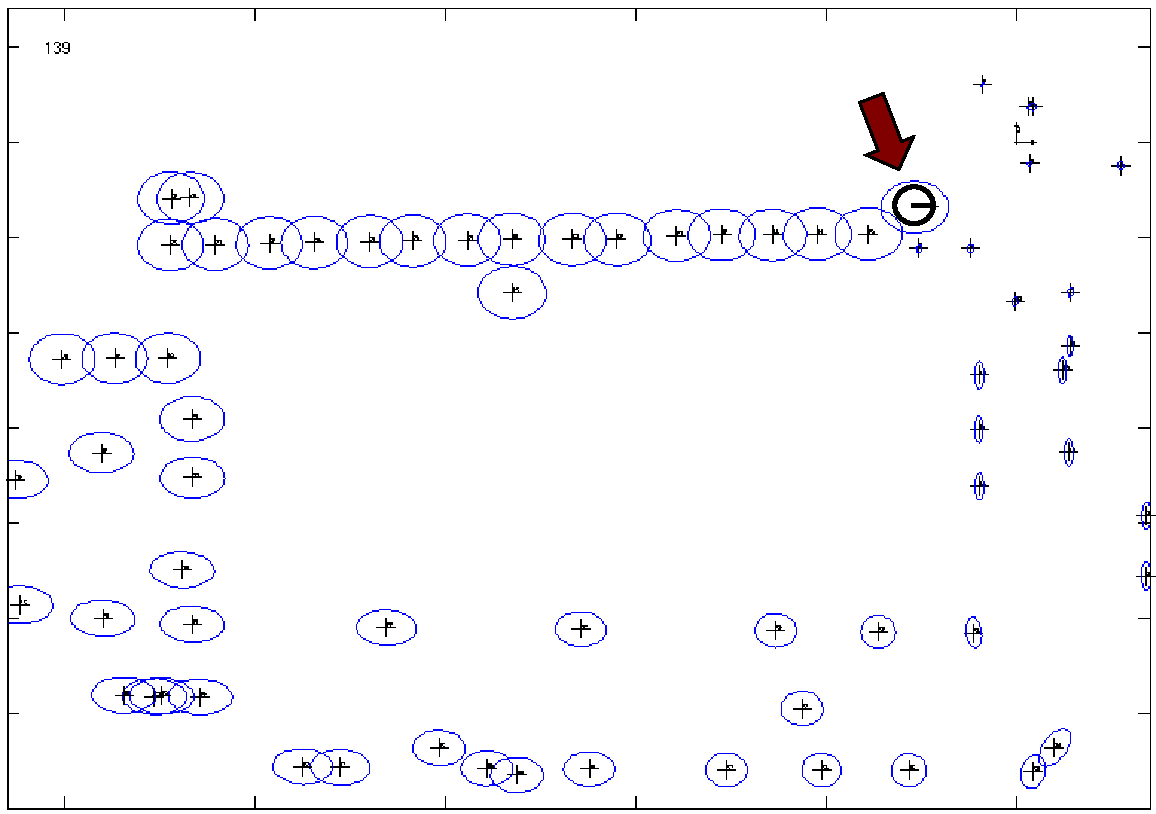
\includegraphics[width=0.6\textwidth]{ekf_slam/ekf_slam_loop_closure_before.pdf}
    \end{center}
\end{frame}

\begin{frame}
    \frametitle{After the Loop Closure}
    \note{Información extraída de https://www.youtube.com/watch?v=X30sEgIws0g}
    \note{Información extraída de https://www.ipb.uni-bonn.de/html/teaching/photo12-2021/2021-pho2-16-ekf-slam.pptx.pdf}

    \begin{center}
        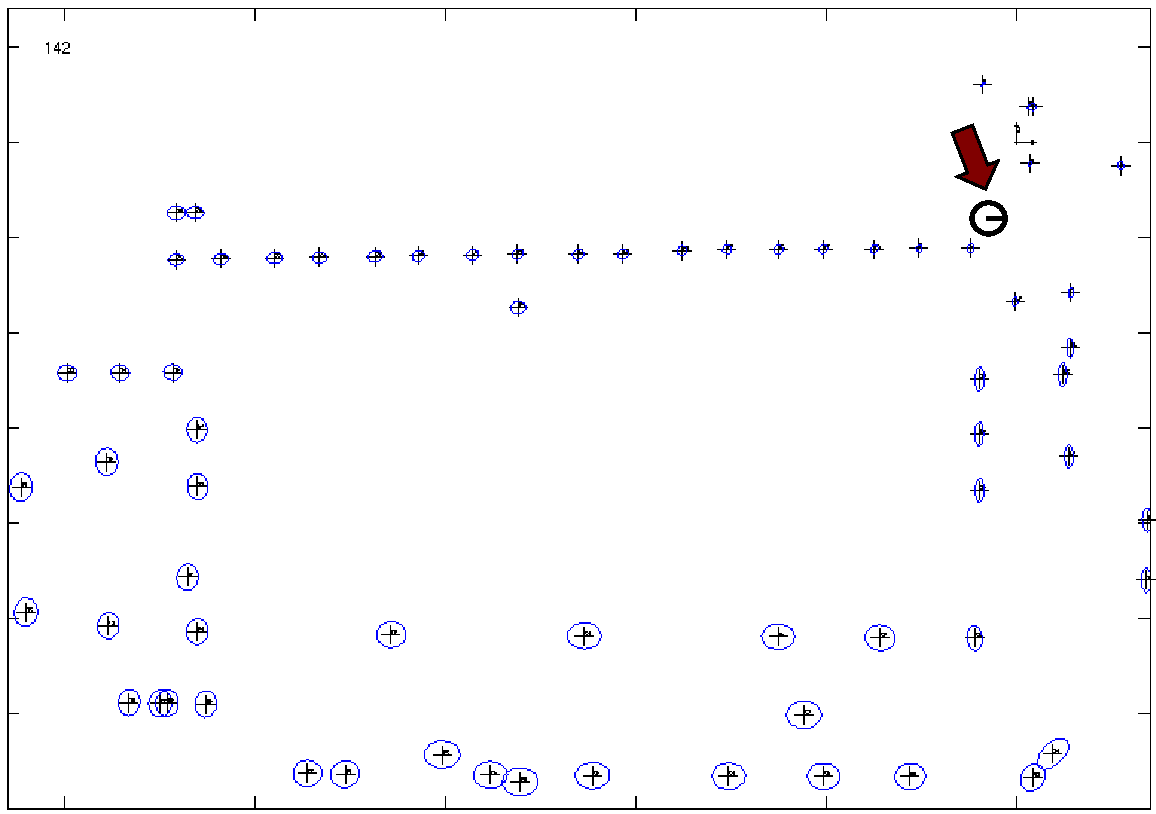
\includegraphics[width=0.6\textwidth]{ekf_slam/ekf_slam_loop_closure_after.pdf}
    \end{center}
\end{frame}

\begin{frame}
    \frametitle{Loop Closing}
    \note{Información extraída de https://www.youtube.com/watch?v=X30sEgIws0g}
    \note{Información extraída de https://www.ipb.uni-bonn.de/html/teaching/photo12-2021/2021-pho2-16-ekf-slam.pptx.pdf}

    \begin{itemize}
    \item Loop closing reduces the uncertainty in robot and landmark estimates
    \item This can be exploited when exploring an environment for the sake of better (e.g. more accurate) maps
    \item Wrong loop closures lead to filter divergence
    \end{itemize}
\end{frame}

\begin{frame}
    \frametitle{EKF SLAM Correlations}
    \note{Información extraída de https://www.youtube.com/watch?v=X30sEgIws0g}
    \note{Información extraída de https://www.ipb.uni-bonn.de/html/teaching/photo12-2021/2021-pho2-16-ekf-slam.pptx.pdf}

    \begin{itemize}
        \item In the limit, the landmark estimates become fully correlated
    \end{itemize}

    \begin{center}
        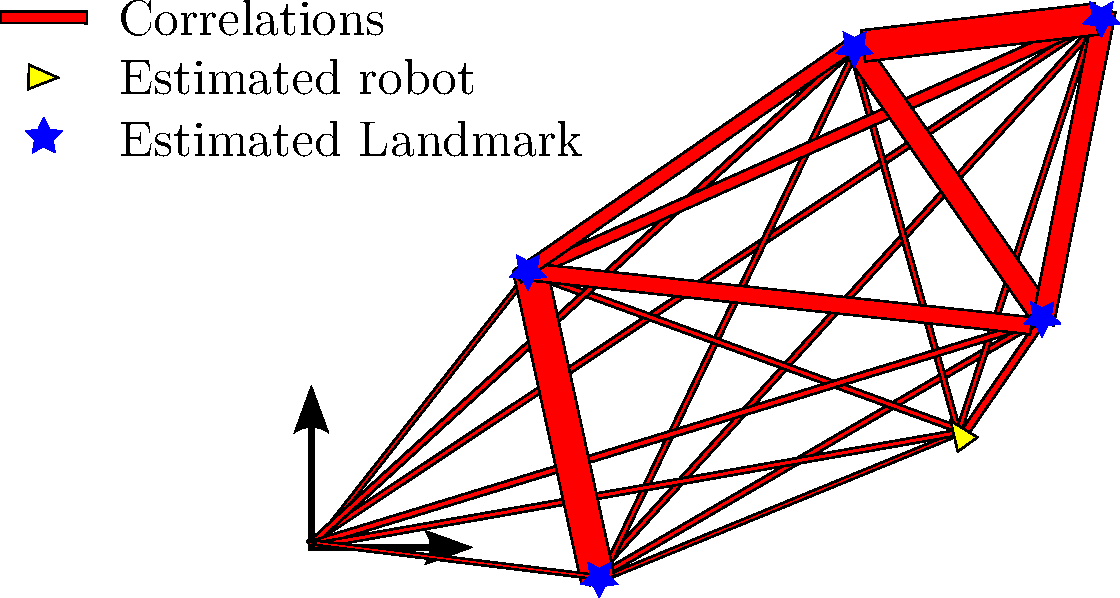
\includegraphics[width=0.45\textwidth]{../images/ekf_slam/ekf_slam_correlations.pdf}
    \end{center}

    \scriptsize

    \begin{itemize}
        \item In the long run all the estimates are fully correlated. All the landmark locations are fully (and strongly) correlated with each other (thick lines) and the pose is correlated with the landmarks in a weaker manner (thin lines).
        \item The Covariance Matrix represents the uncertainty and correlation between different state variables (e.g., robot pose and positions of landmarks). The \textbf{correlation matrix} is the normalized covariance matrix of the posterior estimate.
        \begin{itemize}
            \item Diagonal: Variance (uncertainty) of each variable.
            \item Off-diagonal: Correlation between variables (how errors in one affect another).
        \end{itemize}
    \end{itemize}

    \note{The correlation matrix simply divides the covariance of the two variables by the product of their standard deviations.}
    
\end{frame}

\begin{frame}
    \frametitle{EKF SLAM Correlations}
    \note{Información extraída de https://www.youtube.com/watch?v=X30sEgIws0g}
    \note{Información extraída de https://www.ipb.uni-bonn.de/html/teaching/photo12-2021/2021-pho2-16-ekf-slam.pptx.pdf}

    \begin{center}
        \only<1>{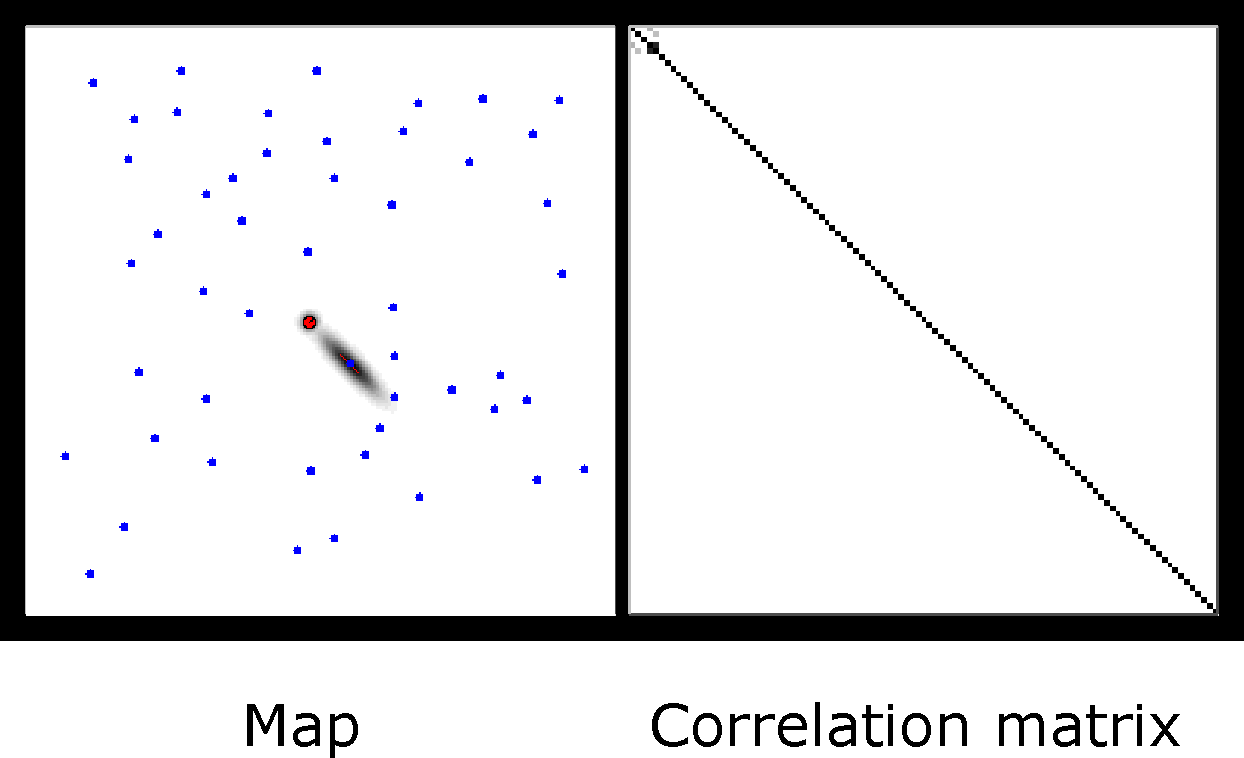
\includegraphics[width=0.8\textwidth]{../images/ekf_slam/ekf_slam_correlation_matrix1.pdf}}
        \only<2>{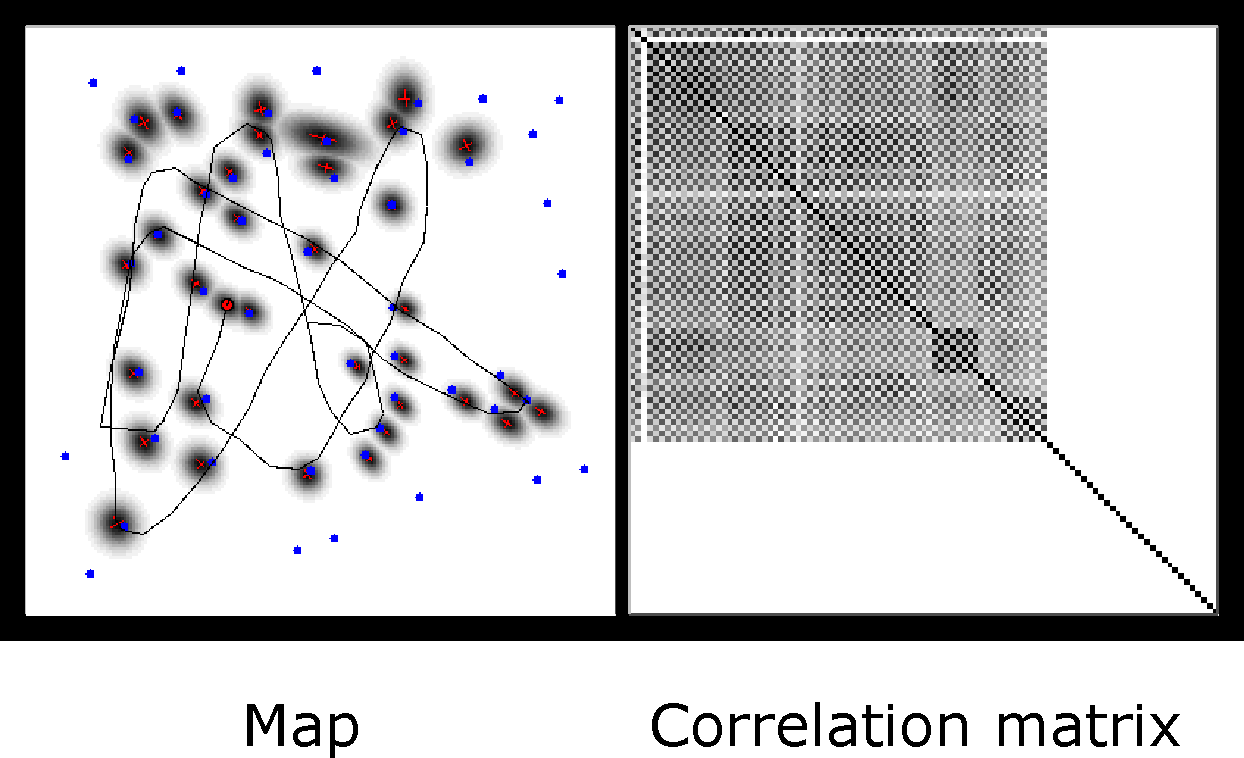
\includegraphics[width=0.8\textwidth]{../images/ekf_slam/ekf_slam_correlation_matrix2.pdf}}
        \only<3>{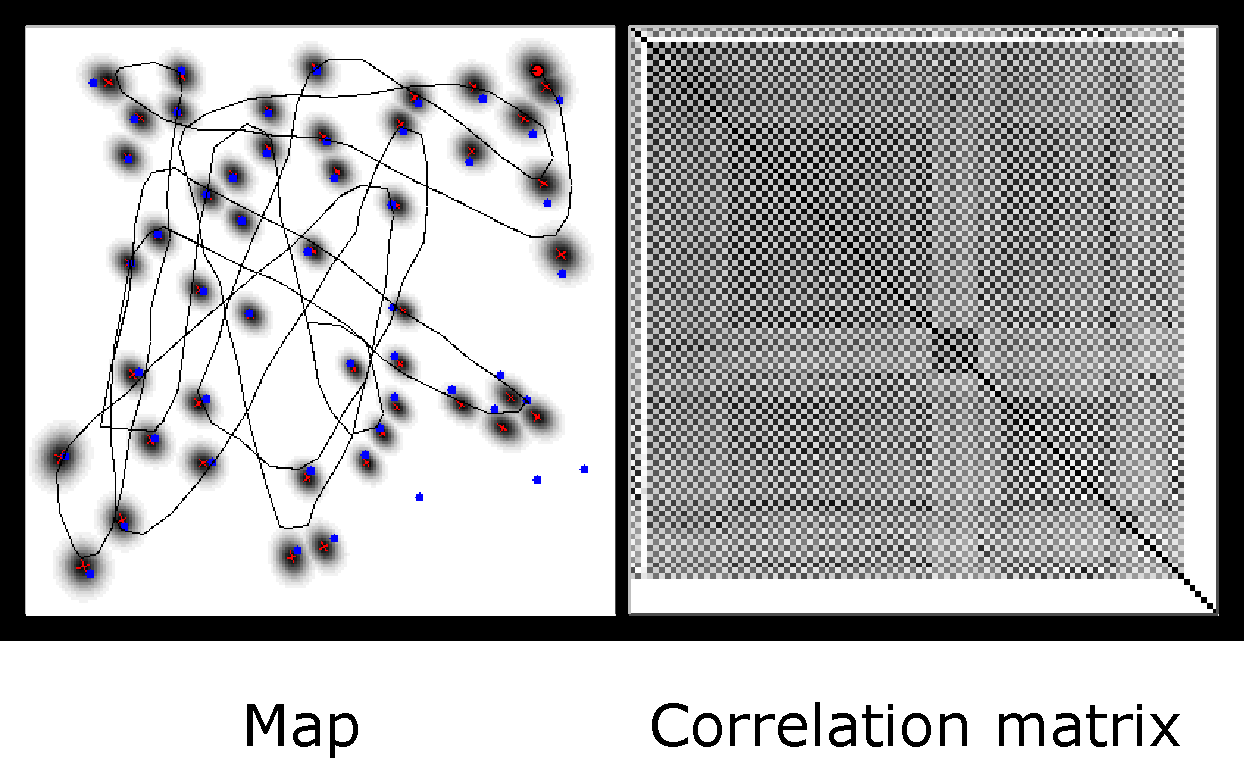
\includegraphics[width=0.8\textwidth]{../images/ekf_slam/ekf_slam_correlation_matrix3.pdf}}
    \end{center}

    \note{The while line (zero values) in the third row and column of the correlation matrix comes from the orientation. This means the robot orientation is not correlated with the lanmarks positions.}

    \note{Note that the correlation matrix looks like a checkboard. This is because, in the map, each landmark has a covariance that is mosly a circle, so the 2x2 landmarks covariance block of the main diagonal of the correlation matrix, off-diagonal elements of such 2x2 block are close to zero.
    On the other hand, for the off-diagonal elements of the correlation matrix, if I would be able to fix the x component location of one landmark, so I could dramatically reduce the uncertainty about the x location of all the other landmarks as well, because through the estimate Iquite of rigitdly connected those landmarks so if I shift one landmark with high uncertainty with zero uncertainty then all the map will shift as well. Therefore, if know the precise x location of a landmark I will know all the x locations of all other landmarks as well but I not learn anything about y.}

\end{frame}

\begin{frame}
    \frametitle{EKF SLAM Correlations}
    \note{Información extraída de https://www.youtube.com/watch?v=X30sEgIws0g}
    \note{Información extraída de https://www.ipb.uni-bonn.de/html/teaching/photo12-2021/2021-pho2-16-ekf-slam.pptx.pdf}

    \begin{itemize}
        \item The correlation between the robot's pose and the landmarks \textbf{cannot} be ignored 
        \item Assuming independence generates too optimistic estimates of the uncertainty
    \end{itemize}

    \note{So if you ignore the correlations you will be too optimistic since this means that you are setting all the other uncertainty values to zero.}

\end{frame}

\begin{frame}
    \frametitle{EKF SLAM Uncertainties}
    \note{Información extraída de https://www.youtube.com/watch?v=X30sEgIws0g}
    \note{Información extraída de https://www.ipb.uni-bonn.de/html/teaching/photo12-2021/2021-pho2-16-ekf-slam.pptx.pdf}

    \begin{itemize}
    \item The \textbf{determinant} of any sub-matrix of the map covariance matrix \textbf{decreases monotonically}
    \item New landmarks are initialized with \textbf{maximum uncertainty}
    \end{itemize}

    \begin{center}
        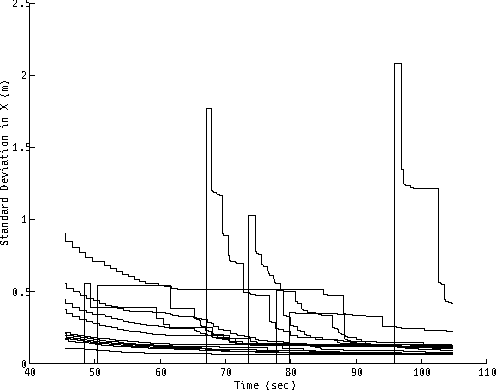
\includegraphics[width=0.5\textwidth]{../images/ekf_slam/landmarks_uncertainty_decrease.pdf} % Replace with actual vectorized image
    \end{center}
\end{frame}

\begin{frame}
    \frametitle{EKF SLAM in the Limit}
    \note{Información extraída de https://www.youtube.com/watch?v=X30sEgIws0g}
    \note{Información extraída de https://www.ipb.uni-bonn.de/html/teaching/photo12-2021/2021-pho2-16-ekf-slam.pptx.pdf}
    
    \begin{itemize}
        \item In the limit, the covariance associated with any single landmark location estimate is determined only by the initial covariance in the vehicle location estimate.
    \end{itemize}

    \begin{center}
        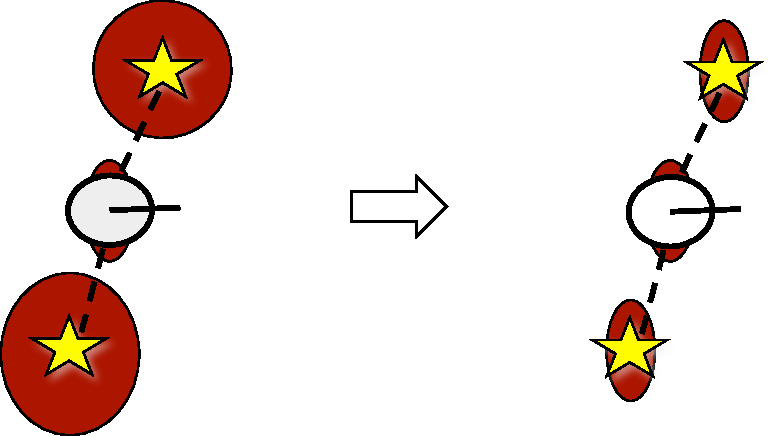
\includegraphics[width=0.6\textwidth]{../images/ekf_slam/ekf_slam_limit.pdf}
    \end{center}

\end{frame}

\begin{frame}
    \frametitle{EKF-SLAM 2D Example}
    \note{Vídeo extraído de https://youtu.be/xXo5oBYnuxE?si=VGVFflbAgcABIIVf}
    \note{https://github.com/taihup/slam_ekf_ros2}
        
    \begin{center}
    \movie[poster,loop,showcontrols]{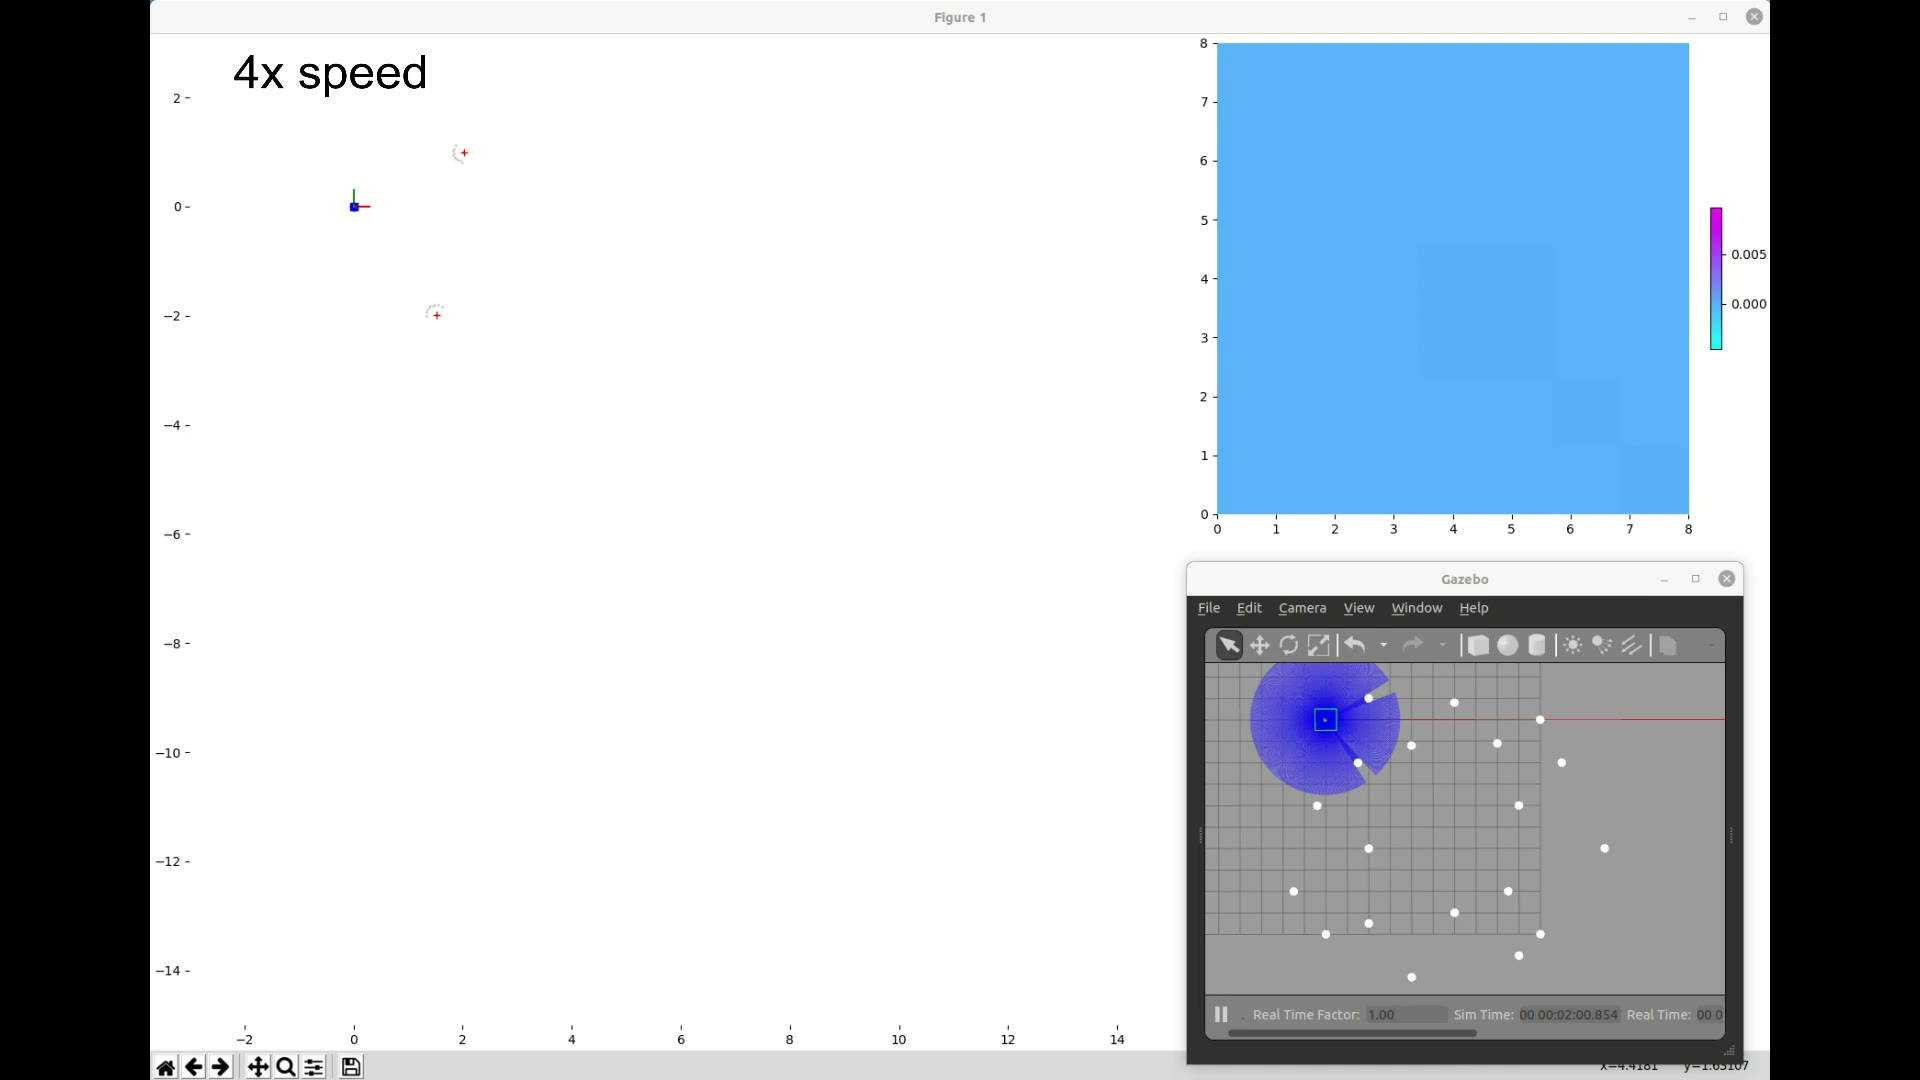
\includegraphics[width=0.9\columnwidth]{./images/ekf_slam/ekf_slam_2d_video.jpg}}{./videos/ekf_slam_2d.mp4}
    \end{center}

    \note{The covariance matrix is shown in the upper-left corner.}

\end{frame}

\begin{frame}
    \frametitle{EKF SLAM Complexity}
    \note{Información extraída de https://www.youtube.com/watch?v=X30sEgIws0g}
    \note{Información extraída de https://www.ipb.uni-bonn.de/html/teaching/photo12-2021/2021-pho2-16-ekf-slam.pptx.pdf}

    \begin{itemize}
    \item Cubic complexity w.r.t. measurement dimensionality \note{and not w.r.t the whole state, this is because you are only observing small number of landmark and not the whole map.}
    \item Cost per step: $O(n^2)$ (dominated by number of landmarks)
    \item Memory consumption: $O(n^2)$
    \item Computationally intractable for large maps!
    \end{itemize}
\end{frame}

\begin{frame}
    \frametitle{EKF SLAM Summary}
    \note{Información extraída de https://www.youtube.com/watch?v=X30sEgIws0g}
    \note{Información extraída de https://www.ipb.uni-bonn.de/html/teaching/photo12-2021/2021-pho2-16-ekf-slam.pptx.pdf}

    \begin{itemize}
    \item First probabilistic SLAM approach using EKF
    \item Convergence proof for the linear Gaussian case
    \item Can diverge if non-linearities are large
    \item The smaller the noise the better
    \item Unimodal (Gaussian) estimates only \note{EKF can not handle multimodal uncertainty. Eg: I cannot say either the landmark is here or there but I don't exatly know. Particle filter can!}
    \item Successful in medium-scale scenes
    \item Used for short-term estimates (VO)
    \item Approximations exists to reduce the computational complexity
    
    \end{itemize}
\end{frame}

\begin{frame}
    \frametitle{Literature}
    \note{Información extraída de https://www.youtube.com/watch?v=X30sEgIws0g}
    \note{Información extraída de https://www.ipb.uni-bonn.de/html/teaching/photo12-2021/2021-pho2-16-ekf-slam.pptx.pdf}

    \begin{itemize}
    \item Thrun et al.: "Probabilistic Robotics", Chapter 10
    \end{itemize}
\end{frame}

	\section{Factor-Graph}
	\begin{frame}
    \frametitle{Graph-SLAM}
    
    Graph-SLAM: Construct a graph and find a configuration of nodes that minimizes the error introduced by constraints (edges)
    
    \begin{itemize}
    \item A graph is used to represent the problem.
    \item The nodes represent poses or locations of landmarks.
    \item Edges are landmark observations or odometry measurements
    \item Minimization optimizes robot poses and landmark placement
    \item Observing previously viewed areas generates constraints in the graph
    \end{itemize}
    
    \begin{figure}
    \subfloat[]
    {
    \fbox{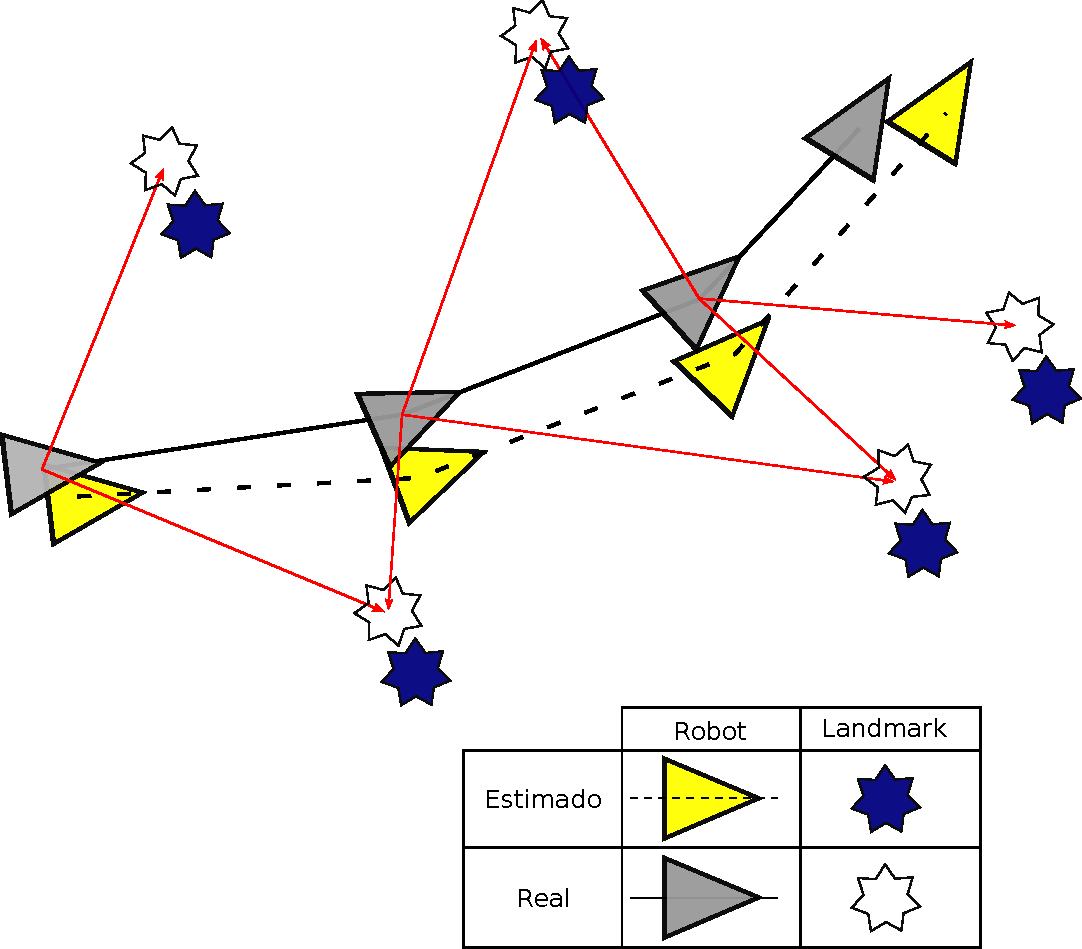
\includegraphics[width=0.25\textwidth]{images/slam-landmarks.pdf}}
    }\hspace{1em}
    \subfloat[]
    {
    \fbox{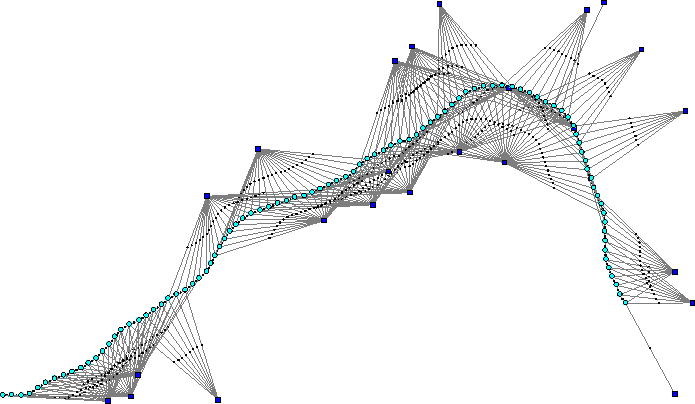
\includegraphics[width=0.375\textwidth]{images/factor_graph.pdf}}
    }
    \end{figure}
    
    \end{frame}
    
    \begin{frame}
    \frametitle{Factor-Graph}
    \note{Information taken from https://youtu.be/uuiaqGLFYa4}
    
    \begin{block}{Factor-Graph}
    A Factor-graph is a mathematical term, a bipartite graph representing the factorization of a function. This means that we can take a function, for example, $g(.)$ and decompose it by the product of functions $f(.)$,
    
    \begin{equation*}
    g(X_{1}, \dots, X_{n}) = \prod_{i} f_{i}(S_{i}) \quad \text{con} \quad S_{i} \subseteq \{ X_{1},\dots, X_{n} \}
    \end{equation*}
    \end{block}
    
    \begin{figure}[!h]
    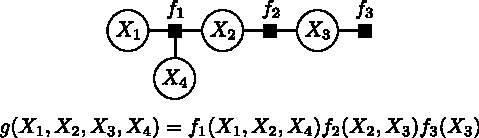
\includegraphics[width=0.7\textwidth]{images/factor_graph_example.pdf}
    \end{figure}
    
    \note{For example, if the function g depends on 10 variables, we can decompose it into the product of several functions f, where each function f depends on a subset of those variables.}
    
    \end{frame}
    
    \begin{frame}
    \frametitle{Factor-Graph}
    \note{Information taken from https://youtu.be/uuiaqGLFYa4}
    
    \begin{itemize}
    \item Factor-graphs allow us to represent a joint probability distribution (a distribution that governs all variables) as a product of smaller probabilities (which depend on a smaller number of variables).
    \item Like Bayes networks or Markov networks, we can use Factor-graphs to describe how variables depend on each other. And we can run different algorithms on these Factor-graphs to efficiently infer information.
    \item An example of an algorithm that works on a Factor-graph is the Sum-Product Algorithm for computing marginal distributions (distributions that only depend on a subset of variables).
    \item In the context of robotics, Factor-graphs are used to specify least squares problems. The factor graph allows us to represent how certain states depend on or are related to each other based on the information we have from sensor measurements (stored in the factors).
    \end{itemize}
    
    \note{For example, if function g depends on 10 variables, we can decompose it into the product of several functions f, where each function f depends on a subset of those variables.}
    
    \end{frame}
    
    \begin{frame}
    \frametitle{Graph-based SLAM using Pose-Graph}
    \note{Information taken from https://youtu.be/uHbRKvD8TWg}
    
    \begin{itemize}
    \item The constraints connect the robot's poses as it moves.
    \item The constraints are noisy.
    \end{itemize}
    
    \begin{figure}[!h]
    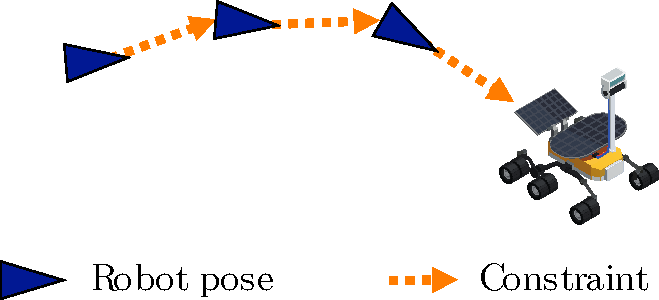
\includegraphics[width=0.7\textwidth]{images/pose_graph_example.pdf}
    \end{figure}
    
\end{frame}

\begin{frame}
    \frametitle{Graph-based SLAM using Pose-Graph}
    \note{Information taken from https://youtu.be/uHbRKvD8TWg}
   
    \begin{itemize}
    \item By observing previously seen areas, restrictions are generated between non-consecutive poses (\emph{Loop Closure})
    \end{itemize}
   
    \begin{figure}[!h]
    \includegraphics[width=0.4\textwidth]{images/pose_graph_loop_example.pdf}
    \end{figure}
   
   \end{frame}
   
   \begin{frame}[fragile]
    \frametitle{2D Pose-Graph with LiDAR}
    \note{Video taken from https://youtu.be/E6IvbjZA7Ao}
   
    \begin{center}
   \movie[loop]{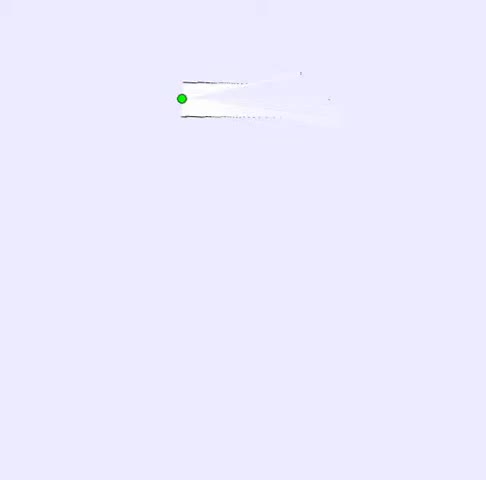
\includegraphics[width=0.5\columnwidth]{./images/pose_graph_2d_video.jpg}}{./videos/pose_graph_2d.mp4}
   \end{center}
   
   \end{frame}
   
   \begin{frame}
   \frametitle{Graph-based SLAM using Pose-Graph}
   \note{Information taken from https://youtu.be/uHbRKvD8TWg}
   
   \begin{columns}
   \begin{column}{0.5\textwidth}
   \begin{itemize}
   \item<1-2> Each node is a robot pose along with its laser measurement (there are no landmarks)
   \item<1-2> Each edge corresponds to a spatial constraint between the nodes it relates. \item<3-> Once we have the graph, we obtain the most probable map by correcting the nodes
    \item<4-> like this...
    \item<5> We draw the map based on the corrected poses
    \end{itemize}
    \end{column}
    \begin{column}{0.5\textwidth} %%<--- here
    \only<1>{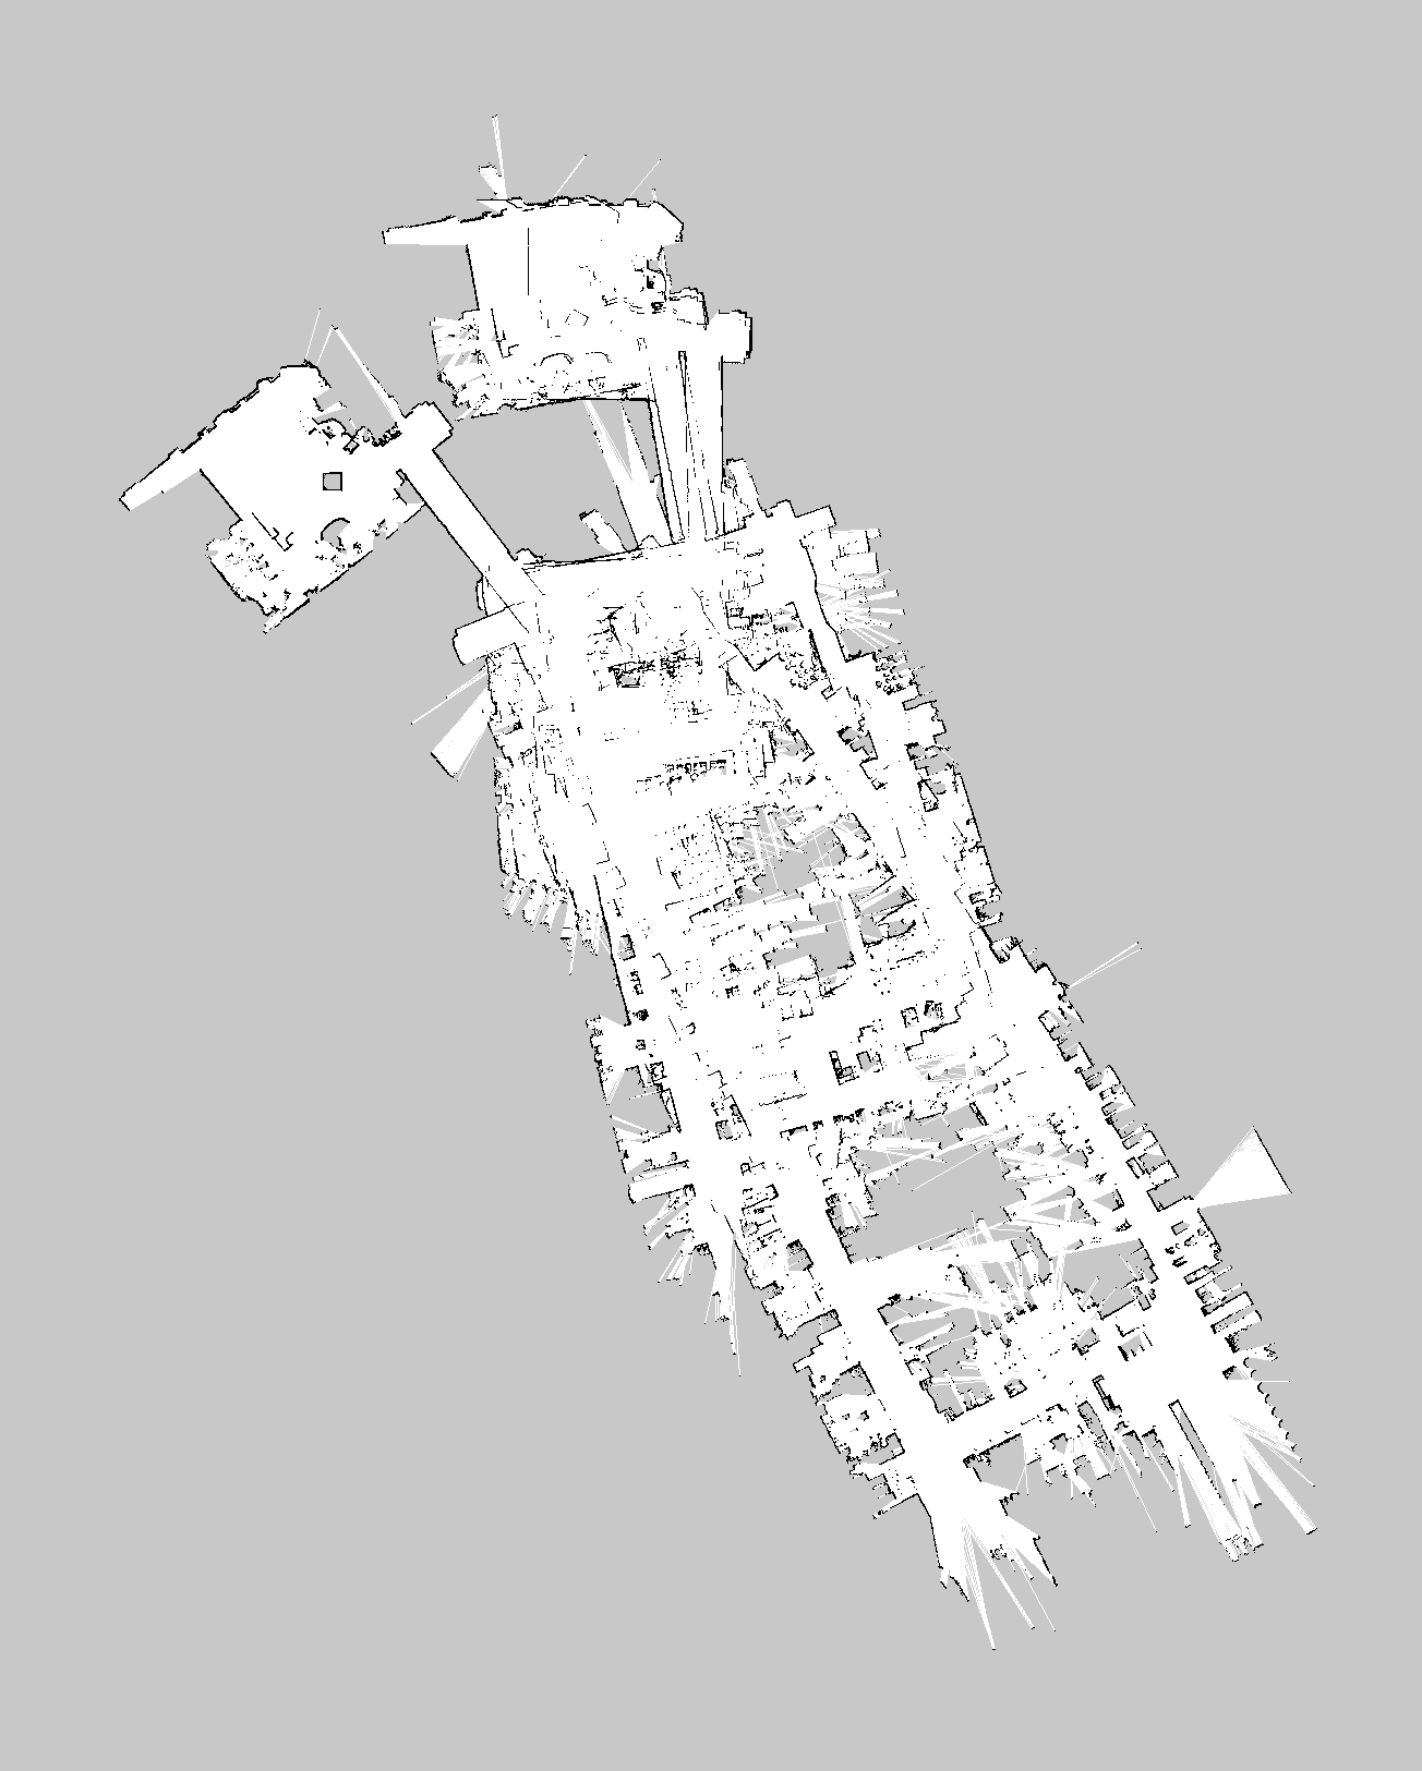
\includegraphics[width=0.7\textwidth]{images/pose_graph_map.png}}
    \only<2>{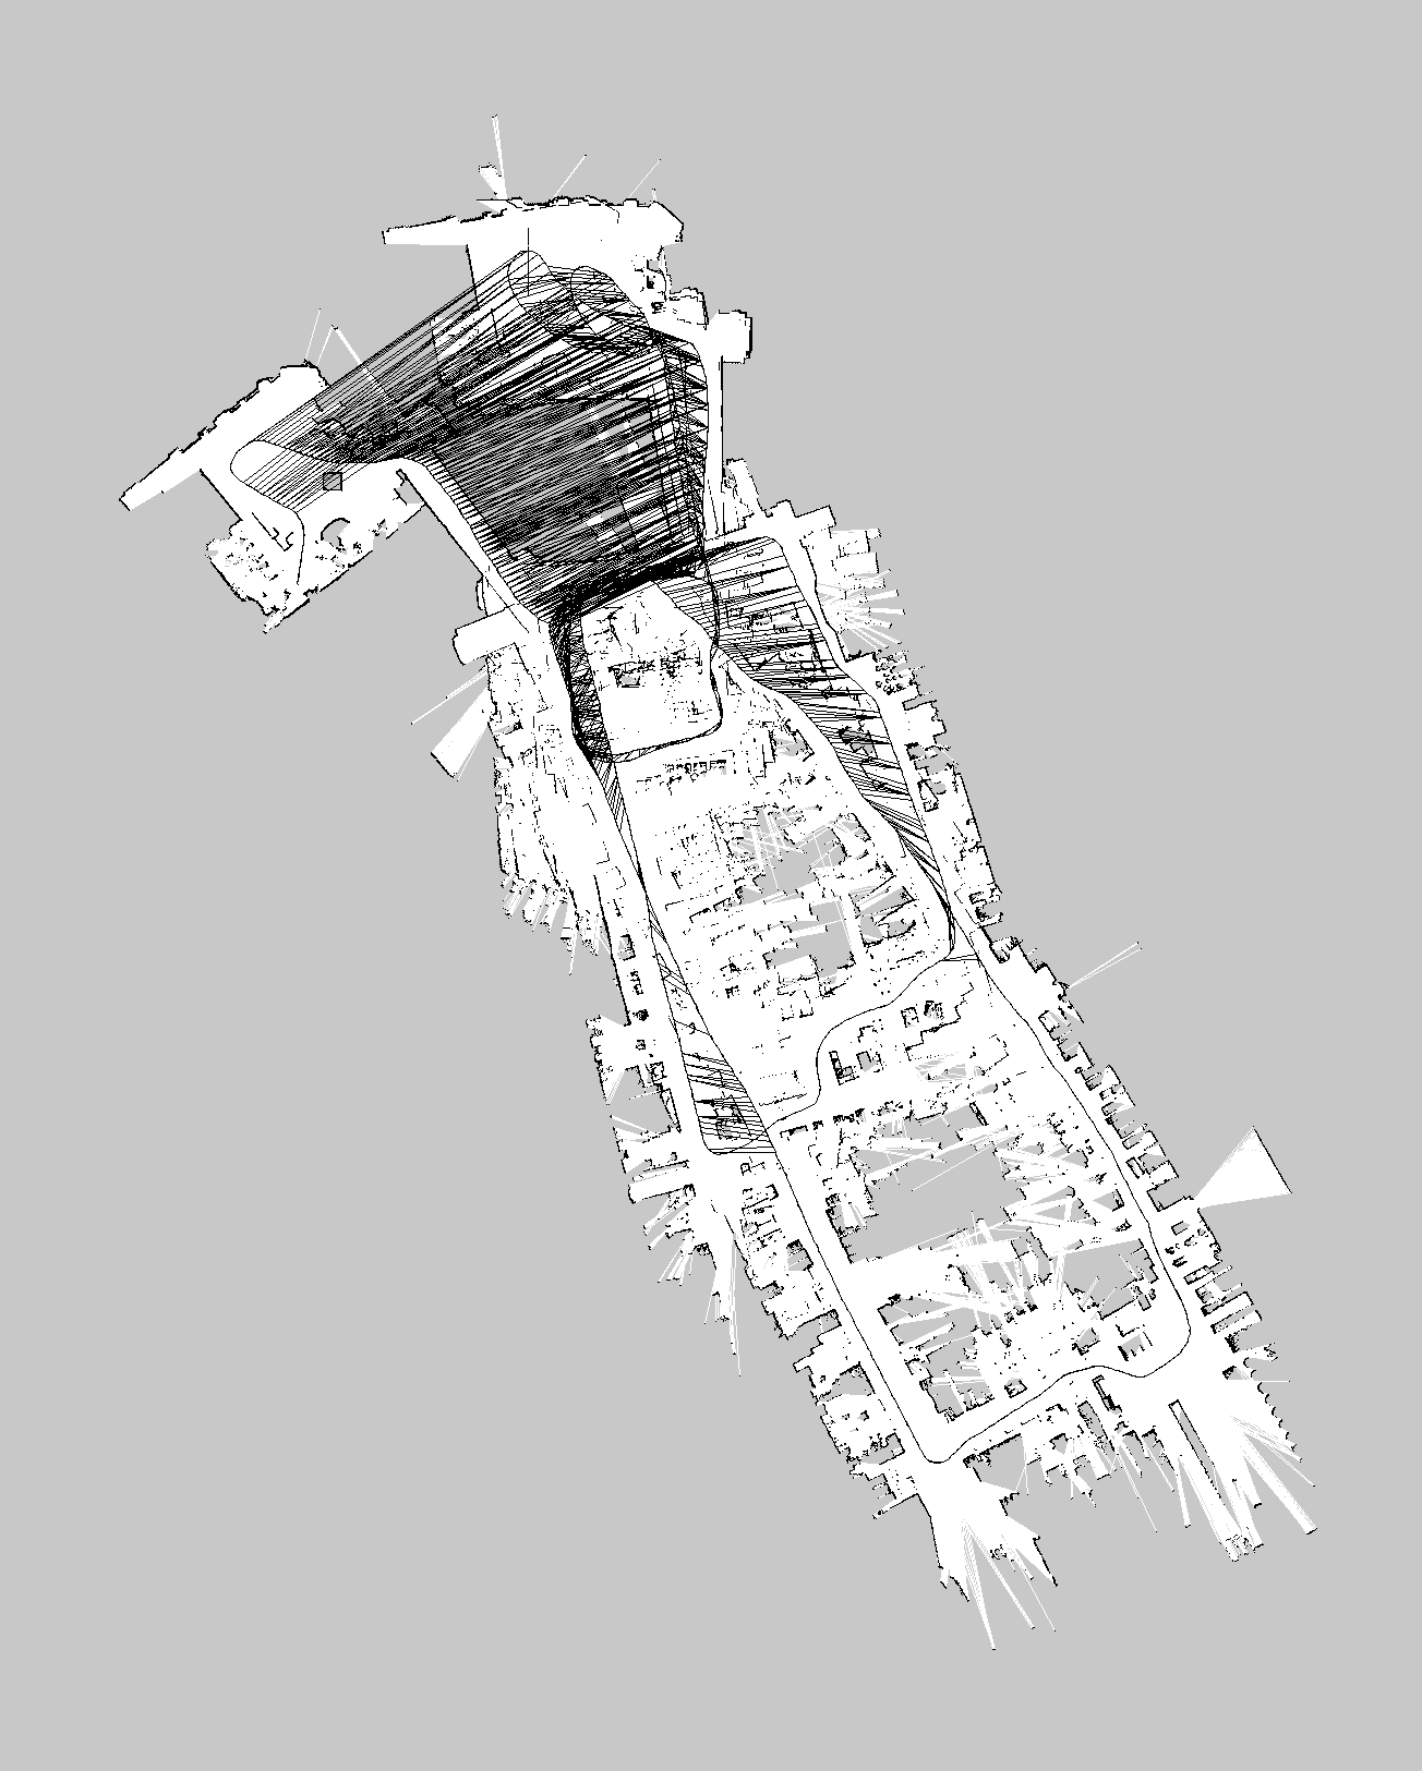
\includegraphics[width=0.7\textwidth]{images/pose_graph_constraints_with_map.png}}
    \only<3>{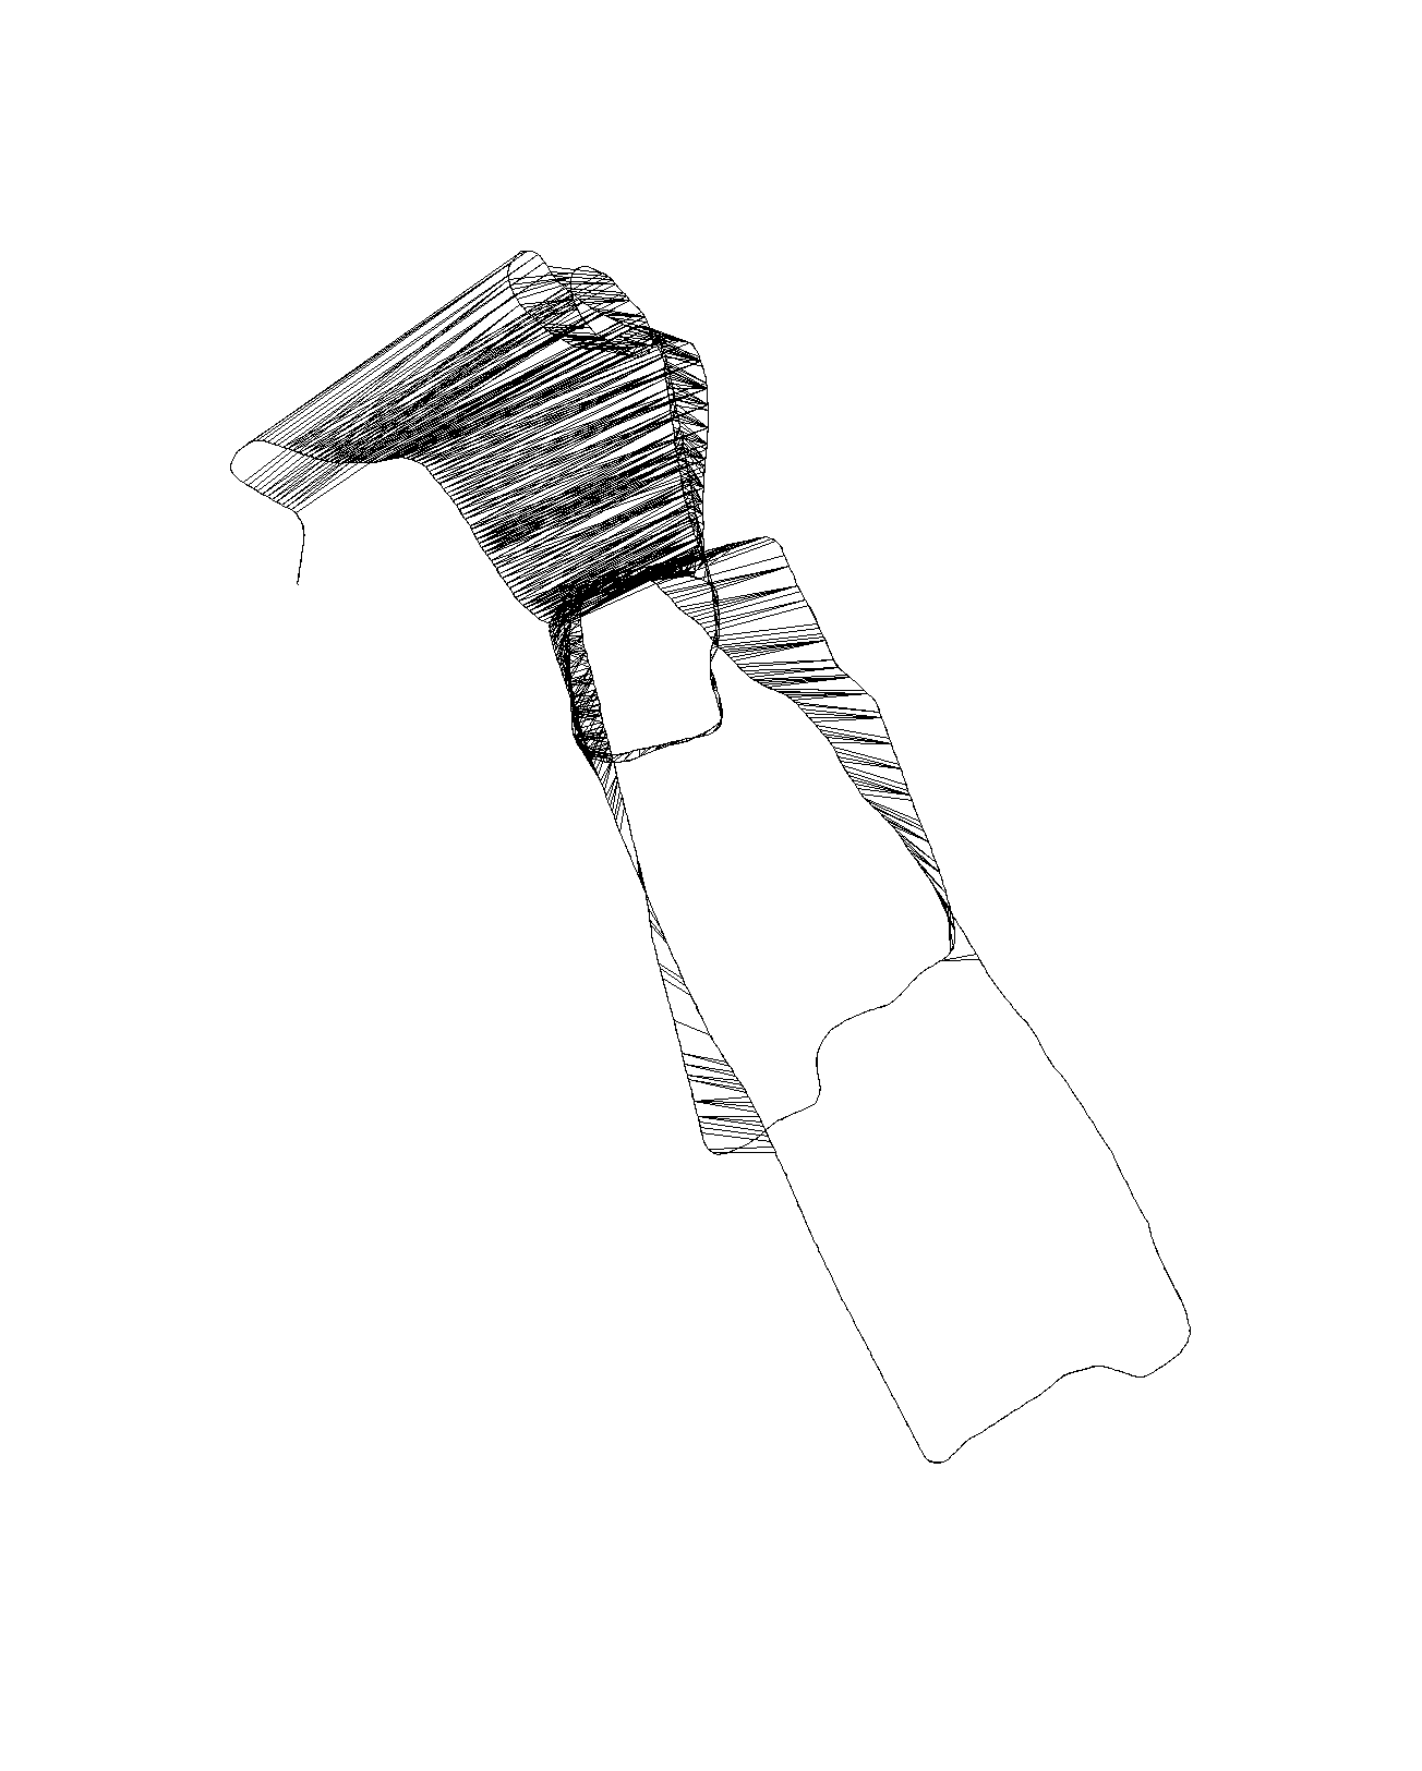
\includegraphics[width=0.7\textwidth]{images/pose_graph_constraints.png}}
    \only<4>{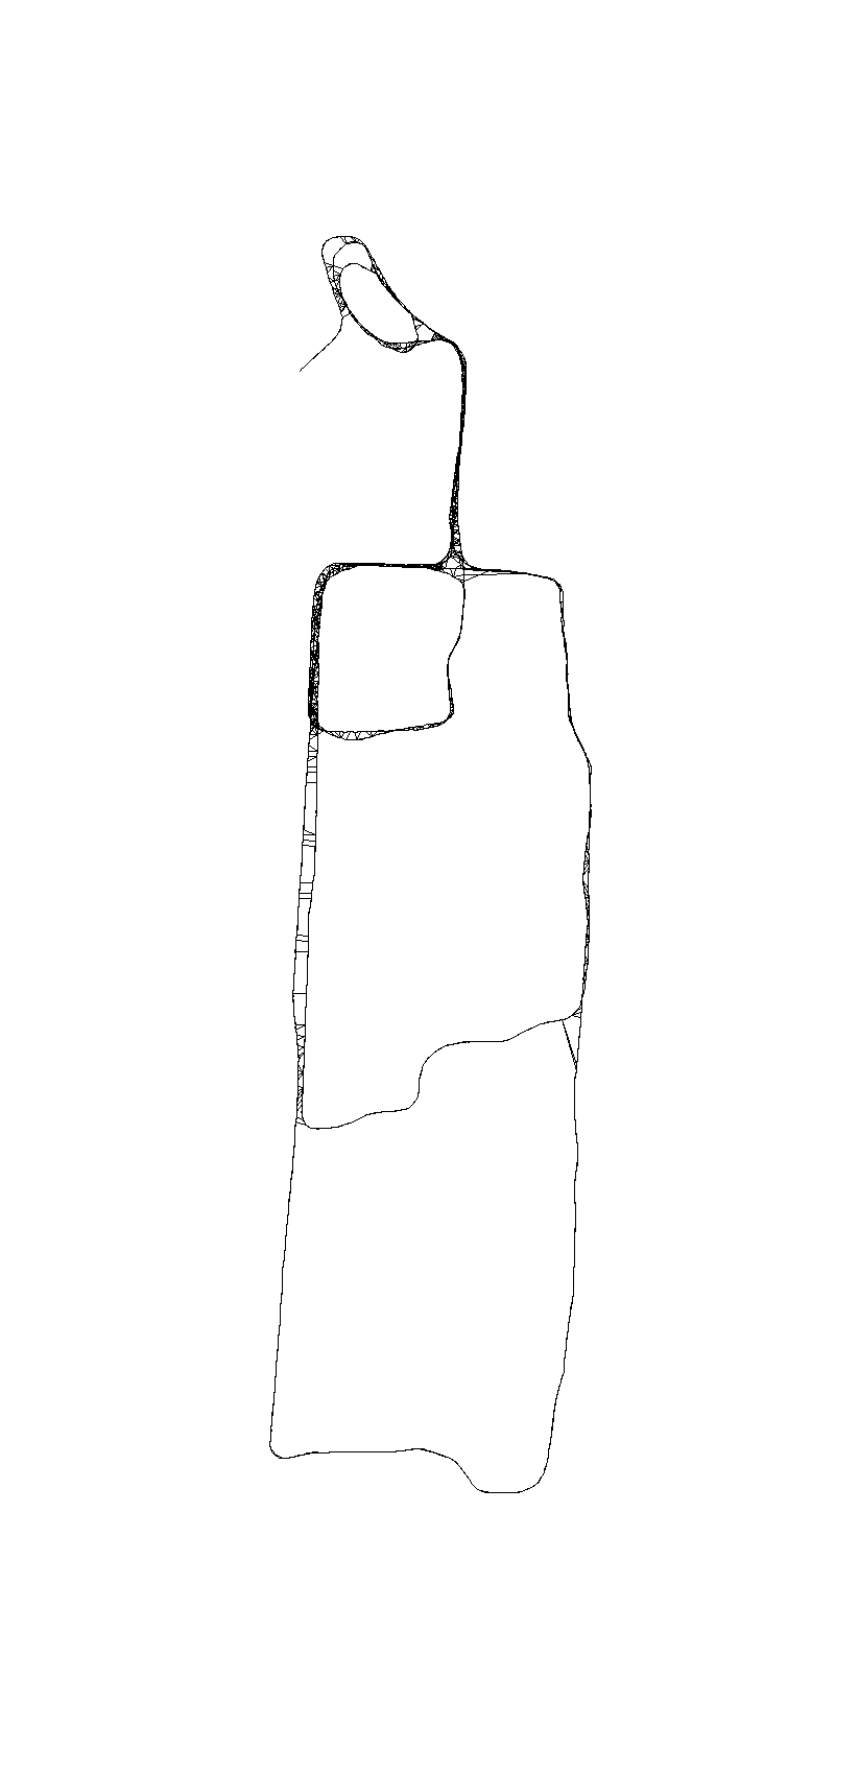
\includegraphics[width=0.5\textwidth]{images/pose_graph_optimized.png}}
    \only<5>{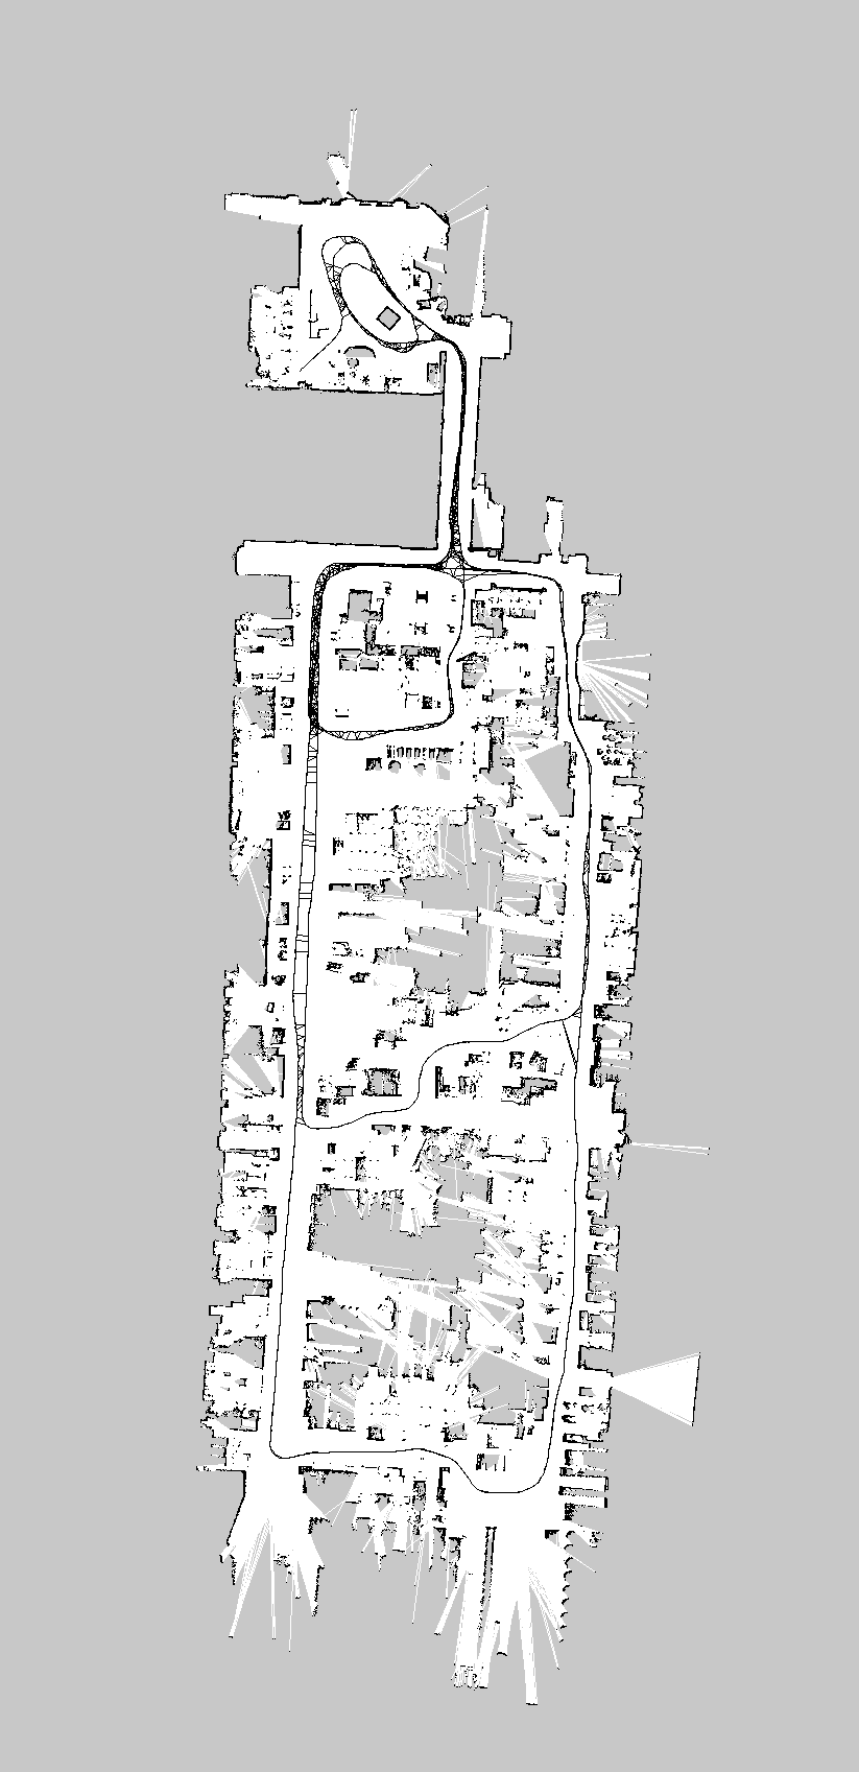
\includegraphics[width=0.5\textwidth]{images/pose_graph_optimized_with_map.png}}
    \end{column}
    \end{columns}
   
   \end{frame}
   
   \begin{frame}
    \frametitle{The graph in pose-graph}
    \note{Information taken from https://youtu.be/uHbRKvD8TWg}
   
    \begin{itemize}
    \item Consists of $n$ nodes $\stateBold = \stateBold_{1:n}$
    \item Each $\stateBold_{i}$ is a pose of the robot at time $t_{i}$
    \item A constraint/edge exists between node $\stateBold_{i}$ and $\stateBold_{j}$ if...
   \end{itemize}
   
   \begin{figure}[!h]
   \includegraphics[width=0.3\textwidth]{pose_graph_loop_example.pdf}
   \end{figure}
   
   \end{frame}
   
   \begin{frame}
   \frametitle{Create an edge if...}
   \note{Information taken from https://youtu.be/uHbRKvD8TWg}
   
   \begin{itemize}
   \item A constraint/edge exists between node $\stateBold_{i}$ and $\stateBold_{j}$ if the robot moves from $\stateBold_{i}$ to $\stateBold_{i+1}$
   \item The edges correspond to odometry
   \end{itemize}
   
   \begin{figure}[!h]
   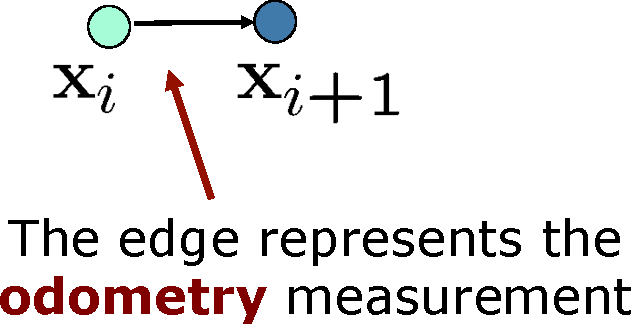
\includegraphics[width=0.44\textwidth]{pose_graph_odometry_edge.pdf}
   \end{figure}
   
   \end{frame}
   
   \begin{frame}
   \frametitle{Create an edge if...}
   \note{Information taken from https://youtu.be/uHbRKvD8TWg}
   
   \begin{itemize}
   \item<1-> A constraint/edge exists between node $\stateBold_{i}$ and $\stateBold_{j}$ if the robot observes the same part of the environment from $\stateBold_{i}$ and from $\stateBold_{j}$
   \item<2> We construct a {\bf virtual constraint} between the position of $\stateBold_{j}$ as seen from $\stateBold_{i}$
   \end{itemize}
   \only<1>{
   \begin{figure}
   \includegraphics[width=0.44\textwidth]{pose_graph_edge_lidar.pdf}
   \end{figure}
   }
   \only<2>{
   \begin{figure}
   \includegraphics[width=0.44\textwidth]{pose_graph_edge_lidar2.pdf}
   \end{figure}
   }
   
   \end{frame}
   
   \begin{frame}
   \frametitle{The edge information matrix}
   \note{Information taken from https://youtu.be/uHbRKvD8TWg}
   \begin{itemize}
   \item Observations are noisy
   \item The information matrix $\informationMatrix_{ij}$ for each edge encodes its uncertainty
   \item The larger the $\informationMatrix_{ij}$, the more important the edge is in the optimization.
   \end{itemize}
   
   \end{frame}
   
   \begin{frame}
    \frametitle{The edge information matrix}
    \note{Information taken from https://youtu.be/uHbRKvD8TWg}
    \begin{figure}[!h]
    \includegraphics[width=0.7\textwidth]{images/factor_graph_edge_example.pdf}
    \end{figure}
   
    Aim:
    \begin{equation*}
    \stateBold^{*} = \argmin_{\stateBold} \sum _{ij} \error^{\top}_{ij} \informationMatrix_{ij} \error_{ij}
    \end{equation*}
   
\end{frame}



\begin{frame}
    \frametitle{Least Squares in SLAM}
    \note{Information taken from https://youtu.be/uHbRKvD8TWg}
    We can minimize the error using least squares (\emph{Least Square})
    \begin{align*}
    \state^{*} &= \argmin_{\stateBold} \sum_{ij} \error^{\top}_{ij}(\stateBold_{i},\stateBold_{j}) \informationMatrix_{ij} \error_{ij}(\stateBold_{i},\stateBold_{j})\\
    &= \argmin_{\stateBold} \sum_{k} \error^{\top}_{k}(\stateBold) \informationMatrix_{k} \error_{k}(\stateBold)
    \end{align*}
    
    The {\bf state vector} is the Concatenation of the pose nodes $\stateBold = (\stateBold_{1}^{\top} \stateBold_{2}^{\top} \dots \stateBold_{n}^{\top})$. Each node is a pose (position or orientation).
    
    \vspace{2em}
    {\bf We need to define the error function...}
    \end{frame}
    
    \section{Least Squares}
    \begin{frame}
    \frametitle{Material para Least Squares}
    \note{Extraído de Curso de Cyrill Stachniss https://youtu.be/r2cyMQ5NB1o?si=WYODHSkWun3FL7jR}
    
    \TODO{Terminar slides de Least Squares}
    
    \begin{itemize}
        \item Cyrill Stachniss - Least Squares - An informal Introduction \url{https://youtu.be/r2cyMQ5NB1o?si=WYODHSkWun3FL7jR}
    \end{itemize}
\end{frame}


\begin{frame}
    \frametitle{Least Squares en General}
    \note{Extraído de Curso de Cyrill Stachniss https://youtu.be/r2cyMQ5NB1o?si=WYODHSkWun3FL7jR}
    
    Enfoque para calcular una solución para un sistema sobredeterminado

    \begin{itemize}
        \item Más ecuaciones que incógnitas
        \item Minimiza la suma de cuadrados de los errores en las ecuaciones
        \item Enfoque estándar para un gran conjunto de problemas
        \item Se utiliza para estimar el modelo de parámetros dado un conjunto de observaciones
    \end{itemize}
\end{frame}

\begin{frame}
    \frametitle{Nuestro Problema}
    \note{Extraído de Curso de Cyrill Stachniss https://youtu.be/r2cyMQ5NB1o?si=WYODHSkWun3FL7jR}
    
    Dado un sistema descripto por un conjunto de $n$ funciones de observación $\left\{f_{i}\left(\state\right)\right\}_{i=1:n}$

    \begin{itemize}
        \item $\stateBold$ es el vector de estado
        \item $\observationBold$ es una una medición del estado $\stateBold$
        \item $\prediction_{i} = f_{i}\left(\stateBold\right)$ es una función que mapea el estado $\stateBold$ a una medición predicha $\prediction_{i}$
        \item Dadas $n$ mediciones ruidosas $\observationBold_{1:n}$ acerca del estado $\stateBold$
        \item Objetivo: Estimar el estado $\stateBold$ que mejor explica las mediciones $\observationBold_{1:n}$
    \end{itemize}
\end{frame}

\begin{frame}
    \frametitle{Explicación Gráfica}
    \note{Extraído de Curso de Cyrill Stachniss https://youtu.be/r2cyMQ5NB1o?si=WYODHSkWun3FL7jR}
    
    \begin{center}
        \includegraphics[width=0.7\textwidth]{images/least_squares.pdf}
    \end{center}

\end{frame}

\begin{frame}
    \frametitle{Ejemplo}
    \note{Extraído de Curso de Cyrill Stachniss https://youtu.be/r2cyMQ5NB1o?si=WYODHSkWun3FL7jR}
    
    \begin{center}
        \includegraphics[width=0.7\textwidth]{images/least_squares.pdf}
    \end{center}
    
    \begin{itemize}
        \item $\stateBold$ posición de los puntos 3D
        \item $\observationBold_{i}$ coordenadas de los puntos 3D proyectados en las imágenes
        \item Estimar la posición 3D más probable de los puntos basado en las proyecciones en las imágenes (dada las poses de la cámara)
    \end{itemize}
\end{frame}

\begin{frame}
    \frametitle{Función de Error}
    \note{Extraído de Curso de Cyrill Stachniss https://youtu.be/r2cyMQ5NB1o?si=WYODHSkWun3FL7jR}
    
    \begin{itemize}
        \item El error $\error_{i}$ suele ser la diferencia entre la medición real y la predicción:
            \begin{equation*}
                \error_{i}\left( \stateBold \right) = \observationBold_{i} - f_{i}\left( \stateBold \right)
            \end{equation*}
        \item Supongamos que el error tiene una distribución normal con media cero
        \item Error Gaussiano con matriz de información $\informationMatrix_{i}$
        \item El error al cuadrado de una medición depende sólo del estado y es un escalar:
            \begin{equation*}
                \error_{i}\left( \stateBold \right) = \error_{i}\left( \stateBold \right)^{\top} \informationMatrix_{i} \error_{i}\left( \stateBold \right)
            \end{equation*}
    \end{itemize}
\end{frame}

\begin{frame}
    \frametitle{Objetivo: Encontrar el Mínimo}
    \note{Extraído de Curso de Cyrill Stachniss https://youtu.be/r2cyMQ5NB1o?si=WYODHSkWun3FL7jR}
    
    \begin{itemize}
        \item Encontrar el estado $\stateBold^{*}$ que minimiza el error dados todas las mediciones
        
        \begin{center}
            \includegraphics[width=0.7\textwidth]{images/find_minimum.pdf}
        \end{center}
    \end{itemize}

\end{frame}

\begin{frame}
    \frametitle{Objetivo: Encontrar el Mínimo}
    \note{Extraído de Curso de Cyrill Stachniss https://youtu.be/r2cyMQ5NB1o?si=WYODHSkWun3FL7jR}
    
    \begin{itemize}
        \item Encontrar el estado $\stateBold^{*}$ que minimiza el error dados todas las mediciones
        
        \begin{equation*}
            \stateBold^{*} = \argmin_{\stateBold} \sum_{i} \error_{i}\left( \stateBold \right)^{\top} \informationMatrix_{i} \error_{i}\left( \stateBold \right)
        \end{equation*}
        
        
        \item Una solución general es derivar la función de error global y encontrar sus nulos
        \item En general compleja y con solución no cerrada $\rightarrow$ Solución con Métodos numéricos
    \end{itemize}
    
\end{frame}


\begin{frame}
    \frametitle{Suposiciones}
    \note{Extraído de Curso de Cyrill Stachniss https://youtu.be/r2cyMQ5NB1o?si=WYODHSkWun3FL7jR}
    \begin{itemize}
        \item Hay una ``buena'' solución inicial disponible
        \item Las funciones de error son ``suaves'' en la vecindad del mínimo (con suerte global)
        \item Entonces, podemos resolver el problema con linearizaciones locales iterativas
    \end{itemize}

\end{frame}

\begin{frame}
    \frametitle{Resolvemos utilizando Linearizaciones locales iterativas}
    \note{Extraído de Curso de Cyrill Stachniss https://youtu.be/r2cyMQ5NB1o?si=WYODHSkWun3FL7jR}
    \begin{itemize}
        \item Linealizar los términos de error alrededor del solución actual/solución inicial
        \item Calcular la primera derivada de la función de error al cuadrado
        \item Setear en cero y resolver el sistema lineal
        \item Obtener el nuevo estado (que con suerte estará más cerca del mínimo)
        \item Iterar
    \end{itemize}
\end{frame}

\begin{frame}
    \frametitle{Linearizar la Función de Error}
    \note{Extraído de Curso de Cyrill Stachniss https://youtu.be/r2cyMQ5NB1o?si=WYODHSkWun3FL7jR}
    
    \begin{itemize}
        \item Podemos aproximar el error al rededor de una estimación inicial $\stateBold$ a través de una expansión de Taylor
    \end{itemize}
    
    \begin{equation*}
        \error_{i}(\stateBold + \vec{\Delta}\stateBold) \simeq  \underbrace{\error_{i}(\stateBold)}_{\error_{i}} + \jacobian_{i}\vec{\Delta}\stateBold \quad \text{con} \quad \jacobian_{i} = \dfrac{\partial\error_{i}(\stateBold)}{\partial\stateBold}
    \end{equation*}
    
\end{frame}

\begin{frame}
    \frametitle{Error Cuadrático}
    \note{Extraído de Curso de Cyrill Stachniss https://youtu.be/r2cyMQ5NB1o?si=WYODHSkWun3FL7jR}
    
    \begin{itemize}
        \item Con la linealización anterior, podemos fijar $\stateBold$ y llevar a cabo la minimización en los incrementos $\Delta\stateBold$
        \item Reemplazamos la expansión de Taylor en los términos de error al cuadrado:
        \only<1>{
            \begin{align*}
                e_{i}(\stateBold + \vec{\Delta}\stateBold) &= \dots
            \end{align*}
        }
        \only<2>{
            \begin{align*}
                e_{i}(\stateBold + \vec{\Delta}\stateBold) &= \error_{i}\left( \stateBold + \Delta \stateBold \right)^{\top} \informationMatrix_{i} \error_{i}\left( \stateBold  + \Delta \stateBold \right)
            \end{align*}
        }
        \only<3>{
            \begin{align*}
                e_{i}(\stateBold + \vec{\Delta}\stateBold) &= \error_{i}\left( \stateBold + \Delta \stateBold \right)^{\top} \informationMatrix_{i} \error_{i}\left( \stateBold  + \Delta \stateBold \right)\\
                &\simeq \left( \error_{i} + \jacobian_{i} \Delta \stateBold \right)^{\top} \informationMatrix_{i} \left( \error_{i} + \jacobian_{i} \Delta \stateBold \right)
            \end{align*}
        }
        \only<4>{
            \begin{align*}
                e_{i}(\stateBold + \vec{\Delta}\stateBold) &= \error_{i}\left( \stateBold + \Delta \stateBold \right)^{\top} \informationMatrix_{i} \error_{i}\left( \stateBold  + \Delta \stateBold \right)\\
                &\simeq \left( \error_{i} + \jacobian_{i} \Delta \stateBold \right)^{\top} \informationMatrix_{i} \left( \error_{i} + \jacobian_{i} \Delta \stateBold \right)\\
                &= \error_{i}^{\top} \informationMatrix_{i} \error_{i} + \error_{i}^{\top} \informationMatrix_{i} \jacobian_{i} \Delta \stateBold + \Delta \stateBold^{\top} \jacobian_{i}^{\top} \informationMatrix_{i} \error_{i} +  \Delta \stateBold^{\top} \jacobian_{i}^{\top} \informationMatrix_{i} \jacobian_{i} \Delta \stateBold
            \end{align*}
        }
    \end{itemize}
\end{frame}

\begin{frame}
    \frametitle{Error Cuadrático (cont.)}
    \note{Extraído de Curso de Cyrill Stachniss https://youtu.be/r2cyMQ5NB1o?si=WYODHSkWun3FL7jR}
    
    \begin{itemize}
        \item Todos los sumandos son escalares por lo que la transposición no tiene ningún efecto
        \item Agrupando términos similares obtenemos:
        \only<1>{
            \begin{align*}
                e_{i}(\stateBold + \vec{\Delta}\stateBold) &\simeq \error_{i}^{\top} \informationMatrix_{i} \error_{i} + \error_{i}^{\top} \informationMatrix_{i} \jacobian_{i} \Delta \stateBold + \Delta \stateBold^{\top} \jacobian_{i}^{\top} \informationMatrix_{i} \error_{i} +  \Delta \stateBold^{\top} \jacobian_{i}^{\top} \informationMatrix_{i} \jacobian_{i} \Delta \stateBold
            \end{align*}
        }
        \only<2>{
            \begin{align*}
                e_{i}(\stateBold + \vec{\Delta}\stateBold) &\simeq \error_{i}^{\top} \informationMatrix_{i} \error_{i} + \error_{i}^{\top} \informationMatrix_{i} \jacobian_{i} \Delta \stateBold + \Delta \stateBold^{\top} \jacobian_{i}^{\top} \informationMatrix_{i} \error_{i} +  \Delta \stateBold^{\top} \jacobian_{i}^{\top} \informationMatrix_{i} \jacobian_{i} \Delta \stateBold \\
                &= \underbrace{\error_{i}^{\top} \informationMatrix_{i} \error_{i}}_{c_{i}} + 2 \underbrace{\error_{i}^{\top} \informationMatrix_{i} \jacobian_{i}}_{\linearSystemb^{\top}_{i}} \Delta \stateBold + \Delta \stateBold^{\top} \underbrace{\jacobian_{i}^{\top} \informationMatrix_{i} \jacobian_{i}}_{\linearSystemH_{i}} \Delta \stateBold
            \end{align*}
        }
        \only<3>{
            \begin{align*}
                e_{i}(\stateBold + \vec{\Delta}\stateBold) &\simeq \error_{i}^{\top} \informationMatrix_{i} \error_{i} + \error_{i}^{\top} \informationMatrix_{i} \jacobian_{i} \Delta \stateBold + \Delta \stateBold^{\top} \jacobian_{i}^{\top} \informationMatrix_{i} \error_{i} +  \Delta \stateBold^{\top} \jacobian_{i}^{\top} \informationMatrix_{i} \jacobian_{i} \Delta \stateBold \\
                &= \underbrace{\error_{i}^{\top} \informationMatrix_{i} \error_{i}}_{c_{i}} + 2 \underbrace{\error_{i}^{\top} \informationMatrix_{i} \jacobian_{i}}_{\linearSystemb^{\top}_{i}} \Delta \stateBold + \Delta \stateBold^{\top} \underbrace{\jacobian_{i}^{\top} \informationMatrix_{i} \jacobian_{i}}_{\linearSystemH_{i}} \Delta \stateBold \\
                &= c_{i} + 2 \linearSystemb^{\top}_{i} \Delta \stateBold + \Delta \stateBold^{\top} \linearSystemH_{i} \Delta \stateBold
            \end{align*}
        }
    \end{itemize}
    
    
\end{frame}

\begin{frame}
    \frametitle{Error Global}
    \note{Extraído de Curso de Cyrill Stachniss https://youtu.be/r2cyMQ5NB1o?si=WYODHSkWun3FL7jR}
    
    \begin{itemize}
        \item El error global es la suma de términos de errores cuadrados correspondientes a las medidas individuales
        \item Forma una nueva expresión, que se aproxima al error global en la vecindad de la solución actual $\stateBold$
    \end{itemize}
    
    \begin{align*}
        F\left(\stateBold + \Delta \stateBold \right) &= \sum_{i} e_{i}(\stateBold + \vec{\Delta}\stateBold)\\
        F\left(\stateBold + \Delta \stateBold \right) &\simeq \sum_{i} \left( c_{i} + 2 \linearSystemb^{\top}_{i} \Delta \stateBold + \Delta \stateBold^{\top} \linearSystemH_{i} \Delta \stateBold \right) \\
        &= \sum_{i} c_{i} + 2 \left( \sum_{i} \linearSystemb^{\top}_{i} \right) \Delta \stateBold + \Delta \stateBold^{\top} \left( \sum_{i} \linearSystemH_{i} \right) \Delta \stateBold
    \end{align*}
    
    
\end{frame}

\begin{frame}
    \frametitle{Error Global (cont.)}
    \note{Extraído de Curso de Cyrill Stachniss https://youtu.be/r2cyMQ5NB1o?si=WYODHSkWun3FL7jR}
    
    \begin{align*}
        F\left(\stateBold + \Delta \stateBold \right) &\simeq \sum_{i} \left( c_{i} + 2 \linearSystemb^{\top}_{i} \Delta \stateBold + \Delta \stateBold^{\top} \linearSystemH_{i} \Delta \stateBold \right) \\
        &= \underbrace{\sum_{i} c_{i}}_{c} + 2 \underbrace{\left( \sum_{i} \linearSystemb^{\top}_{i} \right)}_{\linearSystemb^{\top}} \Delta \stateBold + \Delta \stateBold^{\top} \underbrace{\left( \sum_{i} \linearSystemH_{i} \right)}_{\linearSystemH} \Delta \stateBold \\
        &= c + 2 \linearSystemb^{\top} \Delta \stateBold + \Delta \stateBold^{\top} \linearSystemH \Delta \stateBold
    \end{align*}
    
    con
    
    \begin{align*}
        \linearSystemb^{\top} &= \sum_{i} \error_{i}^{\top} \informationMatrix_{i} \jacobian_{i} \\ 
        \linearSystemH &= \sum_{i}  \jacobian_{i}^{\top} \informationMatrix_{i} \jacobian_{i}
    \end{align*}
    
    
\end{frame}

\begin{frame}
    \frametitle{Forma Cuadrática}
    \note{Extraído de Curso de Cyrill Stachniss https://youtu.be/r2cyMQ5NB1o?si=WYODHSkWun3FL7jR}
    
    \begin{itemize}
        \item<1-> Podemos escribir los términos de error global como una forma cuadrática en $\Delta \stateBold$
        
        \begin{equation*}
            F\left(\stateBold + \Delta \stateBold \right) = c + 2 \linearSystemb^{\top} \Delta \stateBold + \Delta \stateBold^{\top} \linearSystemH \Delta \stateBold
        \end{equation*}
        
        \item<1> \alert{¿Cómo calcular el mínimo de una forma cuadrática?}
        \item<2-> Calcular la derivada de  $F\left(\stateBold + \Delta \stateBold \right)$ con respecto a $\Delta \stateBold$ (dado $\stateBold$)
        \item<2-> Derivamos e igualamos a 0
        \item<2-> resolvemos
    \end{itemize}

\end{frame}

\begin{frame}
    \frametitle{Derivando la forma cuadrática}
    \note{Extraído de Curso de Cyrill Stachniss https://youtu.be/r2cyMQ5NB1o?si=WYODHSkWun3FL7jR}
    
    \begin{itemize}
        \item Dada la forma cuadrática
        \begin{equation*}
            f(\stateBold) = \stateBold^{\top} \linearSystemH \stateBold + \linearSystemb^{\top} \stateBold
        \end{equation*}
        \item La primera derivada es
        \begin{equation*}
            \dfrac{\partial f}{\partial \stateBold} = \left( \linearSystemH + \linearSystemH^{\top} \right) \stateBold + \linearSystemb
        \end{equation*}
    \end{itemize}
    
    Ver: The Matrix Cookbook, sección 2.4.2
   
\end{frame}

\begin{frame}
    \frametitle{Forma Cuadrática}
    \note{Extraído de Curso de Cyrill Stachniss https://youtu.be/r2cyMQ5NB1o?si=WYODHSkWun3FL7jR}
    
    \begin{itemize}
        \item Podemos escribir los términos de error global de forma cuadrática en $\Delta \stateBold$
        \begin{equation*}
            F\left(\stateBold + \Delta \stateBold \right) = c + 2 \linearSystemb^{\top} \Delta \stateBold + \Delta \stateBold^{\top} \linearSystemH \Delta \stateBold
        \end{equation*}
        \item La derivada de $F\left(\stateBold + \Delta \stateBold \right)$
        \begin{equation*}
            \dfrac{\partial F\left(\stateBold + \Delta \stateBold \right)}{\partial \Delta \stateBold} \simeq 2 \linearSystemb + 2 \linearSystemH \Delta \stateBold
        \end{equation*}
    \end{itemize}
    
\end{frame}

\begin{frame}
    \frametitle{Minimizando la forma cuadrática}
    \note{Extraído de Curso de Cyrill Stachniss https://youtu.be/r2cyMQ5NB1o?si=WYODHSkWun3FL7jR}
    
    \begin{itemize}
        \item Derivada de $F\left(\stateBold + \Delta \stateBold \right)$
        \begin{equation*}
            \dfrac{\partial F\left(\stateBold + \Delta \stateBold \right)}{\partial \Delta \stateBold} \simeq 2 \linearSystemb + 2 \linearSystemH \Delta \stateBold
        \end{equation*}
        \item Igualando a 0
        \begin{equation*}
            0 = 2 \linearSystemb + 2 \linearSystemH \Delta \stateBold
        \end{equation*}
        \item Lo que lleva al sistema lineal
        \begin{equation*}
            \linearSystemH \Delta \stateBold = -\linearSystemb 
        \end{equation*}
        \item La solución para el incremento $\Delta \stateBold^{*}$ es
        \begin{equation*}
             \Delta \stateBold^{*} = - \inverse{\linearSystemH} \linearSystemb 
        \end{equation*}
    \end{itemize}
    
\end{frame}

\begin{frame}
    \frametitle{Solución con Gauss-Newton}
    \note{Extraído de Curso de Cyrill Stachniss https://youtu.be/r2cyMQ5NB1o?si=WYODHSkWun3FL7jR}
    
    Iterar los siguientes pasos:
    \begin{itemize}
        \item Lineanizar cerca de $\stateBold$ y computar para cada medición
        \begin{equation*}
            \error_{i}(\stateBold + \vec{\Delta}\stateBold) \simeq  \error_{i}(\stateBold) + \jacobian_{i}\vec{\Delta}\stateBold
        \end{equation*}
        \item Computar los términos del sistema lineal
        \begin{equation*}
            \linearSystemb^{\top} = \sum_{i} \error_{i}^{\top} \informationMatrix_{i} \jacobian_{i} \quad \quad \linearSystemH = \sum_{i} \jacobian_{i}^{\top} \informationMatrix_{i} \jacobian_{i}
        \end{equation*}
    \item Resolver el sistema lineal
    \begin{equation*}
        \Delta \stateBold^{*} = - \inverse{\linearSystemH} \linearSystemb 
    \end{equation*}
    \item Actualizar el estado
    \begin{equation*}
        \stateBold \leftarrow \stateBold + \Delta \stateBold^{*}
    \end{equation*} 
    \end{itemize}
    
\end{frame}

\begin{frame}
    \frametitle{Ejemplo: Calibración de Odometría}
    \note{Extraído de Curso de Cyrill Stachniss https://youtu.be/r2cyMQ5NB1o?si=WYODHSkWun3FL7jR}
    
    \begin{itemize}
        \item Mediciones de Odometría $\controlCommand_{i}$
        \item Eliminar el error sistemático a través de la calibración
        \item Suposición: disponemos del ground-truth de odometría $\controlCommand_{i}^{*}$
        \item Ground-truth dado por sistemas: Motion Capture (Vicon), Scan-Matching o SLAM
    \end{itemize}
    
\end{frame}

\begin{frame}
    \frametitle{Ejemplo: Calibración de Odometría}
    \note{Extraído de Curso de Cyrill Stachniss https://youtu.be/r2cyMQ5NB1o?si=WYODHSkWun3FL7jR}
    
    \begin{itemize}
        \item Hay una función que $f_{i}(\stateBold)$ que dado algunos parámetros de bias $\stateBold$, devuelve una odometría corregida (\emph{unbiased}) para la lectura ruidosa $\controlCommand_{i}^{\prime}$ 
        \begin{equation*}
            \controlCommand_{i}^{\prime} = f_{i}(\stateBold) =
            \begin{bmatrix}
                x_{11} & x_{12} & x_{13} \\
                x_{21} & x_{22} & x_{23} \\
                x_{31} & x_{32} & x_{33}
            \end{bmatrix}
            \controlCommand_{i}
        \end{equation*}
    \item Para obtener la función de corrección $f(\stateBold)$, necesitamos encontrar los parámetros $\stateBold$
    \end{itemize}
    
\end{frame}

\begin{frame}
    \frametitle{Calibración de Odoemtría (cont.)}
    \note{Extraído de Curso de Cyrill Stachniss https://youtu.be/r2cyMQ5NB1o?si=WYODHSkWun3FL7jR}
    \begin{itemize}

        \item El vector estado es 
        \begin{equation*}
            \stateBold =
            \begin{bmatrix}
                x_{11} & x_{12} & x_{13} & x_{21} & x_{22} & x_{23} & x_{31} & x_{32} & x_{33}
            \end{bmatrix}
        \end{equation*}
        \item La función error es
        \begin{equation*}
            \error_{i}(\stateBold) = \controlCommand_{i}^{*} - 
            \begin{bmatrix}
                x_{11} & x_{12} & x_{13} \\
                x_{21} & x_{22} & x_{23} \\
                x_{31} & x_{32} & x_{33}
            \end{bmatrix}
            \controlCommand_{i}
        \end{equation*}
        \item Su derivada es
        
    %    \begin{equation*}
    %        \jacobian_{i} = \dfrac{\partial \error_{i}(\stateBold)}{\partial \stateBold} = -
    %        \begin{bmatrix}
    %            u_{i,x} & u_{i,y} & u_{i,\theta} & 0 & 0 & 0 & 0 & 0 & 0 \\
    %            0 & 0 & 0 & u_{i,x} & u_{i,y} & u_{i,\theta} & 0 & 0 & 0 \\
    %            0 & 0 & 0 & 0 & 0 & 0 & u_{i,x} & u_{i,y} & u_{i,\theta}
    %        \end{bmatrix}
    %    \end{equation*}
    
        \begin{center}
            \includegraphics[width=0.8\columnwidth]{images/odometry_calibration_jacobian.pdf}
        \end{center}
        
        Que la primera derivada (Jacobiano) no dependa de $\stateBold$, es lo menos común, ya que significa que la función $\error$ es lineal!
        
        En este caso solo vamos a tener que hacer una sola iteración.

    \end{itemize}

    
\end{frame}

\begin{frame}
    \frametitle{Preguntas}
    \note{Extraído de Curso de Cyrill Stachniss https://youtu.be/r2cyMQ5NB1o?si=WYODHSkWun3FL7jR}
    
    \begin{itemize}
        \item<1-> ¿Cómo lucen los parámetros si la odometría es perfecta?
        \begin{itemize}
            \item<2-> La matriz debería ser la identidad. Entonces el error es 0, y por lo tanto, encontramos el mínimo.
        \end{itemize}
        \item<3-> ¿Cuantas mediciones son necesarias para encontrar la solución al problema de calibración?
        \begin{itemize}
            \item<4-> Tenemos que ver cuantas variables desconocidas tenemos y cuanta información nos provee cada observación. Tenemos 9 variables desconocidas. Cada observación nos da información de 3 variables (nos da 3 ecuaciones). Por lo tanto, vamos a necesitar al menos 3 observaciones.
        \end{itemize}
        \item<5-> $\linearSystemH$ es simétrica. ¿Por qué?
        \begin{itemize}
            \item<6-> La forma en que $\linearSystemH$ es simétrica porque  $\linearSystemH = \jacobian^{\top}\Omega\jacobian$. $\Omega$ es simétrica definida postiva y $\jacobian$ tambien, y por lo tanto el producto también.
        \end{itemize}
        \item<7-> ¿Cómo afecta la estructura de la función de medición a la estructura de $\linearSystemH$?
        \begin{itemize}
            \item<8-> $\linearSystemH$ es esparsa porque los jacobianos son esparsos. Los jacobianos son esparsos porque codifican cuanta información nos da una medición sobre todas las variables de estado. Por lo tanto, si nuestras mediciones solo relacionan algunas variables (como es el caso de SLAM), entonces la $\linearSystemH$ será esparsa.
        \end{itemize}
    \end{itemize}

\end{frame}

\begin{frame}
    \frametitle{¿Cómo Resolver de manera eficiente un Sistema Lineal?}
    \note{Extraído de Curso de Cyrill Stachniss https://youtu.be/r2cyMQ5NB1o?si=WYODHSkWun3FL7jR}
    \begin{itemize}
        \item Sistema Lineal $\linearSystemH \Delta \stateBold = -\linearSystemb$
        \item Podemos resolverlo utilizando inversión de matrices (en teoría)
        \item En la práctica:
        \begin{itemize}
            \item Factorización de Cholesky
            \item Descomposición QR
            \item Métodos iterativos como el método del Gradiente Conjugado (para sistemas grandes)
        \end{itemize}
        
    \end{itemize}
    
\end{frame}

\begin{frame}
    \frametitle{Descomposición de Cholesky para Resolver un Sistema Lineal}
    \note{Extraído de Curso de Cyrill Stachniss https://youtu.be/r2cyMQ5NB1o?si=WYODHSkWun3FL7jR}
    
    \begin{itemize}
        \item Sea la matriz $\vec{A}$ simétrica positiva definida
        \item El sistema a resolver es $\vec{A} \vec{x} = \vec{b}$
        \item Cholesky lleva a $\vec{A} = \vec{L} \vec{L}^{\top}$ con $\vec{L}$ matriz triangular inferior
        \item<2> Resolvemos primero
        \begin{equation*}
            \vec{L} \vec{y} = \vec{b}
        \end{equation*}
        \item<2> y luego,
        \begin{equation*}
            \vec{L}^{\top} \vec{x} = \vec{y}
        \end{equation*}
    
    \end{itemize}
    
\end{frame}

\begin{frame}
    \frametitle{Resumen de Gauss-Newton}
    \note{Extraído de Curso de Cyrill Stachniss https://youtu.be/r2cyMQ5NB1o?si=WYODHSkWun3FL7jR}
    
    Método para minimizar un error al cuadrado:
    \begin{itemize} 
        \item Comenzar con una solución inicial (\emph{initial guess})
        \item Linealizar las funciones de error individuales
        \item Esto lleva a una forma cuadrática
        \item Se obtiene un sistema lineal derivando e igualando a 0
        \item Resolver el sistema lineal conduce a una actualización del estado
        \item Iterar
    \end{itemize}
    
\end{frame}

\begin{frame}
    \frametitle{Least Squares vs. Probabilistic State Estimation}
    \note{Extraído de Curso de Cyrill Stachniss https://youtu.be/r2cyMQ5NB1o?si=WYODHSkWun3FL7jR}
    
    \begin{itemize}
        \item Hasta ahora, minimizamos una función de error
        \item ¿Cómo se relaciones esto con la estimación de estado en el sentido probabilístico?
    \end{itemize}
    
\end{frame}

\begin{frame}
    \frametitle{Comencemos con Estimación de estado}
    \note{Extraído de Curso de Cyrill Stachniss https://youtu.be/r2cyMQ5NB1o?si=WYODHSkWun3FL7jR}
    
    \begin{itemize}
        \item Regla de Bayes, suposiciones de independencia y Markov nos permiten reescribir
        \begin{equation*}
            p\left( \state_{0:t} | \observation_{1:t}, \controlCommand_{1:t} \right) = \eta p\left( \state_{0} \right) \prod_{t} \left[ p\left( \state_{t} | \state_{t-1}, \controlCommand_{t} \right) p\left( \observation_{t} | \state_{t} \right) \right]
        \end{equation*}
    \end{itemize}
    
    \note{p(x0) es un prior. Observar que en x0 no tenemos observaciones ni comandos de control}
    
\end{frame}

\begin{frame}
    \frametitle{Log Likelihood}
    \note{Extraído de Curso de Cyrill Stachniss https://youtu.be/r2cyMQ5NB1o?si=WYODHSkWun3FL7jR}
    
    \begin{itemize}
        \item Reescribiendo como el log likelihood, lleva a
        \begin{equation*}
            \log p\left( \state_{0:t} | \observation_{1:t}, \controlCommand_{1:t} \right) = \text{const.}  \log p\left( \state_{0} \right) + \sum_{t} \left[ \log p\left( \state_{t} | \state_{t-1}, \controlCommand_{t} \right) + \log p\left( \observation_{t} | \state_{t} \right) \right]
        \end{equation*}
    \end{itemize}
    
\end{frame}

\begin{frame}
    \frametitle{Suposición Gaussiana}
    \note{Extraído de Curso de Cyrill Stachniss https://youtu.be/r2cyMQ5NB1o?si=WYODHSkWun3FL7jR}
    
    \begin{itemize}
        \item Suponiendo distribución Gaussiana
        \begin{equation*}
            \log p\left( \state_{0:t} | \observation_{1:t}, \controlCommand_{1:t} \right) = \text{const.}  \log \underbrace{p\left( \state_{0} \right)}_{\mathcal{N}} + \sum_{t} \left[ \log \underbrace{p\left( \state_{t} | \state_{t-1}, \controlCommand_{t} \right)}_{\mathcal{N}} + \log \underbrace{p\left( \observation_{t} | \state_{t} \right)}_{\mathcal{N}} \right]
        \end{equation*}
    \end{itemize}
    
\end{frame}

\begin{frame}
    \frametitle{Log de una Gaussiana}
    \note{Extraído de Curso de Cyrill Stachniss https://youtu.be/r2cyMQ5NB1o?si=WYODHSkWun3FL7jR}

    
    \begin{itemize}
        \item La función de distribución de la distribución normal está definida como
        \begin{equation*}
            p(x)=\det(2\pi\covariance)^{\frac{1}{2}} \exp\left(-\dfrac{1}{2} (x - \mu )^{\top} \inverse{\covariance} (x - \mu )  \right)
        \end{equation*}
        
        \item Log likelihood de una Gaussiana
        \begin{equation*}
            \log \mathcal{N}(x, \mu, \Sigma) =  \text{const.} - \dfrac{1}{2} (x - \mu)^{\top} \inverse{\Sigma} (x - \mu)
        \end{equation*}
    \end{itemize}
    
\end{frame}

\begin{frame}
    \frametitle{Función de Error como Exponente}
    \note{Extraído de Curso de Cyrill Stachniss https://youtu.be/r2cyMQ5NB1o?si=WYODHSkWun3FL7jR}
    
    \begin{itemize}
        \item Log likelihood de una Gaussiana
        \begin{equation*}
            \log \mathcal{N}(x, \mu, \Sigma) =  \text{const.} - \dfrac{1}{2} \underbrace{\underbrace{(x - \mu)^{\top}}_{\error^{\top}(x)} \underbrace{\inverse{\Sigma}}_{\informationMatrix} \underbrace{(x - \mu)}_{\error(x)}}_{e(x)}
        \end{equation*}
        \item está a una constante de equivalencia de las funciones de error usadas antes
    \end{itemize}
    
\end{frame}

\begin{frame}
    \frametitle{Log Likelihood con Términos de Error}
    \note{Extraído de Curso de Cyrill Stachniss https://youtu.be/r2cyMQ5NB1o?si=WYODHSkWun3FL7jR}
    
    \begin{itemize}
        \item Suponiendo distribución Gaussiana
        \begin{equation*}
            \log p\left( \state_{0:t} | \observation_{1:t}, \controlCommand_{1:t} \right) = \text{const.} - \dfrac{1}{2} e_{p}(\state) -  \dfrac{1}{2} \sum_{t} \left[ e_{\controlCommand_{t}}(\state) + e_{\observation_{t}}(\state)\right]
        \end{equation*}
    \end{itemize}
    
\end{frame}

\begin{frame}
    \frametitle{Maximizing el Log Likelihood}
    \note{Extraído de Curso de Cyrill Stachniss https://youtu.be/r2cyMQ5NB1o?si=WYODHSkWun3FL7jR}
    
    \begin{itemize}
        \item Suponiendo distribución Gaussiana
        \begin{equation*}
            \log p\left( \state_{0:t} | \observation_{1:t}, \controlCommand_{1:t} \right) = \text{const.} - \dfrac{1}{2} e_{p}(\state) -  \dfrac{1}{2} \sum_{t} \left[ e_{\controlCommand_{t}}(\state) + e_{\observation_{t}}(\state)\right]
        \end{equation*}
        \item Maximizando el log likelihood lleva a 
        \begin{equation*}
            \argmax \log p\left( \state_{0:t} | \observation_{1:t}, \controlCommand_{1:t} \right) = \argmin e_{p}(\state) + \sum_{t} \left[ e_{\controlCommand_{t}}(\state) + e_{\observation_{t}}(\state)\right]
        \end{equation*}
    \end{itemize}
    
    
\end{frame}

\begin{frame}
    \frametitle{Minimizar el error cuadrático es equivalente a Maximizar el Log Likelihood de Distribuciones Gaussianas Independientes}
    \note{Extraído de Curso de Cyrill Stachniss https://youtu.be/r2cyMQ5NB1o?si=WYODHSkWun3FL7jR}
    \begin{itemize}
        \item Con términos de error individuales para los controles, mediciones y un prior:
        \begin{equation*}
            \argmax \log p\left( \state_{0:t} | \observation_{1:t}, \controlCommand_{1:t} \right) = \argmin e_{p}(\state) + \sum_{t} \left[ e_{\controlCommand_{t}}(\state) + e_{\observation_{t}}(\state)\right]
        \end{equation*}
    \end{itemize}
    
\end{frame}

\begin{frame}
    \frametitle{Resumen}
    \note{Extraído de Curso de Cyrill Stachniss https://youtu.be/r2cyMQ5NB1o?si=WYODHSkWun3FL7jR}
    
    \begin{itemize}
        \item Técnica para minimizar funciones de error cuadráticas
        \item Gauss-Newton es un enfoque iterativo para problemas no lineales
        \item Utiliza linearización (¡aproximación!)
        \item Equivalente a maximizar el log likelihood de Gaussianas independientes
        \item Método popular en muchas disciplinas.
    \end{itemize}

    
\end{frame}

\begin{frame}
    \frametitle{Bibliografía de Gauss-Newton}
    \note{Extraído de Curso de Cyrill Stachniss https://youtu.be/r2cyMQ5NB1o?si=WYODHSkWun3FL7jR}
    \begin{itemize}
        \item Capítulo 11.4 de \cite{thrun2005probabilistic}
    \end{itemize}
\end{frame}
    
    \begin{frame}
    \frametitle{Error Function}
    \note{Information taken from https://youtu.be/uHbRKvD8TWg}
    
    \begin{itemize}
    \item Error Function for a Single Constraint
    \begin{figure}
    \includegraphics[width=0.44\textwidth]{pose_graph_error_function.pdf}
    \end{figure}
    \footnotetext{$t2v(.)$ maps transformations to vectors}
    
    \item Error as a Function of a Full State Vector
    
    \begin{equation*}
    \error_{ij}(\state) = t2v(\inverse{\observationBold}_{ij}(\inverse{\stateBold}_{i}\stateBold_{j}))
    \end{equation*}
    
    \item The error takes the value 0 when
    
    \begin{equation*}
    \observationBold_{ij} = (\inverse{\stateBold}_{i}\stateBold_{j})
    \end{equation*}
    
    \end{itemize}
    \end{frame}
    
    \begin{frame}
    \frametitle{Linearizing the error function}
    \note{Information taken from https://youtu.be/uHbRKvD8TWg}
    
    \begin{itemize}
    \item We can approximate the error around an initial estimate $\stateBold$ through a Taylor expansion
    \end{itemize}
    
    \begin{equation*}
    \error_{ij}(\stateBold + \vec{\Delta}\stateBold) \simeq \error_{ij}(\stateBold) + \jacobian_{ij}\vec{\Delta}\stateBold \quad \text{con} \quad \jacobian_{ij} = \dfrac{\partial\error_{ij}(\stateBold)}{\partial\stateBold}
    \end{equation*}
    
    \end{frame}
    
    \begin{frame}
    \frametitle{Derivative of the error function}
    \note{Information taken from https://youtu.be/uHbRKvD8TWg}
    \begin{itemize}
    \item<1-> Question: Does an error term $\error_{ij}(\stateBold)$ depend on all state variables?
    
    \only<2->{No, it only depends on $\stateBold_{i}$ and $\stateBold_{j}$}
    
    \item<3-> Question: Are there any consequences for the structure of the Jacobian?
    
    \only<4->{
     Yes, it will be different from zero only in the rows corresponding to $\stateBold_{i}$ and $\stateBold_{j}$
    
     \begin{align*}
     \dfrac{\partial\error_{ij}(\stateBold)}{\partial\stateBold} &=
     \begin{bmatrix}
     0 & \dots & \dfrac{\partial\error_{ij}(\stateBold_{i})}{\partial\stateBold_{i}} & \dots & 0 & \dots & \dfrac{\partial\error_{ij}(\stateBold_{j})}{\partial\stateBold_{j}} & \dots & 0
     \end{bmatrix} \\
     \jacobian_{ij} &=
     \begin{bmatrix}
     0 & \dots & \vec{A}_{ij} & \dots & 0 & \dots & \vec{B}_{ij} & \dots & 0
     \end{bmatrix}
     \end{align*}
     }
    
    
     \end{itemize}
    
    \end{frame}
    
    
    \begin{frame}
     \frametitle{Jacobians and the sparse problem}
     \note{Information taken from https://youtu.be/uHbRKvD8TWg}
    
     \begin{itemize}
     \item The error $\error_{ij}(\stateBold)$ depends only on the parameter blocks $\stateBold_{i}$ and $\stateBold_{j}$
    
     \begin{equation*}
     \error_{ij}(\stateBold) =\error_{ij}(\stateBold_{i} ,\stateBold_{j})
     \end{equation*}
    
     \item The Jacobian will be zero everywhere except in the columns $\stateBold_{i}$ and $\stateBold_{j}$
    
     \begin{equation*}
     \jacobian_{ij} =
     \begin{bmatrix}
     0 & \dots & 0 & \dfrac{\partial\error_{ij}(\stateBold_{i})}{\partial\stateBold_{i}} & 0 & \dots & 0 & \dfrac{\partial\error_{ij}(\stateBold_{j})}{\partial\stateBold_{j}} & 0 & \dots & 0
     \end{bmatrix}
     \end{equation*}
    
     \end{itemize}
    
     {\bf This allows us to solve SLAM efficiently!}
    
\end{frame}


\begin{frame}
    \frametitle{Consequence of this being a sparse problem}
    \note{Information taken from https://youtu.be/uHbRKvD8TWg}
    
    \begin{itemize}
    \item We need to compute the coefficient vector.
    \begin{align*}
    \linearSystemb^{\top} &= \sum_{ij} \linearSystemb_{ij}^{\top} = \sum_{ij} \error_{ij}^{\top}\Omega_{ij}\jacobian_{ij}\\
    \linearSystemH &= \sum_{ij} \linearSystemH_{ij} = \sum_{ij} \jacobian_{ij}^{\top}\Omega_{ij}\jacobian_{ij}
    \end{align*}
    \item The sparse structure of $\jacobian_{ij}$ will result in a sparse structure of $\linearSystemH$
    \item This structure reflects the graph's adjacency matrix.
    \end{itemize}
    
    \end{frame}
    
    \begin{frame}
    \frametitle{Illustration of the structure}
    \note{Information taken from https://youtu.be/uHbRKvD8TWg}
    
    \begin{figure}[!h]
    \includegraphics[width=0.9\textwidth]{linear_system_sparsity.pdf}
    \end{figure}
    
    \end{frame}
    
    \begin{frame}
    \frametitle{Consequence of it being a sparse problem}
    \note{Information taken from https://youtu.be/uHbRKvD8TWg}
    
    \begin{figure}[!h]
    \includegraphics[width=0.9\textwidth]{linear_system_sparsity2.pdf} 
    \end{figure}
    
    \end{frame}
    
    \begin{frame}
     \frametitle{Consequence of it being a dispersed problem}
     \note{Information taken from https://youtu.be/uHbRKvD8TWg}
    
     \begin{itemize}
     \item An edge contributes to the linear system through $\linearSystemb_{ij}$ and $\linearSystemH_{ij}$
     \item The coefficient vector is
    
     \begin{align*}
     \linearSystemb_{ij}^{\top} &= \error_{ij}^{\top}\informationMatrix_{ij}\jacobian_{ij}\\
     &= \error_{ij}^{\top}\informationMatrix_{ij}
     \begin{bmatrix}
     0 & \dots & \vec{A}_{ij} & \dots & \vec{B}_{ij} & \dots & 0
    \end{bmatrix}\\
    &=
    \begin{bmatrix}
    0 & \dots & \error_{ij}^{\top}\informationMatrix_{ij}\vec{A}_{ij} & \dots & \error_{ij}^{\top}\informationMatrix_{ij}\vec{B}_{ij} & \dots & 0
    \end{bmatrix}
    \end{align*}
    \item It is nonzero only at the corresponding indices of $\stateBold_{i}$ and $\stateBold_{j}$
    \end{itemize}
    
    \end{frame}
    
    \begin{frame}
    \frametitle{Consequence of it being a sparse problem}
    \note{Information taken from https://youtu.be/uHbRKvD8TWg}
    \small
    \begin{itemize}
    \item The coefficient matrix of an edge is
     \begin{align*}
     \linearSystemH_{ij}^{\top} &= \jacobian_{ij}^{\top}\informationMatrix_{ij}\jacobian_{ij}\\
     &=
     \begin{bmatrix}
     \vdots \\
     \vec{A}_{ij}^{\top}\\
     \vdots \\
     \vec{B}_{ij}^{\top}\\
     \vdots
     \end{bmatrix} \informationMatrix_{ij}
     \begin{bmatrix}
     \cdots & \vec{A}_{ij} & \cdots & \vec{B}_{ij} & \cdots
     \end{bmatrix}\\
     &=
     \begin{bmatrix}
     0 & \cdots & 0 & \cdots & 0 \\
     \vdots & \vec{A}_{ij}^{\top}\informationMatrix_{ij}\vec{A}_{ij} & \vdots & \vec{A}_{ij}^{\top}\informationMatrix_{ij}\vec{B}_{ij} & \vdots\\
     0 & \cdots & 0 & \cdots & 0 \\
     \vdots & \vec{B}_{ij}^{\top}\informationMatrix_{ij}\vec{A}_{ij} & \vdots & \vec{B}_{ij}^{\top}\informationMatrix_{ij}\vec{B}_{ij} & \vdots\\
     0 & \cdots & 0 & \cdots & 0
     \end{bmatrix}
     \end{align*}
     \item Is non-zero in related blocks with $i,j$
    \end{itemize}
    
    \end{frame}
    
    \begin{frame}
    \frametitle{Summary of the sparse problem}
    \note{Information taken from https://youtu.be/uHbRKvD8TWg}
    
    \begin{itemize}
    \item An edge ij only contributes to
    \begin{itemize}
    \item the i-th and j-th blocks of $\linearSystemb_{ij}$
    \item the blocks $ii$, $jj$, $ij$, and $ji$ of $\linearSystemH_{ij}$
    \end{itemize}
    \item The resulting system is sparse.
    \item The system can be computed by summing the contributions of each edge.
    \item Different \emph{solvers} can be used.
    \begin{itemize}
    \item Sparse Cholesky decomposition.
    \item Conjugate gradient. \item many more...
     \end{itemize}
    
     \end{itemize}
    
    
\end{frame}

\begin{frame}
    \frametitle{The Linear System}
    \note{Information taken from https://youtu.be/uHbRKvD8TWg}
   
    \begin{itemize}
    \item Vector of state increments
    \begin{equation*}
    \Delta\stateBold^{\top} =
    \begin{bmatrix}
    \Delta\stateBold_{1}^{\top} & \Delta\stateBold_{2}^{\top} & \cdots & \Delta\stateBold_{n}^{\top}
    \end{bmatrix}
    \end{equation*}
    \item Coefficient vector
    \begin{equation*}
    \linearSystemb^{\top} =
    \begin{bmatrix}
    \overline{\linearSystemb}_{1}^{\top} & \overline{\linearSystemb}_{2}^{\top} & \cdots & \overline{\linearSystemb}_{n}^{\top}
    \end{bmatrix}
    \end{equation*}
    \item Matrix of normal equations
    \begin{equation*}
    \linearSystemH =
    \begin{bmatrix}
    \overline{\linearSystemH}_{11} & \overline{\linearSystemH}_{12} & \cdots & \overline{\linearSystemH}_{1n}\\
    \overline{\linearSystemH}_{21} & \overline{\linearSystemH}_{22} & \cdots & \overline{\linearSystemH}_{2n}\\
    \vdots & \vdots & \ddots & \vdots\\
    \overline{\linearSystemH}_{n1} & \overline{\linearSystemH}_{n2} & \cdots & \overline{\linearSystemH}_{nn}\\
   \end{bmatrix}
   \end{equation*}
   \end{itemize}
   
   \end{frame}
   
   \begin{frame}
   \frametitle{Construction of the linear system}
   \note{Information taken from https://youtu.be/uHbRKvD8TWg}
   For each constraint:
   \begin{itemize}
   \item Compute the error $\error_{ij} = t2v(\inverse{\observationBold}_{ij}(\inverse{\stateBold}_{i}\stateBold_{j}))$
   \item Compute the blocks of the Jacobians:
   \begin{equation*}
   \vec{A}_{ij} = \dfrac{\partial\error _{ij}(\stateBold _{i}, \stateBold _{j})}{\partial\stateBold _{i}} \quad \quad \vec{B}_{ij} = \dfrac{\partial\error _{ij}(\stateBold _{i}, \stateBold _{j})}{\partial\stateBold _{j}}
    \end{equation*}
    \item Update the coefficient vector:
    \begin{equation*}
    \overline{\linearSystemb}_{i}^{\top} += \error_{ij}^{\top}\informationMatrix_{ij}\vec{A}_{ij} \quad \quad \overline{\linearSystemb}_{j}^{\top} += \error_{ij}^{\top}\informationMatrix_{ij}\vec{B}_{ij}
    \end{equation*}
   
    \item Update the coefficient vector:
    \begin{align*}
    \overline{\linearSystemH}_{ij}^{\top} &+= \vec{A}_{ij}^{\top}\informationMatrix_{ij}\vec{A}_{ij} \quad \quad \overline{\linearSystemH}_{ij}^{\top} += \vec{A}_{ij}^{\top}\informationMatrix_{ij}\vec{B}_{ij} \\
    \overline{\linearSystemH}_{ij}^{\top} &+= \vec{B}_{ij}^{\top}\informationMatrix_{ij}\vec{A}_{ij} \quad \quad \overline{\linearSystemH}_{ij}^{\top} += \vec{B}_{ij}^{\top}\informationMatrix_{ij}\vec{B}_{ij}
    \end{align*}
    \end{itemize}
   
   \end{frame}
   
   \begin{frame}
    \frametitle{Algorithm}
    \note{Information taken from https://youtu.be/uHbRKvD8TWg}
   
    \begin{algorithmic}[1]
    \Procedure{optimize}{$\stateBold$}
    \While (!converged)
    \State $(\linearSystemH,\linearSystemb) = buildLinearSystem(\stateBold)$
    \State $\vec{\Delta}\stateBold = solveSparse(\linearSystemH\vec{\Delta}\stateBold = -\linearSystemb)$
    \State $\stateBold = \stateBold + \vec{\Delta}\stateBold$
    \EndWhile
   
    \State \Return $\stateBold$
    \EndProcedure
    \end{algorithmic}
   
   \end{frame}
   
   
   \begin{frame}
    \frametitle{1D Trivial Example}
    \note{Information taken from https://youtu.be/uHbRKvD8TWg}
   
    Two nodes and one observation
   
    \begin{figure}[!h]
    \includegraphics[width=0.2\textwidth]{pose_graph_1d_example.pdf}
    \end{figure}
   
    \small
   
    \begin{align*}
    \stateBold &=
    \begin{bmatrix}
    \stateBold_{1} & \stateBold_{2}
    \end{bmatrix}^{\top}
    =
    \begin{bmatrix}
    0 & 0
    \end{bmatrix}\\
    \observationBold_{12} &= 1\\
    \informationMatrix_{12} &= 2\\
    \error_{12} &= \observationBold_{12} - (\stateBold_{2} - \stateBold_{1}) = 1 - (0 - 0) = 1\\
    \jacobian_{12} &=
    \begin{bmatrix}
    1 & -1
    \end{bmatrix}\\
    \linearSystemb_{12}^{\top} &= \error_{12}^{\top} \informationMatrix_{12} \jacobian_{12} =
    \begin{bmatrix}
    2 & -2
    \end{bmatrix}\\
    \linearSystemH_{12} &= \jacobian_{12}^{\top} \informationMatrix_{12} \jacobian_{12} =
    \begin{bmatrix}
    2 & -2\\
    -2 & 2
    \end{bmatrix}\\
    \vec{\Delta}\stateBold &= -\inverse{\linearSystemH}_{12} \linearSystemb_{12}\\
    \end{align*}
   
    \begin{center}
    \alert{Problem:} $\det(\linearSystemH) = 0$, therefore we cannot invert $\linearSystemH$
    \end{center}
\end{frame}

\begin{frame}
    \frametitle{What's wrong?}
    \note{Information taken from https://youtu.be/uHbRKvD8TWg}
    
    \begin{itemize}
    \item The constraint specifies a relative constraint between both nodes.
    \item Any pose of the nodes will be correct if the relative constraint between them is met. This problem is known as {\bf Gauge Freedom}
    \item To solve it, we have to {\bf fix} a node. By fixing a node, we are adding a {\bf Prior}!
    \end{itemize}
    
    \begin{align*}
    \linearSystemH &=
    \begin{bmatrix}
    2 & -2\\
    -2 & 2
    \end{bmatrix}
    +
    \begin{bmatrix}
    1 & 0\\
    0 & 0
    \end{bmatrix} \leftarrow \text{restriction that puts } \vec{\Delta}\stateBold_{1} = 0\\
    \vec{\Delta}\stateBold &= -\inverse{\linearSystemH}_{12} \linearSystemb_{12}\\
    \vec{\Delta}\stateBold &=
    \begin{bmatrix}
    0 & 1
    \end{bmatrix}^{\top}
    \end{align*}
    
    With this we make the update of node $\stateBold_{1}$ to be 0 and the update of $\stateBold_{2}$ is updated with 1.
    \end{frame}
    
    \begin{frame}
    \frametitle{Role of the Prior}
    \note{Information taken from https://youtu.be/uHbRKvD8TWg}
    
    \begin{itemize}
    \item We saw that the information matrix $\linearSystemH$ is not of full rank, and therefore not invertible.
    \item A global reference frame has not been fixed.
    \item Fixing a global reference frame is strongly related to the prior $p(\stateBold_{0})$.
    \item A Gaussian estimate of $\stateBold_{0}$ results in adding a constraint.
    \item Example: The first pose must be fixed at the origin.
    \begin{equation*}
    \error(\stateBold_{0}) = t2v(\stateBold_{0})
    \end{equation*}
    That is, To minimize, we want the error term $\error(\stateBold_{0})$ to be as small as possible. This happens when $\stateBold_{0}$ tends to 0.
    \end{itemize}
    
    \end{frame}
    
    \begin{frame}
    \frametitle{Fixing a subset of variables}
    \note{Information taken from https://youtu.be/uHbRKvD8TWg}
    
    \begin{itemize}
    \item We assume that the value of certain variables during the optimization is known a priori.
    \item We want to optimize all the other variables but keep them fixed.
    \item We can do as we did with the previous prior, but the problem is that it is only a {\bf soft constraint} and not really a fix. Another constraint may move this node, and therefore we cannot guarantee that it has a fixed value.
    \item \textbf{To effectively make a variable fixed, we must make it non-optimizable, and therefore we must remove it from the linear system}. Removing it from the linear system means it is not updated, and all other variables are constrained by it. This is done by constructing the entire linear system and then simply deleting the row and column corresponding to the variable. Finally, the linear system is solved. \item Column and row suppression works as a {\bf conditioning}, that is, it is a condition that says, "Since a node takes a value, the others are affected in this way."
    
    \end{itemize}
    
    \end{frame}
    
    \begin{frame}
    \frametitle{We can suppress the columns and rows of the corresponding variables}
    \note{Information taken from https://youtu.be/uHbRKvD8TWg}
    
    \begin{itemize}
    \item The reason we can do this stems from {\bf conditioning on Gaussian distributions}.
    \item {\bf Conditioning in the information space} means that we can remove a portion of the information matrix, and this corresponds to a conditioning operation on the Gaussian distribution.
    \item The $\linearSystemH$ is an information matrix of our entire problem with all the constraints put together. Therefore, by removing a row and a column, we are conditioning the system by making them fixed and non-updatable, and by restricting all other variables.
    \end{itemize}
    
    \footnotetext{More info in the paper: Exactly sparse delayed-state filters for view-based SLAM. Eustice, Ryan M., Singh, Hanumant, Leonard, John J.}
    
\end{frame}

\begin{frame}
    \frametitle{Uncertainty}
    \note{Information taken from https://youtu.be/uHbRKvD8TWg}
    
    \begin{itemize}
    \item $\linearSystemH$ represents the information matrix given the linearization point.
    \item The inverse of $\linearSystemH$ is the (dense) covariance matrix. Computing the inverse is computationally very expensive. However, we can compute parts of the covariance matrix.
    \item The blocks on the diagonal of the covariance matrix represent the uncertainties of the corresponding variables.
    \end{itemize}
    \end{frame}
    
    \begin{frame}
    \frametitle{Relative Uncertainty}
    \note{Information taken from https://youtu.be/uHbRKvD8TWg}
    \begin{itemize}
    \item Determine the relative uncertainty between $\stateBold_{i}$ and $\stateBold_{j}$.
    
    \begin{itemize}
    \item This is especially useful for cycle detection, as we can compute the uncertainty of the current pose relative to a previous pose. This allows us to determine whether a cycle is possible between poses or not (if the previous pose is within the covariance, then we detect a cycle).
    \end{itemize}
    
    \item To determine the relative uncertainty between $\stateBold_{i}$ and $\stateBold_{j}$ we will:
    \begin{itemize}
    \item Build the complete matrix $\linearSystemH$
    \item Delete the rows and columns of $\stateBold_{i}$ (equivalent to not optimizing/fixing the variable)
    \item Compute the $j,j$ block of the inverse
    \item This block contains the covariance matrix of $\stateBold_{j}$ with respect to $\stateBold_{i}$ which is fixed.
    
    \end{itemize}
    \end{itemize}
    
    \begin{figure}[!h]
    \includegraphics[width=0.2\textwidth]{pose_graph_relative_uncertainty.pdf}
    \end{figure}
    
    \end{frame}
    
    \begin{frame}
    \frametitle{Pose-Graph Summary}
    \note{Information taken from https://youtu.be/uHbRKvD8TWg}
    
    \begin{itemize}
    \item The back-end of the SLAM problem can be solved by applying Gauss-Newton
    \item The matrix $\linearSystemH$ is sparse
    \item That $\linearSystemH$ is sparse allows us to solve the linear system efficiently
    \end{itemize}
    
    \end{frame}
    
    \begin{frame}
    \frametitle{Graph-Based SLAM with Landmarks}
    \note{Information taken from https://youtu.be/mZBdPgBtrCM}
    
     \begin{figure}[!h]
     \includegraphics[width=0.6\textwidth]{images/pose_landmark_graph_example.pdf}
     \end{figure}
    
    \end{frame}
    
    \begin{frame}
     \frametitle{Landmark observations}
     \note{Information taken from https://youtu.be/mZBdPgBtrCM}
    
     \begin{tikzpicture}[remember picture,overlay]
     \node[xshift=-2.5cm,yshift=2cm] at (current page.east) { \includegraphics[height=0.5\textheight]{./images/landmark_observation_x_y_sensor.pdf}};
     \end{tikzpicture}
    \vspace{4em}
    \begin{itemize}
    \item Expected observation for an (x-y sensor\footnote{x-y sensor is a sensor whose measurements have the form (x,y), a point in the scene. In a 2D world.})
    \begin{figure}[!h]
    \includegraphics[width=0.6\textwidth]{images/pose_landmark_graph_expected_observation.pdf}
    \end{figure}
    \item Error function
    \begin{align*}
    \error_{ij}(\stateBold_{i}, \stateBold_{j}) &= \hat{\observationBold}_{ij} - \observationBold_{ij}\\
    &= \rotation_{i}^{\top}(\stateBold_{j}-\translation_{i}) - \observationBold_{ij}
     \end{align*}
     \end{itemize}
    
    \end{frame}
    
    \begin{frame}
     \frametitle{Bearing only observations (angle observations)}
     \note{Information taken from https://youtu.be/mZBdPgBtrCM}
    
     \begin{tikzpicture}[remember picture,overlay]
     \node[xshift=-2.5cm,yshift=2cm] at (current page.east) { \includegraphics[height=0.5\textheight]{./images/landmark_observation_bearing_only_sensor.pdf}};
     \end{tikzpicture}
    
    
     \begin{itemize}
     \item A landmark is a 2D point
     \item The robot observes the angle towards the landmark
     \item Observation function
     \begin{figure}[!h]
     \includegraphics[width=0.6\textwidth]{images/pose_landmark_graph_bearing_observation.pdf}
     \end{figure}
     \item Error function
     \begin{equation*}
     \error _{ij}(\stateBold _{i},\stateBold _{j}) = \arctan{\dfrac{(\stateBold _{j}-\translation _{i}).y}{(\stateBold _{j}-\translation _{i}).x}} - \theta _{i} - \observationBold _{j}
     \end{equation*}
     \end{itemize}
    
    
\end{frame}

\begin{frame}
    \frametitle{Rank of matrix H}
    \note{Information taken from https://youtu.be/mZBdPgBtrCM}
    
    \begin{itemize}
    \item What is the rank of the matrix $\linearSystemH_{ij}$ for a 2D pose-landmark constraint?
    \begin{itemize}
    \item The rank of $\linearSystemH_{ij}$ is determined by the rank of the Jacobian $\jacobian_{ij}$ which is at most a $2 \times 5$ matrix (2 because the measurement gives 2D information and 5 for $\begin{bmatrix} x & y & \theta & l_{x} & l_{y} \end{bmatrix}$)
    \item $\linearSystemH_{ij}$ cannot have more than rank 2
    
    $rank(\linearSystemH_{ij}) = rank(\jacobian_{ij}^{\top} \informationMatrix_{ij} \jacobian_{ij}) = rank(\jacobian_{ij}) \quad \text{See: The Matrix Cookcook sec. 9.6.9}$
    \end{itemize}
    
    \item What is the rank of the matrix $\linearSystemH_{ij}$ for a pose-landmark bearing-only constraint?
    \begin{itemize}
    \item The rank of $\linearSystemH_{ij}$ is determined by the rank of the Jacobian $\jacobian_{ij}$ which is at most a $1 \times 5$ matrix. 1 because the measurement gives 1D information and 5 for $\begin{bmatrix} x & y & \theta & l_{x} & l_{y} \end{bmatrix}$
    \item $\linearSystemH_{ij}$ has rank 1
    \end{itemize}
    
    \end{itemize}
    \end{frame}
    
    \begin{frame}
    \frametitle{Where is the robot?}
    \note{Information taken from https://youtu.be/mZBdPgBtrCM}
    \begin{itemize}
    \item The robot observes a landmark $(x,y)$
    \item Where can the robot be relative to the landmark?
    \end{itemize}
    
    \only<1>{
    \begin{center}
    \includegraphics[width=0.3\textwidth]{images/robot_pose_landmark_with_xy_sensor1.pdf}
    \end{center}
    }
    
    \only<2>{
    \begin{center}
    \includegraphics[width=0.3\textwidth]{images/robot_pose_landmark_with_xy_sensor2.pdf}
    \end{center}
    The robot can be anywhere on the circle.\\
    It is a 1D solution space (restricted by the robot's distance and orientation).
    }
    \end{frame}
    
    \begin{frame}
    \frametitle{Where is the robot?}
    \note{Information taken from https://youtu.be/mZBdPgBtrCM}
    \begin{itemize}
    \item The robot observes a landmark (bearing-only)
    \item Where can the robot be relative to the landmark?
    \end{itemize}
    
    \only<1>{
    \begin{center}
    \includegraphics[width=0.3\textwidth]{images/robot_pose_landmark_with_bearing_sensor1.pdf}
    \end{center}
    }
    
    \only<2>{
    \begin{center}
    \includegraphics[width=0.3\textwidth]{images/robot_pose_landmark_with_bearing_sensor2.pdf}
    \end{center}
    The robot can be anywhere in the xy plane. It will always be pointing toward the landmark.
    It is a 2D solution space (restricted by the robot's orientation).
    }
    \end{frame}
    
    \begin{frame}
    \frametitle{Range}
    \note{Information taken from https://youtu.be/mZBdPgBtrCM}
    \begin{itemize}
    \item In SLAM with landmarks, the system can be indeterminate
    \item The rank of $\linearSystemH$ is {\bf less than or equal} to the sum of the ranks of all observations
    \item To determine a {\bf unique solution}, the system must have {\bf full rank}
    \end{itemize}
    
    \only<2-> {
    Questions:
    }
    
    \begin{itemize}
    \item<2-> How many landmark observations $(x,y)$ are needed to solve a robot's pose?
    \begin{itemize}
    \item<3-> At least 2 observations are required
    \end{itemize}
    \item<4-> How many bearing-only observations are needed to resolve a robot's pose?
    \begin{itemize}
    \item<5-> At least 3 observations are required
    \end{itemize}
    \end{itemize}
    \end{frame}
    
    \begin{frame}
    \frametitle{Indeterminate System}
    \note{Information taken from https://youtu.be/mZBdPgBtrCM}
    \begin{itemize}
    \item There is no guarantee that a system has full range
    \begin{itemize}
    \item Landmarks can only be observed once
    \item The robot may not have odometry information. \note{Odometry in general provides information about the entire pose.}
    \end{itemize}
    \item We can deal with these problems by using a \emph{damping factor} for $\linearSystemH$
    \item Instead of solving $\linearSystemH \vec{\Delta} \stateBold = - \linearSystemb$, we solve
    $(\linearSystemH + \lambda \vec{I}) \vec{\Delta} \stateBold = - \linearSystemb$
     \end{itemize}
\end{frame}

\begin{frame}
    \frametitle{Levenberg–Marquardt}
    \note{Información extraída de https://youtu.be/mZBdPgBtrCM}
    
    \footnotesize
    
    \begin{itemize}
        \item The damping factor $\lambda \vec{I}$ makes the system positive definite.
        \item It is a weighted sum of the Gauss-Newton method and the gradient descent method. \note{When lambda increases, H becomes negligible and Levenberg–Marquardt behaves like the gradient method. This is because the vector b has information from the Jacobian, and it could be solved to give the gradient descent equation. On the other hand, when lambda is very small, Levenberg–Marquardt behaves like the Gauss-Newton method. Intuitively, Levenberg–Marquardt behaves like Gauss–Newton when it is close to the minimum (lambda decreases) and like gradient descent when it is far from the minimum (lambda increases).}
        \item The damping factor regulates convergence using backup/restore actions.
        \end{itemize}
        
    \begin{algorithmic}[1]
        \Procedure{Levenberg–Marquardt}{$\stateBold$} \Comment{$\stateBold$: initial seed}
        \While (!converged)
        \State $\lambda =  \lambda_{\textrm{init}}$
        \State $<\linearSystemH, \linearSystemb> = buildLinearSystem(\stateBold)$
        \State $E = error(\stateBold)$
        \State $\stateBold_{\textrm{old}} = \stateBold$
        \State $\vec{\Delta}\stateBold = solveSparse((\linearSystemH + \lambda \vec{I}) \vec{\Delta} \stateBold = - \linearSystemb)$
        \State $\stateBold \mathrel{+}= \vec{\Delta}\stateBold$
        \If{$E < error(\stateBold)$}
        \State $\stateBold = \stateBold_{\textrm{old}}$
        \State $\lambda \mathrel{*}= 2$
        \Else
        \State $\lambda \mathrel{/}= 2$
        \EndIf
        \EndWhile
        \EndProcedure
    \end{algorithmic}

\end{frame}


	\section{GTSAM}
	\begin{frame}
    \frametitle{GTSAM: Georgia Tech Smoothing and Mapping}
    \note{Factor Graphs and GTSAM: A Hands-on Introduction http://hdl.handle.net/1853/45226}
    \note{José Luis Blanco Factor-Gprah Tutorial: https://www.youtube.com/playlist?list=PLOJ3GF0x2_eWtGXfZ5Ne1Jul5L-6Q76Sz}
    \note{GTSAM Tutorial: https://gtsam.org/notes/GTSAM-Concepts.html}

    \begin{itemize}
        \item GTSAM toolbox (GTSAM stands for ``Georgia Tech Smoothing and Mapping'') toolbox is a BSD-licensed C++ library based on factor graphs, developed at the Georgia Institute of Technology by Frank Dellaert and his group.
        \item It provides state of the art solutions to the SLAM and SFM problems, but can also be used to model and solve both simpler and more complex estimation problems.
        \item MATLAB and Python wrappers for rapid prototype development
    \end{itemize}

\end{frame}

\begin{frame}[fragile]
    \frametitle{Modeling Robot Motion}
    \note{Factor Graphs and GTSAM: A Hands-on Introduction http://hdl.handle.net/1853/45226}
    \note{José Luis Blanco Factor-Gprah Tutorial: https://www.youtube.com/playlist?list=PLOJ3GF0x2_eWtGXfZ5Ne1Jul5L-6Q76Sz}
    \note{GTSAM Tutorial: https://gtsam.org/notes/GTSAM-Concepts.html}

    \note{https://github.com/borglab/gtsam/blob/develop/python/gtsam/examples/OdometryExample.py}


    \scriptsize

    \begin{figure}[!h]
        \includegraphics[width=0.5\textwidth]{./images/gtsam/factor_graph_odometry.pdf}
    \end{figure}

\begin{lstlisting}[style=python] 
# Create noise models
ODOMETRY_NOISE = gtsam.noiseModel.Diagonal.Sigmas(np.array([0.2, 0.2, 0.1]))
PRIOR_NOISE = gtsam.noiseModel.Diagonal.Sigmas(np.array([0.3, 0.3, 0.1]))
\end{lstlisting}

\begin{lstlisting}[style=python] 
# Create an empty nonlinear factor graph
graph = gtsam.NonlinearFactorGraph()

# Add a prior on the first pose, setting it to the origin
# A prior factor consists of a mean and a noise model (covariance matrix)
priorMean = gtsam.Pose2(0.0, 0.0, 0.0)  # prior at origin
graph.add(gtsam.PriorFactorPose2(1, priorMean, PRIOR_NOISE))

# Add odometry factors
odometry = gtsam.Pose2(2.0, 0.0, 0.0)
# For simplicity, we will use the same noise model for each odometry factor
# Create odometry (Between) factors between consecutive poses
graph.add(gtsam.BetweenFactorPose2(1, 2, odometry, ODOMETRY_NOISE))
graph.add(gtsam.BetweenFactorPose2(2, 3, odometry, ODOMETRY_NOISE))
print("\nFactor Graph:\n{}".format(graph))
\end{lstlisting}

\end{frame}

\begin{frame}[fragile]
    \frametitle{Modeling Robot Motion}
    \note{Factor Graphs and GTSAM: A Hands-on Introduction http://hdl.handle.net/1853/45226}
    \note{José Luis Blanco Factor-Gprah Tutorial: https://www.youtube.com/playlist?list=PLOJ3GF0x2_eWtGXfZ5Ne1Jul5L-6Q76Sz}
    \note{GTSAM Tutorial: https://gtsam.org/notes/GTSAM-Concepts.html}

    \note{https://github.com/borglab/gtsam/blob/develop/python/gtsam/examples/OdometryExample.py}


    \scriptsize

    \begin{figure}[!h]
        \includegraphics[width=0.5\textwidth]{./images/gtsam/factor_graph_odometry.pdf}
    \end{figure}

    Terminal Output:
\begin{lstlisting}[style=bash] 
Factor Graph:
NonlinearFactorGraph: size: 3

Factor 0: PriorFactor on 1
    prior mean:  (0, 0, 0)
    noise model: diagonal sigmas [0.3; 0.3; 0.1];

Factor 1: BetweenFactor(1,2)
    measured:  (2, 0, 0)
    noise model: diagonal sigmas [0.2; 0.2; 0.1];

Factor 2: BetweenFactor(2,3)
    measured:  (2, 0, 0)
    noise model: diagonal sigmas [0.2; 0.2; 0.1];
\end{lstlisting}

\end{frame}

\begin{frame}
    \frametitle{Modeling Robot Motion}
    \note{Factor Graphs and GTSAM: A Hands-on Introduction http://hdl.handle.net/1853/45226}
    \note{José Luis Blanco Factor-Gprah Tutorial: https://www.youtube.com/playlist?list=PLOJ3GF0x2_eWtGXfZ5Ne1Jul5L-6Q76Sz}
    \note{GTSAM Tutorial: https://gtsam.org/notes/GTSAM-Concepts.html}

    \note{https://github.com/borglab/gtsam/blob/develop/python/gtsam/examples/OdometryExample.py}

    \begin{figure}[!h]
        \includegraphics[width=0.5\textwidth]{./images/gtsam/factor_graph_odometry.pdf}
    \end{figure}

    \begin{itemize}
        \item The factor graph and its embodiment in code specify the joint probability distribution $P(X \mid Z)$ over the entire trajectory $ X = \{ x_1,x_2,x_3 \}$ of the robot, rather than just the last pose.
        \item A factor graph in GTSAM is just the specification of the probability density $P(X \mid Z)$, and the corresponding \textbf{FactorGraph} class and its derived classes do not ever contain a ``solution''. Rather, there is a separate type \textbf{Values} that is used to specify specific values for (in this case) $x_1$, $x_2$, and $x_3$, which can then be used to evaluate the probability (or, more commonly, the error) associated with particular values.
        \item Think a factor graph as a function to be applied to values --as the notation $f(X) \propto P(X \mid Z)$ implies-- rather than as an object to be modified.
    \end{itemize}

\end{frame}

\begin{frame}[fragile]
    \frametitle{Non Linear Optimization in GTSAM}
    \note{Factor Graphs and GTSAM: A Hands-on Introduction http://hdl.handle.net/1853/45226}
    \note{José Luis Blanco Factor-Gprah Tutorial: https://www.youtube.com/playlist?list=PLOJ3GF0x2_eWtGXfZ5Ne1Jul5L-6Q76Sz}
    \note{GTSAM Tutorial: https://gtsam.org/notes/GTSAM-Concepts.html}
    \note{https://github.com/borglab/gtsam/blob/develop/python/gtsam/examples/OdometryExample.py}

    \scriptsize

    \begin{figure}[!h]
        \includegraphics[width=0.5\textwidth]{./images/gtsam/factor_graph_odometry.pdf}
    \end{figure}

    \begin{itemize}
        \item  The listing below creates a Values instance, and uses it as the initial estimate to find the maximum a-posteriori (MAP) assignment for the trajectory $X$:
    
\begin{lstlisting}[style=python] 
# Create the data structure to hold the initialEstimate estimate to the solution
# For illustrative purposes, these have been deliberately set to incorrect values
initial = gtsam.Values()
initial.insert(1, gtsam.Pose2(0.5, 0.0, 0.2))
initial.insert(2, gtsam.Pose2(2.3, 0.1, -0.2))
initial.insert(3, gtsam.Pose2(4.1, 0.1, 0.1))
print("\nInitial Estimate:\n{}".format(initial))

# optimize using Levenberg-Marquardt optimization
params = gtsam.LevenbergMarquardtParams()
optimizer = gtsam.LevenbergMarquardtOptimizer(graph, initial, params)
result = optimizer.optimize()
print("\nFinal Result:\n{}".format(result))
\end{lstlisting}
        
        \item Odometry factors $f_{1}(x_1, x_2; o_1)$ and $f_{2}(x_2, x_3; o_2)$ are non-linear, as they involve the orientation of the robot.
        \item The optimization class (\textbf{NonlinearFactorGraph}) linearizes this graph, possibly multiple times, to minimize the non-linear squared error specified by the factors.
    \end{itemize}

\end{frame}

\begin{frame}[fragile]
    \frametitle{Non Linear Optimization in GTSAM}
    \note{Factor Graphs and GTSAM: A Hands-on Introduction http://hdl.handle.net/1853/45226}
    \note{José Luis Blanco Factor-Gprah Tutorial: https://www.youtube.com/playlist?list=PLOJ3GF0x2_eWtGXfZ5Ne1Jul5L-6Q76Sz}
    \note{GTSAM Tutorial: https://gtsam.org/notes/GTSAM-Concepts.html}
    \note{https://github.com/borglab/gtsam/blob/develop/python/gtsam/examples/OdometryExample.py}

    \scriptsize

    \begin{figure}[!h]
        \includegraphics[width=0.5\textwidth]{./images/gtsam/factor_graph_odometry.pdf}
    \end{figure}
\begin{lstlisting}[style=bash] 
Initial Estimate:
Values with 3 values:
Value 1: (gtsam::Pose2)
(0.5, 0, 0.2)
Value 2: (gtsam::Pose2)
(2.3, 0.1, -0.2)
Value 3: (gtsam::Pose2)
(4.1, 0.1, 0.1)

Final Result:
Values with 3 values:
Value 1: (gtsam::Pose2)
(7.46978305e-16, -5.34409097e-16, -1.78381861e-16)
Value 2: (gtsam::Pose2)
(2, -1.09236636e-15, -2.48671177e-16)
Value 3: (gtsam::Pose2)
(4, -1.70076056e-15, -2.50943862e-16)
\end{lstlisting}

    \begin{itemize}
        \item It can be seen that, subject to very small tolerance, the ground truth solution $x_1 = (0,0,0)$, $x_2 = (2,0,0)$, and $x_3 = (4,0,0)$ is recovered.
    \end{itemize}

\end{frame}


\begin{frame}[fragile]
    \frametitle{Full Posterior Inference}
    \note{Factor Graphs and GTSAM: A Hands-on Introduction http://hdl.handle.net/1853/45226}
    \note{José Luis Blanco Factor-Gprah Tutorial: https://www.youtube.com/playlist?list=PLOJ3GF0x2_eWtGXfZ5Ne1Jul5L-6Q76Sz}
    \note{GTSAM Tutorial: https://gtsam.org/notes/GTSAM-Concepts.html}
    \note{https://github.com/borglab/gtsam/blob/develop/python/gtsam/examples/OdometryExample.py}

    \scriptsize

    \begin{figure}[!h]
        \includegraphics[width=0.5\textwidth]{./images/gtsam/factor_graph_odometry.pdf}
    \end{figure}

    \begin{itemize}
        \item GTSAM can also be used to calculate the covariance matrix for each pose after incorporating the information from all measurements $Z$. Recognizing that the factor graph encodes the \textbf{posterior density} $P(X \mid Z)$, the mean $\mu$ together with the covariance $\Sigma$ for each pose $x$ approximate the \textbf{marginal posterior density} $P(x \mid Z)$. Note that this is just an approximation, as even in this simple case the odometry factors are actually non-linear in their arguments, and GTSAM only computes a Gaussian approximation to the true underlying posterior.
    \end{itemize}

    \tiny

\begin{lstlisting}[style=python] 
# Calculate and print marginal covariances for all variables
marginals = gtsam.Marginals(graph, result)
for i in range(1, 4):
    print("X{} covariance:\n{}\n".format(i,
                                        marginals.marginalCovariance(i)))
\end{lstlisting}

\begin{lstlisting}[style=bash] 
X1 covariance:
[[9.00000000e-02 3.19488667e-33 2.83989926e-33]
    [3.19488667e-33 9.00000000e-02 2.55795385e-17]
    [2.83989926e-33 2.55795385e-17 1.00000000e-02]]

X2 covariance:
[[1.30000000e-01 1.21229814e-18 6.06149069e-19]
    [1.21229814e-18 1.70000000e-01 2.00000000e-02]
    [6.06149069e-19 2.00000000e-02 2.00000000e-02]]

X3 covariance:
[[1.70000000e-01 8.63317012e-18 2.69082491e-18]
    [8.63317012e-18 3.70000000e-01 6.00000000e-02]
    [2.69082491e-18 6.00000000e-02 3.00000000e-02]]
\end{lstlisting}

\note{What we see is that the marginal covariance $P(x_1 \mid Z)$ on $x_1$ is simply the prior knowledge on $x_1$, but as the robot moves the uncertainty in all dimensions grows without bound, and the y and $\theta$ components of the pose become (positively) correlated.
An important fact to note when interpreting these numbers is that covariance matrices are given in relative coordinates, not absolute coordinates. This is because internally GTSAM optimizes for a change with respect to a linearization point, as do all nonlinear optimization libraries.}

\end{frame}

\begin{frame}
    \frametitle{Full Posterior Inference}
    \note{Factor Graphs and GTSAM: A Hands-on Introduction http://hdl.handle.net/1853/45226}
    \note{José Luis Blanco Factor-Gprah Tutorial: https://www.youtube.com/playlist?list=PLOJ3GF0x2_eWtGXfZ5Ne1Jul5L-6Q76Sz}
    \note{GTSAM Tutorial: https://gtsam.org/notes/GTSAM-Concepts.html}
    \note{https://github.com/borglab/gtsam/blob/develop/python/gtsam/examples/OdometryExample.py}

    \begin{figure}[!h]
        \includegraphics[width=0.6\textwidth]{./images/gtsam/gtsam_odometry.pdf}
    \end{figure}

\end{frame}


\begin{frame}
    \frametitle{Loop Closure Constraints}
    \note{Factor Graphs and GTSAM: A Hands-on Introduction http://hdl.handle.net/1853/45226}
    \note{José Luis Blanco Factor-Gprah Tutorial: https://www.youtube.com/playlist?list=PLOJ3GF0x2_eWtGXfZ5Ne1Jul5L-6Q76Sz}
    \note{GTSAM Tutorial: https://gtsam.org/notes/GTSAM-Concepts.html}
    \note{https://github.com/borglab/gtsam/blob/develop/python/gtsam/examples/Pose2SLAMExample.ipynb}

    \begin{figure}[!h]
        \includegraphics[width=0.8\textwidth]{./images/gtsam/factor_graph_loop_closure.pdf}
    \end{figure}

\end{frame}

\begin{frame}[fragile]
    \frametitle{Loop Closure Constraints}
    \note{Factor Graphs and GTSAM: A Hands-on Introduction http://hdl.handle.net/1853/45226}
    \note{José Luis Blanco Factor-Gprah Tutorial: https://www.youtube.com/playlist?list=PLOJ3GF0x2_eWtGXfZ5Ne1Jul5L-6Q76Sz}
    \note{GTSAM Tutorial: https://gtsam.org/notes/GTSAM-Concepts.html}
    \note{https://github.com/borglab/gtsam/blob/develop/python/gtsam/examples/Pose2SLAMExample.ipynb}


    \scriptsize

\begin{lstlisting}[style=python] 
# Create a factor graph container
graph = gtsam.NonlinearFactorGraph()

# Add a prior on the first pose (key 1)
graph.add(gtsam.PriorFactorPose2(1, gtsam.Pose2(0, 0, 0), PRIOR_NOISE))

# Add odometry factors (Between Factors)
# Between poses 1 and 2:
graph.add(gtsam.BetweenFactorPose2(1, 2, gtsam.Pose2(2, 0, 0), ODOMETRY_NOISE))
# Between poses 2 and 3:
graph.add(gtsam.BetweenFactorPose2(2, 3, gtsam.Pose2(2, 0, math.pi / 2), ODOMETRY_NOISE))
# Between poses 3 and 4:
graph.add(gtsam.BetweenFactorPose2(3, 4, gtsam.Pose2(2, 0, math.pi / 2), ODOMETRY_NOISE))
# Between poses 4 and 5:
graph.add(gtsam.BetweenFactorPose2(4, 5, gtsam.Pose2(2, 0, math.pi / 2), ODOMETRY_NOISE))

# Add the loop closure constraint
# This factor connects pose 5 back to pose 2
# The measurement is the expected relative pose from 5 to 2
graph.add(gtsam.BetweenFactorPose2(5, 2, gtsam.Pose2(2, 0, math.pi / 2), ODOMETRY_NOISE))
\end{lstlisting}

\end{frame}

\begin{frame}
    \frametitle{Loop Closure Constraints}
    \note{Factor Graphs and GTSAM: A Hands-on Introduction http://hdl.handle.net/1853/45226}
    \note{José Luis Blanco Factor-Gprah Tutorial: https://www.youtube.com/playlist?list=PLOJ3GF0x2_eWtGXfZ5Ne1Jul5L-6Q76Sz}
    \note{GTSAM Tutorial: https://gtsam.org/notes/GTSAM-Concepts.html}
    \note{https://github.com/borglab/gtsam/blob/develop/python/gtsam/examples/Pose2SLAMExample.ipynb}

    \begin{figure}[!h]
        \includegraphics[width=0.7\textwidth]{./images/gtsam/gtsam_loop_closure.pdf}
    \end{figure}

\end{frame}

\begin{frame}
    \frametitle{Landmark-based SLAM}
    \note{Factor Graphs and GTSAM: A Hands-on Introduction http://hdl.handle.net/1853/45226}
    \note{José Luis Blanco Factor-Gprah Tutorial: https://www.youtube.com/playlist?list=PLOJ3GF0x2_eWtGXfZ5Ne1Jul5L-6Q76Sz}
    \note{GTSAM Tutorial: https://gtsam.org/notes/GTSAM-Concepts.html}
    \note{https://github.com/borglab/gtsam/blob/develop/python/gtsam/examples/PlanarSLAMExample.ipynb}

    \begin{figure}[!h]
        \includegraphics[width=0.6\textwidth]{./images/gtsam/factor_graph_landmark_based_slam.pdf}
    \end{figure}

\end{frame}

\begin{frame}[fragile]
    \frametitle{Loop Closure Constraints}
    \note{Factor Graphs and GTSAM: A Hands-on Introduction http://hdl.handle.net/1853/45226}
    \note{José Luis Blanco Factor-Gprah Tutorial: https://www.youtube.com/playlist?list=PLOJ3GF0x2_eWtGXfZ5Ne1Jul5L-6Q76Sz}
    \note{GTSAM Tutorial: https://gtsam.org/notes/GTSAM-Concepts.html}
    \note{https://github.com/borglab/gtsam/blob/develop/python/gtsam/examples/Pose2SLAMExample.ipynb}


    \scriptsize

\begin{lstlisting}[style=python]
# Create noise models with specified standard deviations (sigmas).
PRIOR_NOISE = gtsam.noiseModel.Diagonal.Sigmas(np.array([0.3, 0.3, 0.1]))
ODOMETRY_NOISE = gtsam.noiseModel.Diagonal.Sigmas(np.array([0.2, 0.2, 0.1]))
# Measurement noise (bearing, range) - sigmas = [0.1rad, 0.2m]
MEASUREMENT_NOISE = gtsam.noiseModel.Diagonal.Sigmas(np.array([0.1, 0.2]))

# Create an empty nonlinear factor graph
graph = gtsam.NonlinearFactorGraph()

# Add a prior on pose X(1) at the origin.
graph.add(gtsam.PriorFactorPose2(X(1), gtsam.Pose2(0.0, 0.0, 0.0), PRIOR_NOISE))

# Add odometry factors between X(1),X(2) and X(2),X(3), respectively.
# The measurement is the relative motion: Pose2(dx, dy, dtheta).
graph.add(gtsam.BetweenFactorPose2(X(1), X(2), gtsam.Pose2(2.0, 0.0, 0.0), ODOMETRY_NOISE))
graph.add(gtsam.BetweenFactorPose2(X(2), X(3), gtsam.Pose2(2.0, 0.0, 0.0), ODOMETRY_NOISE))

# Add Range-Bearing measurements to two different landmarks L(1) and L(2).
# Measurements are Bearing (gtsam.Rot2) and Range (float).
graph.add(gtsam.BearingRangeFactor2D(X(1), L(1), gtsam.Rot2.fromDegrees(45), np.sqrt(4.0+4.0), MEASUREMENT_NOISE))
graph.add(gtsam.BearingRangeFactor2D(X(2), L(1), gtsam.Rot2.fromDegrees(90), 2.0, MEASUREMENT_NOISE))
graph.add(gtsam.BearingRangeFactor2D(X(3), L(2), gtsam.Rot2.fromDegrees(90), 2.0, MEASUREMENT_NOISE))
\end{lstlisting}

\end{frame}

\begin{frame}
    \frametitle{Landmark-based SLAM}
    \note{Factor Graphs and GTSAM: A Hands-on Introduction http://hdl.handle.net/1853/45226}
    \note{José Luis Blanco Factor-Gprah Tutorial: https://www.youtube.com/playlist?list=PLOJ3GF0x2_eWtGXfZ5Ne1Jul5L-6Q76Sz}
    \note{GTSAM Tutorial: https://gtsam.org/notes/GTSAM-Concepts.html}
    \note{https://github.com/borglab/gtsam/blob/develop/python/gtsam/examples/PlanarSLAMExample.ipynb}

    \begin{figure}[!h]
        \includegraphics[width=0.6\textwidth]{./images/gtsam/gtsam_landmark_based_slam.pdf}
    \end{figure}

\end{frame}


\begin{frame}
    \frametitle{GTSAM: Georgia Tech Smoothing and Mapping}
    \note{Factor Graphs and GTSAM: A Hands-on Introduction http://hdl.handle.net/1853/45226}
    \note{José Luis Blanco Factor-Gprah Tutorial: https://www.youtube.com/playlist?list=PLOJ3GF0x2_eWtGXfZ5Ne1Jul5L-6Q76Sz}
    \note{GTSAM Tutorial: https://gtsam.org/notes/GTSAM-Concepts.html}

    Code related to the GTSAM examples used in this slides:
    \begin{itemize}
        \item \url{https://github.com/borglab/gtsam/blob/develop/python/gtsam/examples/OdometryExample.py}
        \item \url{https://github.com/borglab/gtsam/blob/develop/python/gtsam/examples/Pose2SLAMExample.ipynb}
        \item \url{https://github.com/borglab/gtsam/blob/develop/python/gtsam/examples/PlanarSLAMExample.ipynb}
    \end{itemize}

\end{frame}
    
    \section{Bundle Adjustment}
    \begin{frame}
    \frametitle{Material para Bundle Adjustment}
    \note{Extraído de Curso de Cyrill Stachniss https://youtu.be/LKDLcKrWOIU?si=InRBlf5Nmf7mGM9H}
    
    \TODO{Hacer slides de Bundle Adjustment}
    
    \begin{itemize}
        \item Cyrill Stachniss - The Basics about Bundle Adjustment
        
        Vídeo: \url{https://youtu.be/sobyKHwgB0Y?si=EqmuOjWNwKBI9jqH}
        
        Slides: \url{https://www.ipb.uni-bonn.de/html/teaching/photo12-2021/2021-pho2-09-BA-part1.pptx.pdf}
        \item Cyrill Stachniss - The Numerics of Bundle Adjustment
        
        Vídeo: \url{https://youtu.be/LKDLcKrWOIU?si=InRBlf5Nmf7mGM9H}
        
        Slides: \url{https://www.ipb.uni-bonn.de/html/teaching/photo12-2021/2021-pho2-10-BA-part2.pptx.pdf}
    \end{itemize}
\end{frame}

\begin{frame}
    \frametitle{Bundle Adjustment}
    \note{Información extraída de https://youtu.be/BuRCJ2fegcc y de https://youtu.be/mZBdPgBtrCM}
    
    Bundle Adjustment es un caso
    
    \begin{itemize}
        \item Reconstrucción 3D basada en imágenes tomadas de diferentes puntos de vista
        \item Minimiza el error de reproyección en el plano de la imagen 2D
        \item No hay noción de odometría (pose-pose constraints)
        \item En general utiliza como método de minimización Levenberg-Marquart
        \item Desarrollado en el área de Fotogrametría\footnote{Fotogrametría es la técnica cuyo objeto es estudiar y definir con precisión la forma, dimensiones y posición en el espacio de un objeto cualquiera, utilizando esencialmente medidas hechas sobre una o varias fotografías de ese objeto} durante la década de 1950
    \end{itemize}
    
\end{frame}

\begin{frame}
    \frametitle{Bundle Adjustment}
    
    \begin{figure}
        \includegraphics[width=\textwidth]{./images/ba_reprojection_error_before.pdf}
    \end{figure}
    
    \note{Ejemplo de ajuste de 3 keyframes que ven 2 puntos del mapa.\\
        k1 - x1 medición estéreo\\
        k1 - x2 medición derecha\\
        k2 - x1 medición estéreo\\
        k2 - x2 medición estéreo\\
        k3 - x1 medición izquierda\\
        k3 - x2 medición estéreo}
    
\end{frame}

\begin{frame}
    \frametitle{Bundle Adjustment}
    
    \begin{figure}
        \includegraphics[width=\textwidth]{./images/ba_reprojection_error_after.pdf}
    \end{figure}
    
    \note{Ajustamos los keyframes y los puntos!!!\\
        Una ecuación de error por cada medición (6 en total).\\
        Nuevamente tenemos en cuenta la transformación rígida entre la cámara izquierda y la cámara derecha para las mediciones derechas.}
    
\end{frame}


\begin{frame}
    \frametitle{Bundle Adjustment}
    \note{Extraído de Cyrill Stachniss https://youtu.be/LKDLcKrWOIU?si=InRBlf5Nmf7mGM9H}
    
    Enfoque de mínimos cuadrados para estimar poses de cámara y puntos 3D
    
    \textbf{Idea Clave:}
    \begin{itemize}
        \item Comenzar con una solución inicial (\emph{initial guess})
        \item Proyectar los puntos 3D estimados en las imágenes de las cámaras estimadas
        \item Comparar ubicaciones de las proyecciones de los puntos 3D con los puntos medidos 2D
        \item Ajustar para minimizar el error en las imágenes
    \end{itemize}
    
\end{frame}

\begin{frame}
    \frametitle{Bundle Adjustment}
    \note{Extraído de Cyrill Stachniss https://youtu.be/LKDLcKrWOIU?si=InRBlf5Nmf7mGM9H}
    
    \TODO{Agregar contenido de Bundle Adjustment siguiendo el curso de Cyrill Stachniss}
    
\end{frame}



	
	\section{Bibliografía}
	\begin{frame}
	\frametitle{Bibliography}
   
    Static state binary Bayes filter:
    
    Capítulo 4.2 de \cite{thrun2005probabilistic}
    
    Occupancy Grid Mapping:
    
    Capítulo 9.1 y 9.2 de \cite{thrun2005probabilistic}
	
	\printbibliography
	
\end{frame}
	
\end{document}